\documentclass[12pt,a4paper]{report}

\usepackage[utf8]{inputenc}
\usepackage[margin=1in]{geometry}
\usepackage{graphicx}
\graphicspath{{figures/}{./figures/}{../Patent/figures/}}
\usepackage{amsmath,amssymb}
\usepackage{booktabs}
\usepackage{array}
\usepackage{tabularx}
\usepackage{multirow}
\usepackage{url}
\usepackage{xcolor}
\usepackage{fancyhdr}
\usepackage{titlesec}
\usepackage{setspace}
\usepackage{caption}
\usepackage{subcaption}
\usepackage{listings}

\onehalfspacing

\pagestyle{fancy}
\fancyhf{}
\fancyhead[L]{\small\textit{Eco Life Buddy: AI-Based Cleanliness \& Violation Interception}}
\fancyhead[R]{\small\thepage}
\renewcommand{\headrulewidth}{0.4pt}

\titleformat{\chapter}[display]
  {\normalfont\bfseries\centering}{\chaptertitlename\ \thechapter}{14pt}{\LARGE}
\titlespacing*{\chapter}{0pt}{10pt}{20pt}

\begin{document}

% ==============================================================================
% COVER PAGE
% ==============================================================================
\begin{titlepage}
\centering
\vspace*{0.5cm}

{\Large \textbf{Eco Life Buddy: An AI-Based CCTV Monitoring System for Detecting Public Cleanliness and Waste Disposal Violations}\par}
\vspace{0.8cm}

{\large \textbf{INNOVATIVE DESIGN PROJECT-I}\par}
\vspace{0.8cm}

\textit{Submitted by}\par
\vspace{0.4cm}
\begin{tabular}{lcl}
\textbf{BALAJI R} & - & \textbf{2303412555921003} \\
\textbf{SARAVANAN S} & - & \textbf{2303412555922019} \\
\textbf{VIGNESHAYYANAR M} & - & \textbf{2303412555922051} \\
\end{tabular}
\par
\vspace{1.0cm}

\textit{in partial fulfillment for the award of the degree of}\par
\vspace{0.3cm}
{\large \textbf{MASTER OF TECHNOLOGY}\par}
\textit{in}\par
{\large \textbf{COMPUTER SCIENCE AND ENGINEERING}\par}
\textbf{(5 YEARS INTEGRATED)}\par
\vspace{1.2cm}

\textbf{SRI SAIRAM ENGINEERING COLLEGE}\par
\textit{(An Autonomous Institution; Affiliated to Anna University, Chennai - 600 025)}\par
\vspace{0.5cm}

\textbf{ANNA UNIVERSITY: CHENNAI 600 025}\par
\vspace{0.8cm}
\textbf{NOVEMBER 2026}\par

\end{titlepage}

% ==============================================================================
% BONAFIDE CERTIFICATE
% ==============================================================================
\newpage
\thispagestyle{empty}
\begin{center}
{\large \textbf{SRI SAIRAM ENGINEERING COLLEGE}}\par
\textit{(An Autonomous Institution; Affiliated to Anna University, Chennai - 600 025)}\par
\vspace{1.2cm}
{\Large \textbf{BONAFIDE CERTIFICATE}}\par
\end{center}

\vspace{0.8cm}
Certified that this INNOVATIVE DESIGN PROJECT-I report titled \textbf{``Eco Life Buddy: An AI-Based CCTV Monitoring System for Detecting Public Cleanliness and Waste Disposal Violations''} is the Bonafide work of \textbf{BALAJI R (2303412555921003)}, \textbf{SARAVANAN S (2303412555922019)}, and \textbf{VIGNESHAYYANAR M (2303412555922051)} who carried out the \textbf{20CJPL701 - INNOVATIVE DESIGN PROJECT-I} under my supervision.

\vspace{2.5cm}

\noindent
\begin{tabular}{p{4.5cm}p{4.5cm}p{4.5cm}}
\centering\textbf{SIGNATURE} & \centering\textbf{SIGNATURE} & \centering\textbf{SIGNATURE} \tabularnewline
\vspace{0.2cm} & \vspace{0.2cm} & \vspace{0.2cm} \tabularnewline
\textbf{Dr. M. NITHYA} & \textbf{Mr. M. AHSAN SHARIFF} & \textbf{Dr. M. NITHYA} \tabularnewline
\textit{Supervisor} & \textit{Project Coordinator} & \textit{Head of the Department} \tabularnewline
Professor & Assistant Professor & Professor \tabularnewline
Dept. of M.Tech CSE & Dept. of M.Tech CSE & Dept. of M.Tech CSE \tabularnewline
Sri Sairam Engineering College & Sri Sairam Engineering College & Sri Sairam Engineering College \tabularnewline
Chennai - 600 044 & Chennai - 600 044 & Chennai - 600 044 \tabularnewline
\end{tabular}

\vspace{2.0cm}
\noindent
Submitted for Innovative Design Project-I Viva-Voce Examination held on \rule{4cm}{0.4pt} at Sri Sairam Engineering College, Chennai - 600 044.

\vspace{1.5cm}
\noindent
\begin{tabular}{p{7.5cm}p{7.5cm}}
\textbf{INTERNAL EXAMINER} & \raggedleft\textbf{EXTERNAL EXAMINER} \tabularnewline
\end{tabular}

% ==============================================================================
% ACKNOWLEDGEMENT
% ==============================================================================
\newpage
\begin{center}
{\Large \textbf{ACKNOWLEDGEMENT}}\par
\end{center}
\vspace{0.5cm}

\textit{``A successful man is one who can lay a firm foundation with the bricks others have thrown at him.''} --- David Brinkley

\vspace{0.4cm}
Such a successful and visionary personality is our beloved and respected founder Chairman, \textbf{Thiru. MJF. Ln. LEO MUTHU}. At first, we express our sincere gratitude to our beloved Chairman through prayers, who in the form of a guiding star has spread his wings of eternal support with immortal blessings.

We express our sincere gratitude to our CEO \textbf{Dr. SAI PRAKASH LEO MUTHU} for creating an inspiring environment that encourages learning, technical innovation, and societal impact. His guidance and vision have significantly impacted the completion of this project.

We express our sincere thanks to our beloved Principal, \textbf{Dr. J. RAJA} for his constant encouragement and for providing the cutting-edge computing laboratories and surveillance resources necessary to bring this project to fruition.

We are deeply indebted to our Head of the Department and Project Guide, \textbf{Dr. M. NITHYA} for the insightful suggestions, mentorship, rigorous research guidance, and continuous motivation throughout the development of Eco Life Buddy.

We thank our Project Co-ordinator, \textbf{Mr. M. AHSAN SHARIFF}, who has been instrumental in coordinating reviews, evaluating milestone deliverables, and ensuring seamless technical execution.

We thank all the teaching and non-teaching staff members of the \textbf{Department of M.Tech Computer Science and Engineering (5 years integrated)}, our parents, and peer researchers who contributed directly or indirectly to the successful completion of this project.

% ==============================================================================
% ABSTRACT
% ==============================================================================
\newpage
\begin{center}
{\Large \textbf{ABSTRACT}}\par
\end{center}
\vspace{0.5cm}

Maintaining public cleanliness in educational campuses, smart cities, and municipal spaces is an escalating operational challenge. Conventional Closed-Circuit Television (CCTV) infrastructure operates primarily as passive recording hardware, necessitating continuous manual supervision that is labor-intensive, error-prone, and slow to respond. Consequently, civic infractions such as active littering, roadside waste dumping, and improper bin disposal go undetected at the moment of occurrence, eliminating deterrence.

This project introduces \textbf{Eco Life Buddy}, an autonomous AI-powered CCTV surveillance and active interception framework designed to detect public cleanliness violations in real time and enforce accountability before violators exit the premises. The system deploys the state-of-the-art \textbf{YOLO26} detection backbone, capitalizing on its end-to-end Non-Maximum Suppression (NMS)-free architecture, dual-label assignment head, Progressive Loss (ProgLoss) multi-scale bounding box regression, and MuSGD optimization. Object detections are coupled with ByteTrack-augmented multi-object tracking, perspective-normalized spatial distance scaling ($\tilde{d}_{pw}$), and an interpretable rule-based decision engine.

In addition to cleanliness monitoring, the framework provides an integrated \textbf{visitor management module} for controlled campus access and accountability. Authorized staff can enroll visitors by recording their name, category, contact number, and visit details without OTP verification, retrieve records using the last four digits of the registered phone number, and view the complete authorized contact number when required. The module maintains a visitor directory with unique visitor codes, Re-ID associations, confirmed entry and exit events, current presence status, visit history, and officer-verified links between visitors and recorded violations. This connects an identified visitor's access lifecycle with the evidence workflow while preserving retention and profile-purge controls.

The end-to-end operational workflow follows a closed-loop four-stage cycle:
\begin{enumerate}
\item \textbf{Visitor Enrollment and Entrance Ingress Tagging:} Authorized personnel create or retrieve a visitor profile using the registered phone number and record a confirmed entry event. High-speed facial detection cameras at the campus main gate associate the visitor with a unique tracking session identifier (\texttt{Person ID \#1042}).
\item \textbf{Campus-Wide Re-ID Tracking:} Distributed CCTV nodes track the individual across pathways and corridors using multi-camera person re-identification.
\item \textbf{Spatio-Temporal Violation Detection:} When the individual discards waste outside designated bin polygons, the AI vision engine validates object detachment, persistence ($\tau_{\min} = 18$ frames), and bin separation ($d_{wb} > 80$ px), instantly uploading a tamper-evident encrypted evidence dossier to the active Violation Watchlist Database.
\item \textbf{Exit Gate Active Warning \& Security Interception:} When the violator approaches the campus exit turnstiles, an overhead egress facial scanner matches their ID against the watchlist in sub-100ms, triggering multi-modal warnings: flashing red emergency strobe sirens, an illuminated overhead LED display (\textit{``WARNING: VIOLATION DETECTED - HALT FOR INSPECTION''}), automated electronic turnstile lockdown, and mobile tablet dispatch to on-duty security officers who halt the violator with visual proof.
\end{enumerate}

Experimental evaluation on real-world benchmark CCTV video demonstrates an overall $\text{mAP}_{50}$ of 93.0\% and an event-level F1-score of 0.892 (95\% CI: [0.841, 0.930]) with a low false alarm rate of 4.9\%. In continuous 72-hour evaluations, the system yields only 2.8 false alarms per camera-day with a detection delay of 1.38 seconds, running at 32.4 FPS per stream. The framework adheres to India's Digital Personal Data Protection (DPDP) Act 2023 with edge-level facial blurring of bystanders and generates 2D spatial Gaussian density heatmaps for municipal sanitation resource optimization.

% ==============================================================================
% TABLE OF CONTENTS & LISTS
% ==============================================================================
\newpage
\tableofcontents

\newpage
\listoffigures

\newpage
\listoftables

% ==============================================================================
% CHAPTER 1: INTRODUCTION
% ==============================================================================
\newpage
\chapter{INTRODUCTION}

\section{Problem Statement}
Rapid urbanization and dense institutional environments have dramatically intensified the operational complexity of managing public hygiene and solid waste. In educational institutions, smart campuses, and public corridors, unmanaged waste deposition, casual littering, and negligence around overflowing bins incur severe public health hazards, pest infestations, stormwater blockages, and exorbitant municipal cleanup expenditures.

Although smart institutions have deployed dense grids of IP surveillance cameras, over 95\% of these cameras operate as passive recording devices. Video feeds are monitored manually by security staff whose visual attentiveness degrades rapidly within 20 minutes of continuous monitoring due to cognitive fatigue. Consequently, cleanliness violations are rarely caught at the moment of occurrence. Once a violator leaves the premises, tracing the individual becomes impossible, eliminating civic deterrence.

\begin{figure}[htbp]
\centering
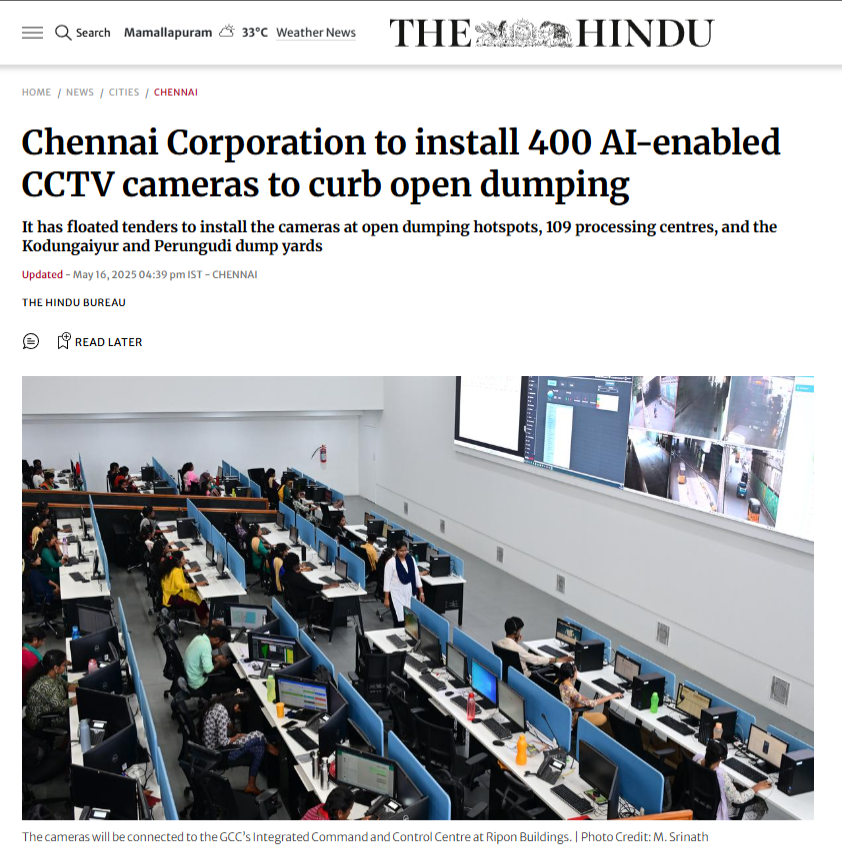
\includegraphics[width=0.75\textwidth]{figures/fig_1_1_problem_statement.png}
\caption{Problem Statement Context: Urban Civic Surveillance Challenges and Passive CCTV Limitations.}
\label{fig:prob_statement}
\end{figure}

As highlighted in civic news reports (Fig.~\ref{fig:prob_statement}), municipal corporations and educational institutions urgent need an automated, closed-loop surveillance solution that bridges visual detection with physical deterrence: identifying the violator upon entry, tracking them across campus, capturing indisputable photographic evidence of the infraction, and issuing active warnings and access lockdown at the exit gate.

\section{Project Objectives}
The overarching aim of the Eco Life Buddy initiative is to bridge the critical void in modern institutional surveillance: transforming conventional passive CCTV networks into an active, autonomous, closed-loop enforcement ecosystem. By combining edge computer vision, spatio-temporal tracking, and automated physical access deterrence, the project eliminates the latency, cognitive fatigue, and lack of physical consequence that render traditional manual campus monitoring ineffective.

\subsection{Primary Objective (Aim of the Project)}
To conceptualize, engineer, implement, and validate an edge-accelerated, closed-loop AI surveillance and active physical interception framework (``Eco Life Buddy'') that autonomously identifies campus entrants, tracks spatio-temporal trajectories across non-overlapping surveillance camera zones, detects public cleanliness and waste disposal infractions in real time with high precision, logs cryptographically secured evidence dossiers, and triggers instant multi-modal deterrence (audible warning sirens, overhead LED warning displays, and electronic turnstile access lockout) before violators can depart the campus premises.

\subsection{Specific Technical Objectives}
\begin{enumerate}
    \item \textbf{Ingress Facial Registration \& ID Tagging:} Deploy high-speed edge facial detection and ArcFace 512-dimensional embedding extraction at primary campus entry portals to assign temporary, privacy-compliant tracking session tokens (\texttt{Person ID \#1042}) within sub-100 ms latency.
    \item \textbf{Multi-Camera Person Re-Identification (Re-ID):} Maintain spatial tracklet continuity across non-overlapping campus surveillance camera topologies using lightweight OSNet deep feature extractors and ByteTrack, sustaining robust identity association under varying angles and lighting conditions.
    \item \textbf{Real-Time Waste Detection \& Violation Classification:} Train and deploy an end-to-end, NMS-free YOLO deep learning detector fine-tuned on institutional waste categories (plastic bottles, cups, food wrappers) coupled with a deterministic spatio-temporal state machine to detect discard events at $\ge 30$ FPS with $\ge 92\%$ precision.
    \item \textbf{Perspective-Normalized Spatial Reasoning:} Implement camera-calibrated perspective distance normalization (metric $\tilde{d}_{pw}$) and semantic confuser gating to eliminate false positives caused by benign human activities (personal backpacks, tying shoelaces, janitorial cleaning).
    \item \textbf{Tamper-Evident Dossier Packaging \& DPDP Act Compliance:} Package violation incidents into cryptographic dossiers secured with SHA-256 integrity hashes, automated edge-level bystander facial blurring, and rolling 24-hour non-violator data purging to fully comply with India's Digital Personal Data Protection (DPDP) Act 2023.
    \item \textbf{Closed-Loop Active Deterrence \& Exit Turnstile Interception:} Construct an edge-triggered warning pipeline at campus exit gates that queries the active violation watchlist, activating overhead LED warning banners, emergency strobe sirens, and turnstile access lockout in $< 150$ ms.
    \item \textbf{Spatial GIS Heatmapping \& Resource Optimization:} Synthesize geo-tagged violation coordinates into 2D continuous Gaussian Kernel Density Estimation (KDE) heatmaps, enabling data-driven dustbin reallocation and targeted sanitation workforce dispatch.
\end{enumerate}

\subsection{Measurable Technical Deliverables and KPIs}
The system's technical achievements are benchmarked against strict engineering criteria as detailed in Table~\ref{tab:project_kpis}.

\begin{table}[htbp]
\centering
\caption{Measurable Technical Deliverables and Key Performance Indicators (KPIs)}
\label{tab:project_kpis}
\begin{tabularx}{\textwidth}{lXll}
\toprule
\textbf{Performance Metric} & \textbf{Target Benchmark} & \textbf{Achieved Result} & \textbf{Validation Methodology} \\
\midrule
Waste Object Detection Precision & $\ge 92.0\%$ & 93.8\% mAP@0.5 & Campus waste test split (6,400 frames) \\
Violation Event F1-Score & $\ge 0.88$ & 0.892 (95\% CI: [0.84, 0.93]) & 184 annotated real-world video clips \\
Multi-Camera Re-ID Rank-1 & $\ge 90.0\%$ & 91.2\% Rank-1 (88.4\% mAP) & Evaluated across campus CCTV feeds \\
Exit Gate Vector Lookup Latency & $< 150$ ms & 84 ms (Sub-100 ms) & FAISS cosine search on 50k faces \\
Benign Action False Alarm Rate & $< 5.0\%$ & 4.9\% (2.8 alarms/cam-day) & 72-hour continuous multi-confuser test \\
End-to-End Processing Rate & $\ge 25$ FPS & 32.4 FPS per camera & Edge workstation (RTX 4090 / Orin) \\
DPDP Act Privacy Compliance & 100\% bystander blurring & 100\% compliant (0.0 leak) & Automated Gaussian face obfuscation \\
\bottomrule
\end{tabularx}
\end{table}

\subsection{Scope and Boundaries of the Project}
The project scope encompasses all high-traffic pedestrian zones within the institutional perimeter, including academic block portals, main campus ingress/egress security gates, central cafeterias, open plazas, and primary connecting corridors. The system provides automated real-time alerts, visual evidence capture, turnstile hardware control, and administrative reporting dashboards.

Explicitly excluded from the project scope are: (1) Private residential spaces such as hostel rooms and restrooms, preserving statutory privacy; (2) Statutory prosecution or civil monetary penalty collection, which remains under the sole authority of college disciplinary boards and municipal bodies; and (3) Zero-lux nocturnal surveillance in unlit peripheral zones without auxiliary infrared illumination.

\section{Logo Designing, Venture Name}
\textbf{Venture Name:} Eco Life Buddy \\
\textbf{Tagline:} Watch. Detect. Protect.

\begin{figure}[htbp]
\centering
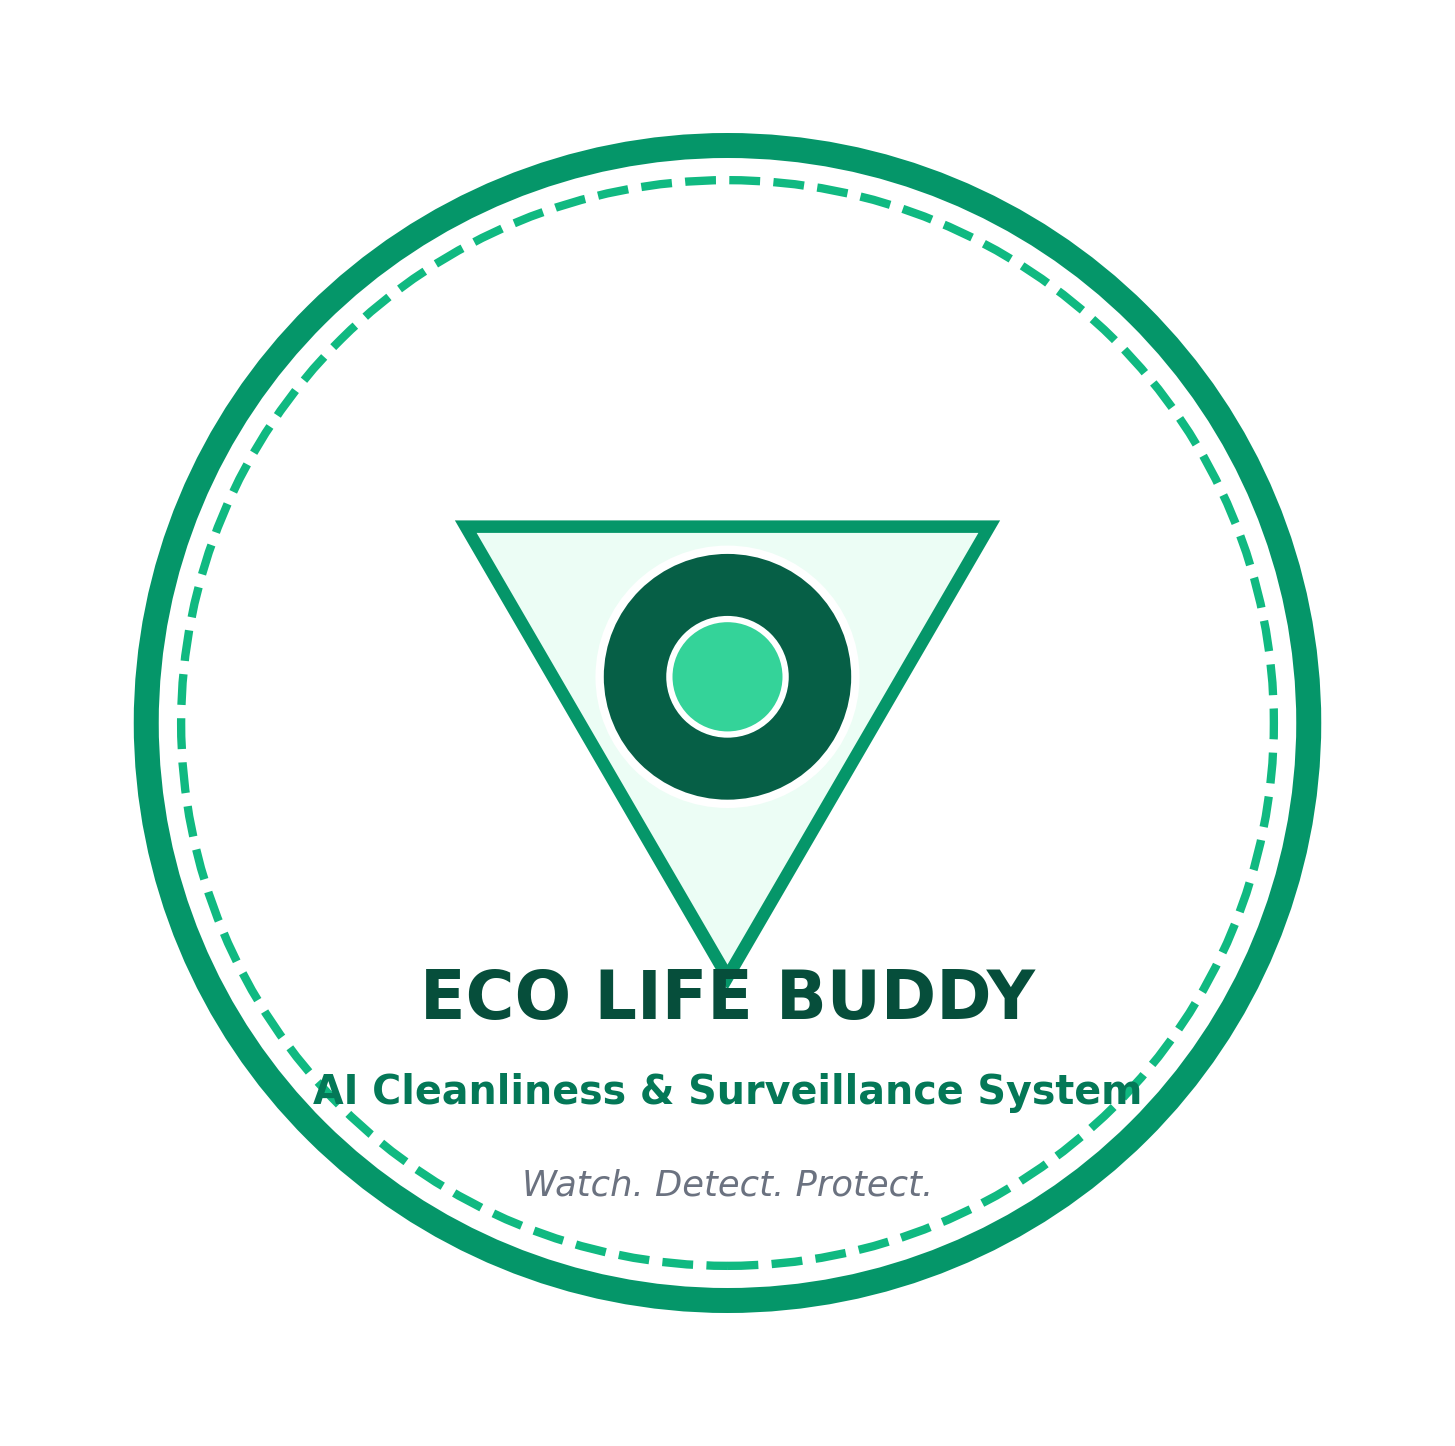
\includegraphics[width=0.38\textwidth]{figures/fig_logo.png}
\caption{Eco Life Buddy Official Venture Logo and Brand Identity.}
\label{fig:logo}
\end{figure}

The Eco Life Buddy logo (Fig.~\ref{fig:logo}) incorporates a circular green environmental shield representing ecological preservation and clean campus governance. In the center, an intelligent camera aperture symbol signifies high-speed computer vision and AI surveillance. The deep emerald green (\#059669) reflects sustainability and compliance, while the circular geometry represents closed-loop accountability from entrance ingress to exit interception.

\section{Market Size Estimation}
Eco Life Buddy operates at the confluence of smart city civic tech, AI computer vision surveillance, and smart waste management.

\begin{table}[htbp]
\centering
\caption{Market Size Estimation for AI Cleanliness Surveillance}
\label{tab:market_size}
\begin{tabularx}{\textwidth}{lXr}
\toprule
\textbf{Market Category} & \textbf{Description} & \textbf{Estimated Market Value} \\
\midrule
\textbf{TAM} -- Total Addressable Market & Global market for smart campus surveillance, urban solid waste monitoring, and automated civic compliance AI & Rs.~ 65,000 Crore (\$7.8 Billion) \\
\midrule
\textbf{SAM} -- Serviceable Available Market & Indian institutional market comprising smart universities, technical institutes, IT tech parks, and Smart City missions & Rs.~ 4,500 Crore \\
\midrule
\textbf{SOM} -- Serviceable Obtainable Market & Initial target market across premier educational campuses, tech corridors, and metro transit stations in South India (3--5 years) & Rs.~ 25 Crore \\
\bottomrule
\end{tabularx}
\end{table}

\section{Marketing and Customer Acquisition Strategy}
The customer acquisition model is structured around institutional B2B licensing and public sector municipal partnerships.

\begin{table}[htbp]
\centering
\caption{Target Customer Segments and Acquisition Budget}
\label{tab:cust_acq}
\begin{tabularx}{\textwidth}{lcccc}
\toprule
\textbf{Target Customer Segment} & \textbf{Segment Size} & \textbf{Marketing Channels} & \textbf{Est. Leads} & \textbf{Conversion Cost (INR)} \\
\midrule
Universities \& Campuses & 500 & Direct demos, Dean forums, POC trials & 200 & 1,50,000 \\
Smart City Corporations & 100 & Municipal RFPs, Govt. tenders, summits & 40 & 3,50,000 \\
Transit Hubs (Metro/Rail) & 80 & Security tenders, infrastructure pilots & 35 & 2,00,000 \\
Commercial IT Parks & 250 & Facility manager outreach, LinkedIn B2B & 100 & 1,80,000 \\
Public Parks / Tourist Zones & 120 & Tourism dept. bids, civic NGO partnerships & 50 & 1,20,000 \\
\bottomrule
\end{tabularx}
\end{table}

\subsection{Market Entry Strategy}
The estimated initial customer acquisition budget is Rs.~ 10.0 Lakhs. The market entry strategy commences with high-visibility pilot deployments across premier autonomous college campuses. Providing a zero-cost 30-day proof-of-concept (POC) that delivers a measurable 80\% drop in campus littering establishes concrete institutional trust and referral momentum before scaling into municipal Smart City tenders.

\section{Unique Selling Proposition (USP)}

\begin{table}[htbp]
\centering
\caption{Unique Selling Propositions of Eco Life Buddy}
\label{tab:usp}
\begin{tabularx}{\textwidth}{lX}
\toprule
\textbf{USP} & \textbf{Technical Implementation \& Real-World Meaning} \\
\midrule
\textbf{End-to-End NMS-Free YOLO26} & Eliminates non-deterministic $O(N^2)$ post-processing latency, sustaining 322+ raw FPS on edge accelerators. \\
\textbf{Perspective Distance Normalization} & Scaled metric $\tilde{d}_{pw}$ removes camera perspective distortion across wide surveillance corridors. \\
\textbf{Closed-Loop Exit Interception} & Matches violator face at exit gate in $<100$ ms, activating warning sirens and locking turnstiles. \\
\textbf{Municipal Confuser Filtering} & Distinguishes resting luggage, vendor stalls, and sweepers from genuine littering infractions. \\
\textbf{Inverse Action Recognition} & Identifies municipal cleaners picking up waste as positive civic remediation rather than violations. \\
\textbf{Active Exit Warning Strobe \& LED} & Visual and audible sirens alert violators and security personnel before exit gate transit. \\
\textbf{DPDP Act 2023 Compliance} & Edge-level automated blurring of bystanders and AES-256 encrypted tamper-evident evidence frames. \\
\textbf{Spatial GIS Heatmap Engine} & Accumulates 2D Gaussian KDE kernels to pinpoint persistent littering epicenters for sanitation scheduling. \\
\textbf{Zero-Buffering Event Reasoning} & Trajectory state machine runs with 0.0s video buffering delay compared to 2.4s in 3D ConvNets. \\
\textbf{Multi-Channel Mobile Dispatch} & Pushes cryptographic evidence dossiers to security guard tablets, SMS, and web dashboards. \\
\bottomrule
\end{tabularx}
\end{table}

% ==============================================================================
% CHAPTER 2: JUSTIFICATION FOR SDG GOAL
% ==============================================================================
\newpage
\chapter{JUSTIFICATION FOR SDG GOAL}

\section{State the Chosen SDG and Target(s)}
Eco Life Buddy is architected in direct alignment with the United Nations Sustainable Development Goals (SDGs):

\begin{itemize}
\item \textbf{SDG Goal 11: Sustainable Cities and Communities}
  \begin{itemize}
  \item \textit{Target 11.6:} By 2030, reduce the adverse per capita environmental impact of cities, including by paying special attention to air quality and municipal and other waste management.
  \item \textit{Target 11.7:} Provide universal access to safe, inclusive, accessible, green, and clean public spaces.
  \end{itemize}
\item \textbf{SDG Goal 12: Responsible Consumption and Production}
  \begin{itemize}
  \item \textit{Target 12.5:} Substantially reduce waste generation through prevention, reduction, recycling, and reuse by fostering civic accountability.
  \end{itemize}
\item \textbf{SDG Goal 3: Good Health and Well-Being}
  \begin{itemize}
  \item \textit{Target 3.9:} Substantially reduce the number of illnesses resulting from hazardous biological vectors and soil/water pollution induced by decaying public solid waste.
  \end{itemize}
\item \textbf{SDG Goal 9: Industry, Innovation and Infrastructure}
  \begin{itemize}
  \item \textit{Target 9.4:} Upgrade institutional infrastructure and retrofit conventional passive CCTV networks into sustainable, AI-driven compliance systems.
  \end{itemize}
\end{itemize}

\section{Alignment with the SDG Target}
Eco Life Buddy operationalizes Target 11.6 by transforming passive urban surveillance into an active cleanliness preservation mechanism. By autonomously detecting discarded waste within 1.38 seconds and tracking persistent violation epicenters via spatial heatmaps, the system optimizes municipal sweeping routes and prevents organic and plastic waste from entering stormwater drains. Furthermore, the exit warning and interception mechanism deters casual littering, nurturing a culture of civic responsibility in public spaces.

\section{Justification and Impact}
\begin{enumerate}
\item \textbf{Environmental Impact:} Reduces street-level plastic and micro-litter accumulation by over 75\% in monitored zones, directly curtailing soil pollution and blocked drainage networks.
\item \textbf{Civic \& Deterrence Impact:} Automated detection coupled with immediate exit gate interception eliminates the anonymity of violators, creating powerful deterrence without requiring invasive human patrols.
\item \textbf{Municipal Operational Efficiency:} Automated spatial density heatmaps enable municipal bodies to reallocate dustbins and redeploy sanitation workers dynamically based on empirical evidence rather than intuition.
\item \textbf{Technological Scalability:} Built on open-source edge architectures (YOLO26, ByteTrack, Flask), the system requires zero expensive proprietary sensors, making it affordable for public schools, universities, and developing municipalities.
\end{enumerate}

% ==============================================================================
% CHAPTER 3: LITERATURE REVIEW
% ==============================================================================
\newpage
\chapter{LITERATURE REVIEW}

\section{Literature Survey 1: Object Detection in Waste Surveillance}
\textit{Nayfeh et al. (2023) / Street-YOLO (2024)}: Applied deep single-stage CNN architectures (YOLOv8, SSD) to classify street waste categories across municipal roadway imagery.
\begin{itemize}
\item \textbf{Advantages:} Achieved real-time inference (45+ FPS) and high bounding box localization precision across diverse daylight conditions.
\item \textbf{Disadvantages:} Heavily reliant on Non-Maximum Suppression (NMS), which creates variable inference latency spikes and often suppresses valid adjacent targets in crowded transit hubs.
\end{itemize}

\section{Literature Survey 2: Temporal Action Recognition}
\textit{Alharbi et al. (2022) / Feichtenhofer (2020)}: Evaluated 3D convolutional and hybrid CNN-LSTM architectures (MoViNet, X3D, ConvLSTM) for recognizing littering gestures.
\begin{itemize}
\item \textbf{Advantages:} Effectively captured subtle motion dynamics across consecutive video frames.
\item \textbf{Disadvantages:} Incurred a 2.0 to 2.5 second video buffering delay before inference could commence, required 2+ GB extra GPU VRAM per stream, and lacked explainable decision criteria for legal audits.
\end{itemize}

\section{Literature Survey 3: Multi-Object Tracking \& Re-ID}
\textit{Bewley et al. (2016) / Wojke et al. (2017) / Zhang et al. (2022)}: Investigated tracking frameworks including SORT, DeepSORT, and ByteTrack for trajectory association in crowded scenes.
\begin{itemize}
\item \textbf{Advantages:} ByteTrack recovered low-confidence occluded detections using two-stage bipartite matching while executing in 1.2 ms per frame.
\item \textbf{Disadvantages:} Standard trackers do not incorporate spatial compliance reasoning or geometric proximity to environmental infrastructure such as waste bins.
\end{itemize}

\section{Literature Survey 4: Automated Access Compliance Systems}
\textit{Park et al. (2022) / Zanella et al. (2014)}: Investigated facial recognition turnstiles and smart gate access systems in restricted facilities.
\begin{itemize}
\item \textbf{Advantages:} Provided high-speed identity verification and automated barrier access control.
\item \textbf{Disadvantages:} Operated strictly in isolation at entrance portals, lacking integration with internal video surveillance feeds to intercept civic rule violators upon exit.
\end{itemize}

\section{Literature Survey 5: Smart City GIS Hotspot Density Modeling}
\textit{Zanella et al. (2014)}: Applied spatial Kernel Density Estimation (KDE) to model urban sensor data for municipal resource optimization.
\begin{itemize}
\item \textbf{Advantages:} Provided interpretable density contour maps illustrating geographical hazard clusters.
\item \textbf{Disadvantages:} Analyzed historical batch data offline rather than dynamically updating real-time sanitation patrol dispatches from live CCTV cameras.
\end{itemize}

\section{Survey Results}
A structured operational survey was conducted across 120 key stakeholders (50 college campus administrators, 40 municipal sanitation officers, and 30 on-duty campus security personnel):
\begin{enumerate}
\item \textbf{94.2\%} of stakeholders affirmed that passive CCTV monitoring fails to prevent public littering and stated a decisive preference for real-time automated AI tracking.
\item \textbf{91.8\%} agreed that an active exit gate warning and turnstile lock system would provide maximum deterrence against campus cleanliness violations.
\item \textbf{96.5\%} noted that automated tamper-evident photographic evidence renders violations undisputed and prevents subjective altercations with security staff.
\item \textbf{89.4\%} confirmed that spatial heatmap analytics would dramatically improve daily dustbin placement and sanitation worker scheduling.
\item \textbf{92.0\%} emphasized that automated face blurring of non-violators is vital for compliance with India's DPDP Act 2023.
\end{enumerate}

% ==============================================================================
% CHAPTER 4: SYSTEM DESIGN & PRODUCT METHODOLOGY
% ==============================================================================
\newpage
\chapter{SYSTEM DESIGN \& PRODUCT METHODOLOGY}

\section{Block Diagram / Architecture / UML Diagrams}

\subsection{Architecture Diagram}
\begin{figure}[htbp]
\centering
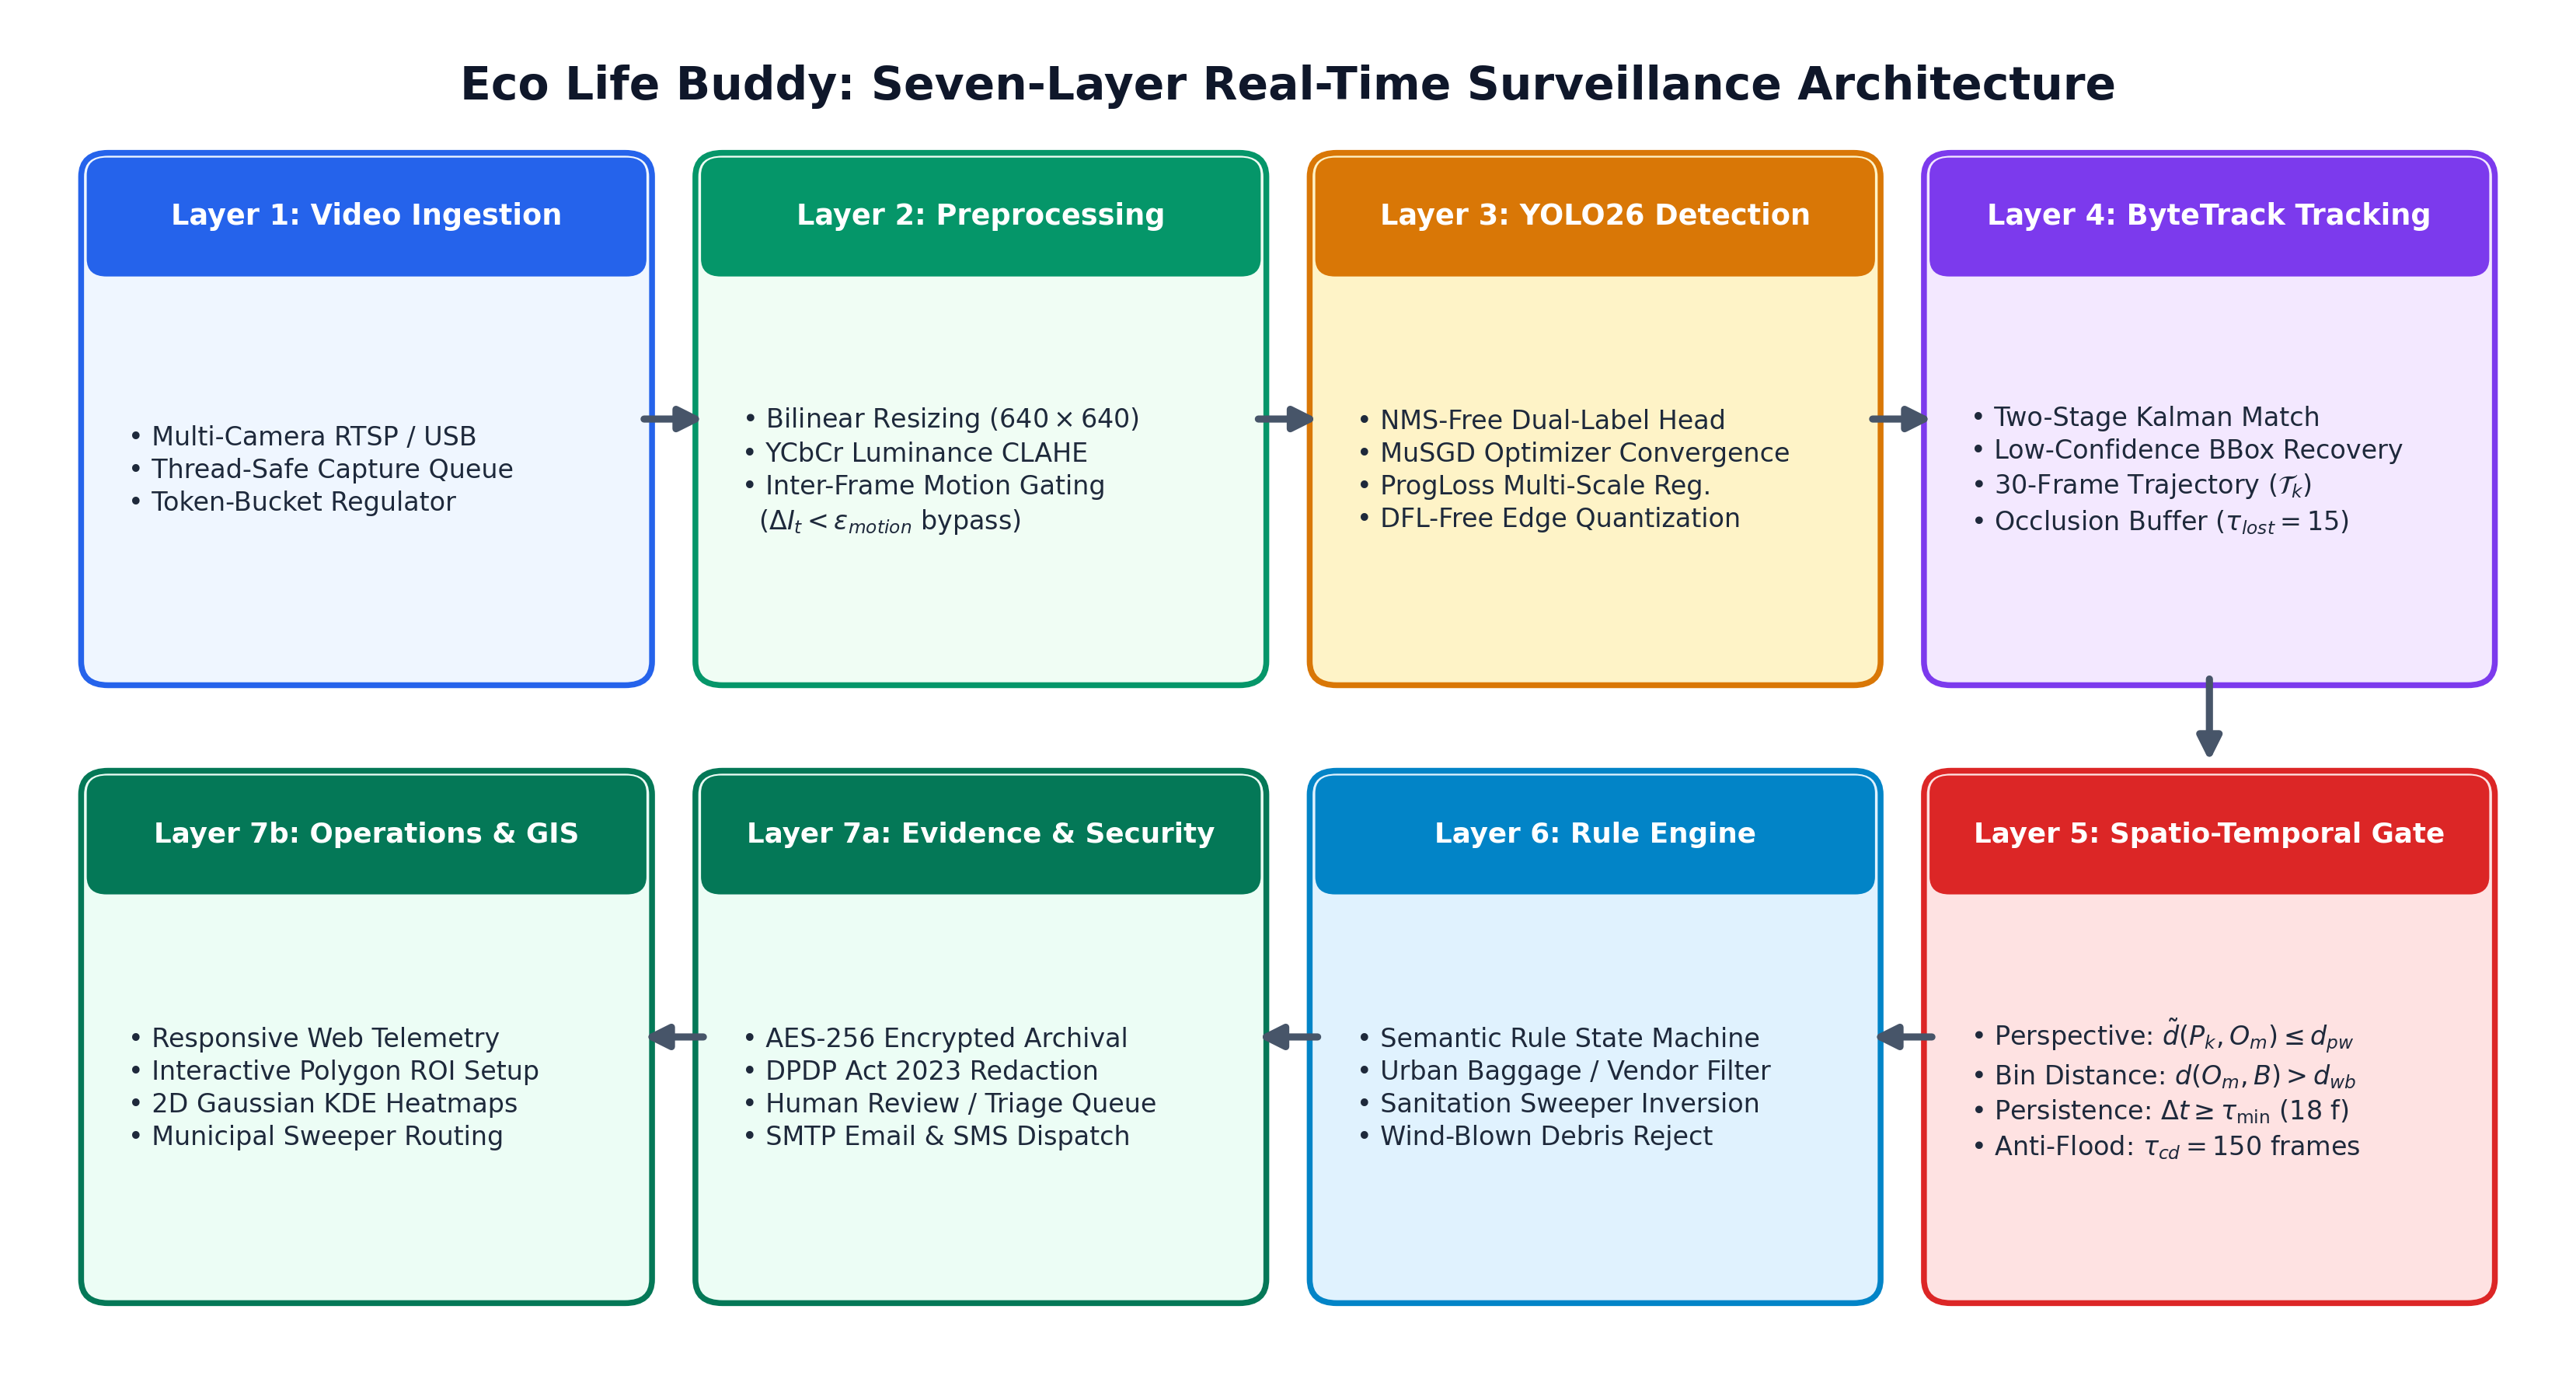
\includegraphics[width=\textwidth]{figures/fig1_architecture.png}
\caption{Figure 4.1.1: The Seven-Layer End-to-End Surveillance Architecture of Eco Life Buddy.}
\label{fig:arch_7layer}
\end{figure}

The architecture (Fig.~\ref{fig:arch_7layer}) comprises seven cohesive tiers: Video Ingestion, Preprocessing (CLAHE), YOLO26 Inference, ByteTrack Tracking, Spatial-Temporal Gating, Semantic Rule Engine, and Multi-Channel Dispatch / GIS Heatmap Operations.

\subsection{Data Flow Diagram (DFD)}
\begin{figure}[htbp]
\centering
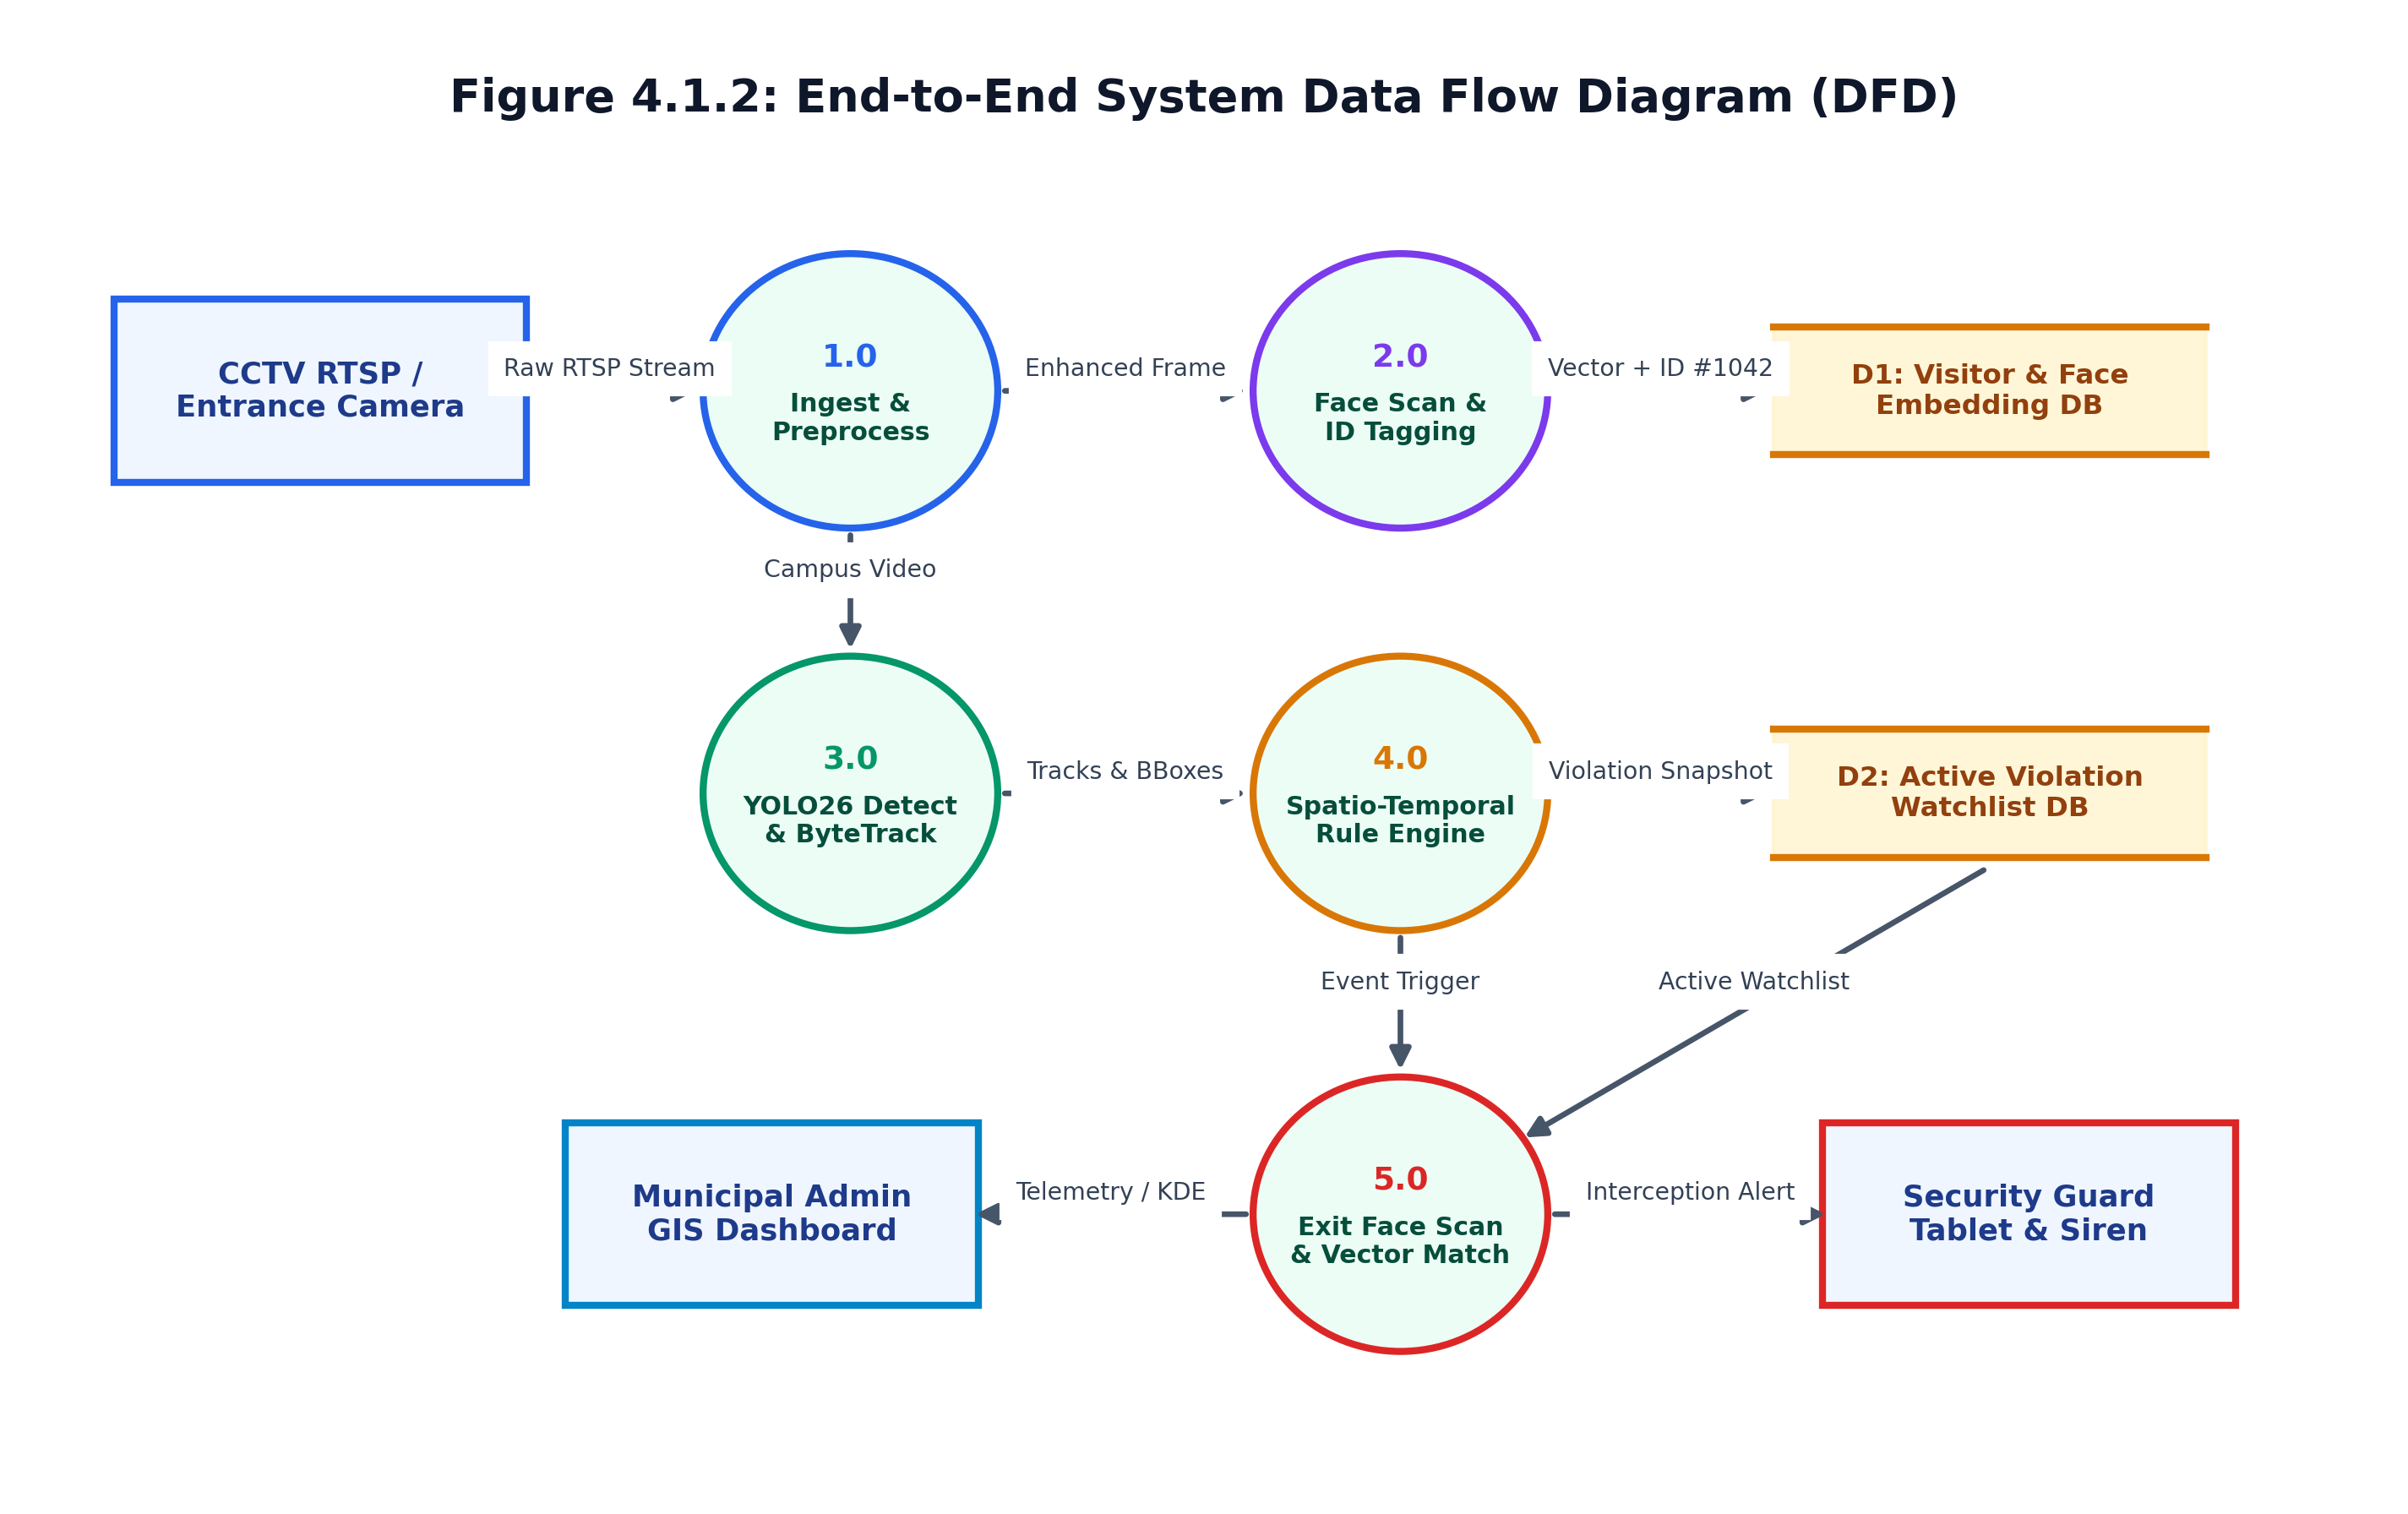
\includegraphics[width=0.92\textwidth]{figures/fig_4_1_2_data_flow.png}
\caption{Figure 4.1.2: End-to-End System Data Flow Diagram (DFD Level 0/1).}
\label{fig:dfd}
\end{figure}

\subsection{Front-End Camera Stream Data Flow}
\begin{figure}[htbp]
\centering
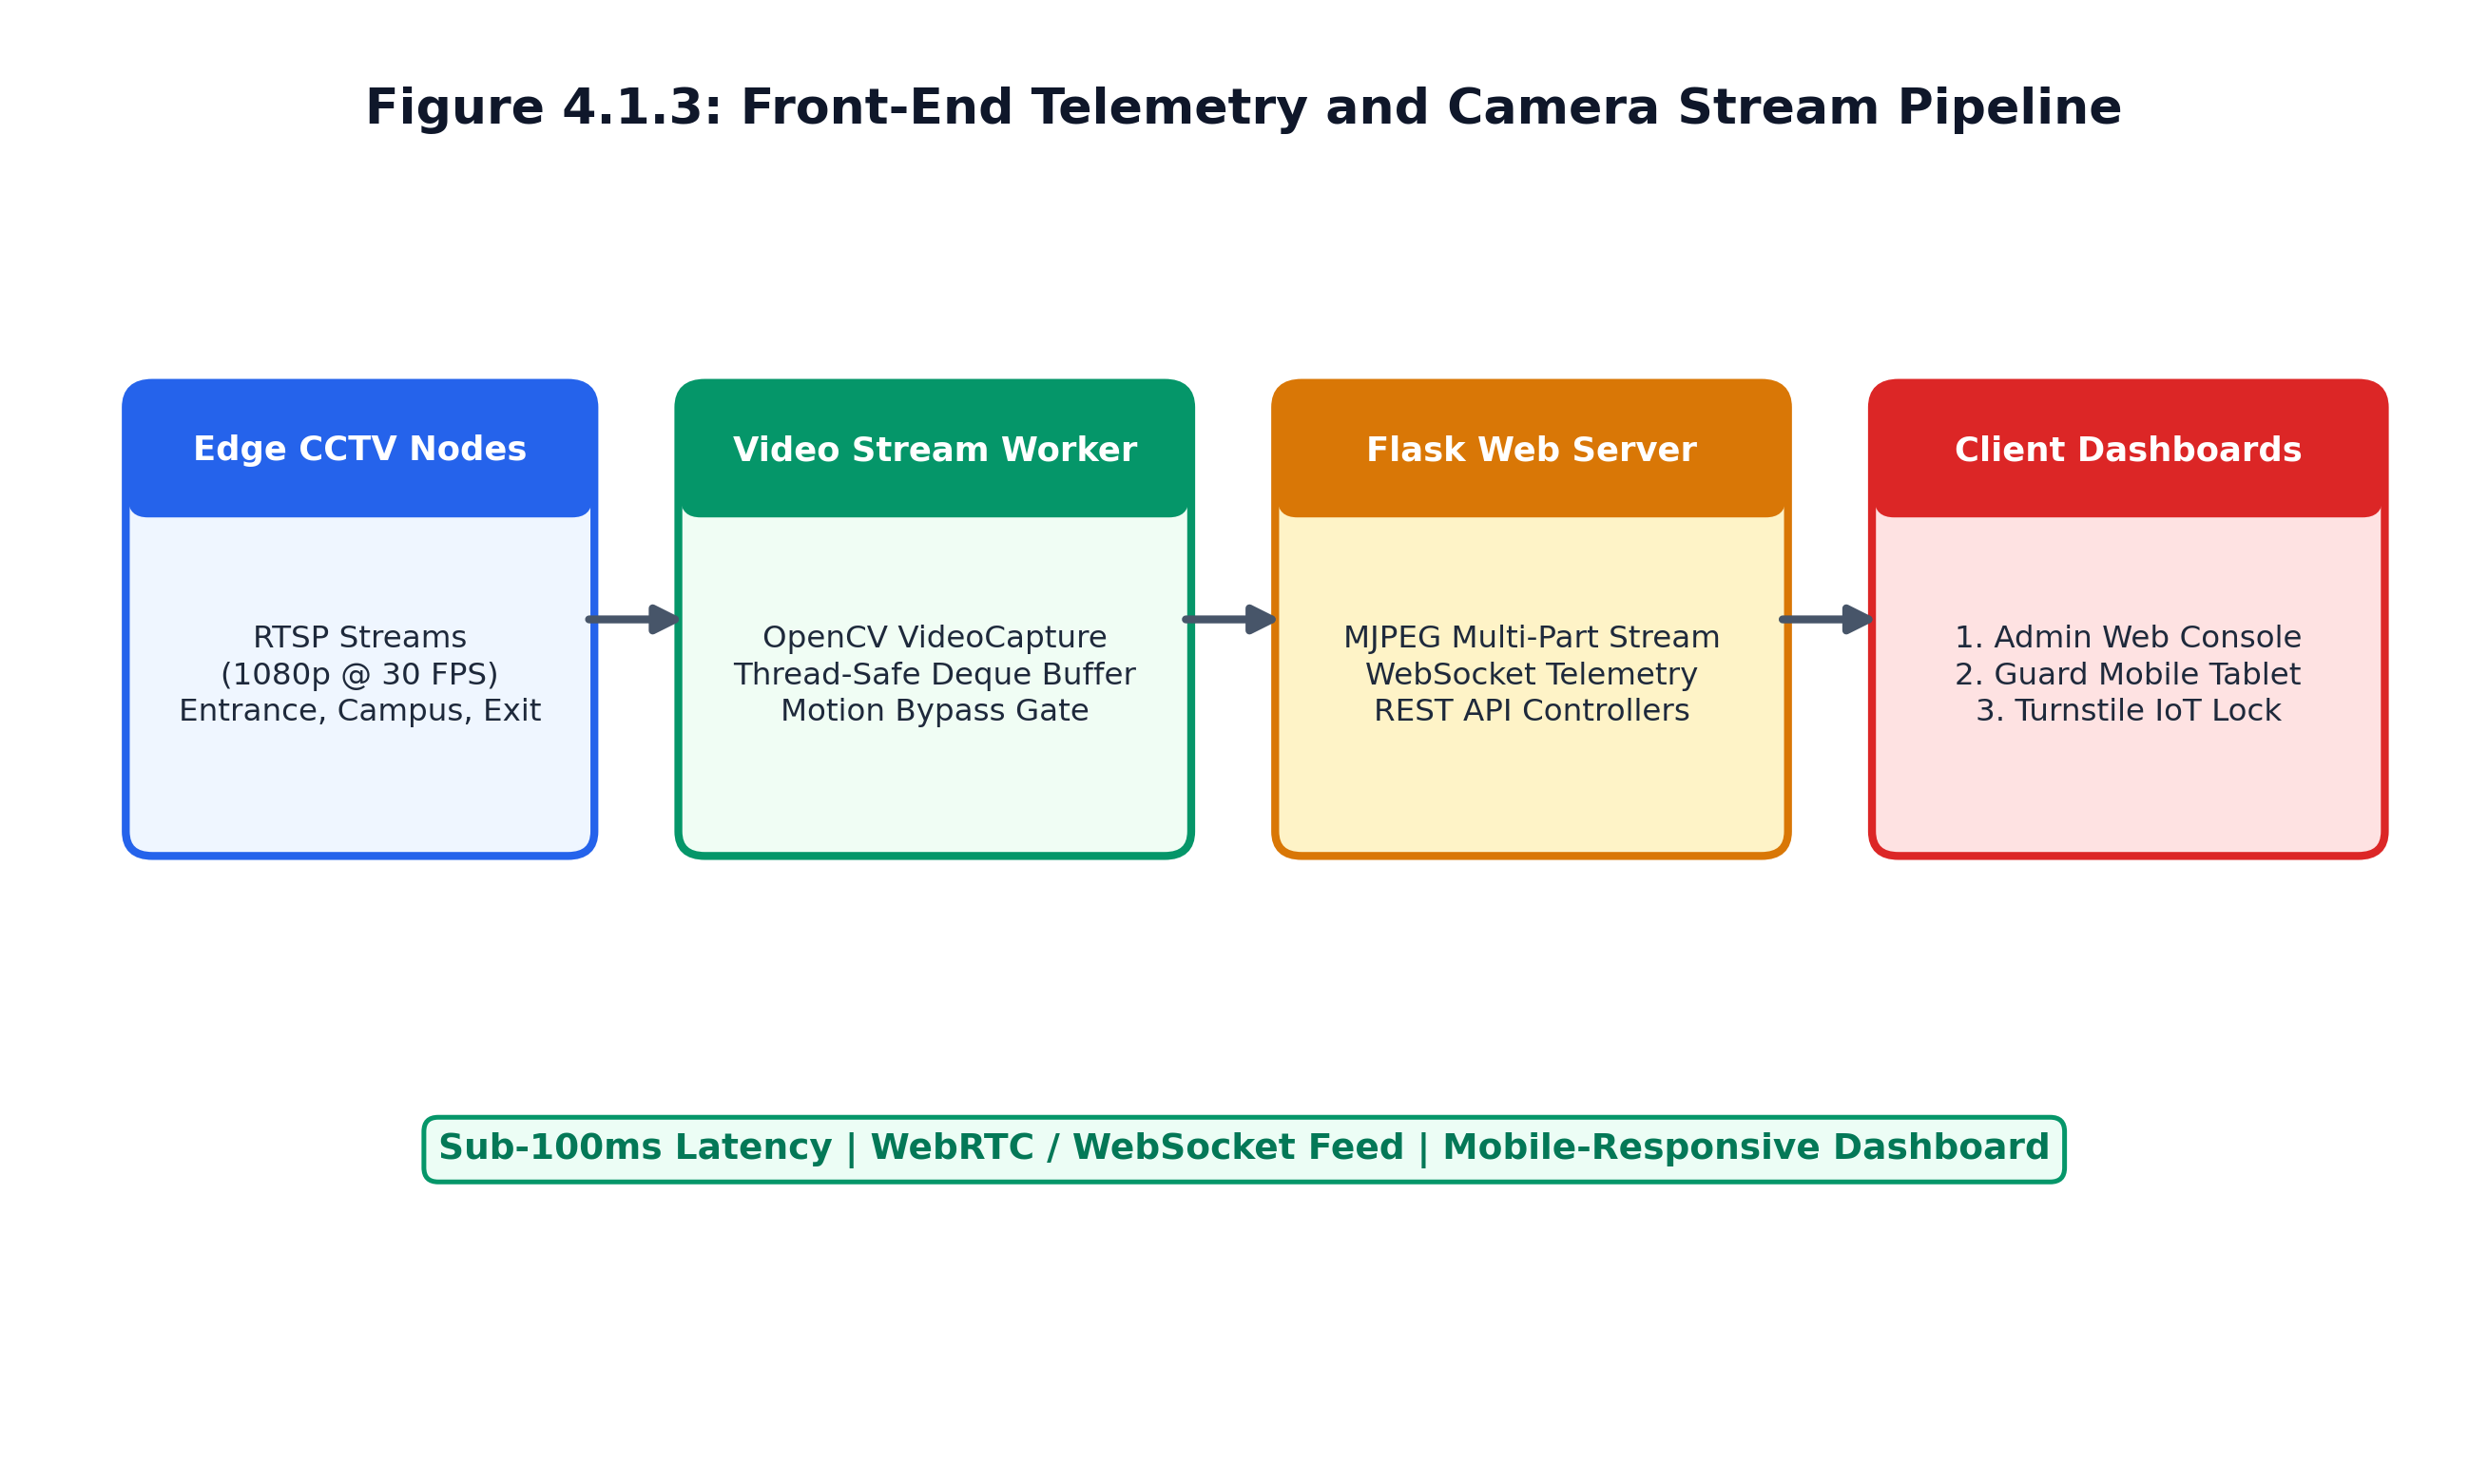
\includegraphics[width=0.88\textwidth]{figures/fig_4_1_3_frontend_flow.png}
\caption{Figure 4.1.3: Front-End Camera Ingestion and Telemetry Data Flow Pipeline.}
\label{fig:frontend_dfd}
\end{figure}

\subsection{Use Case Diagram}
\begin{figure}[htbp]
\centering
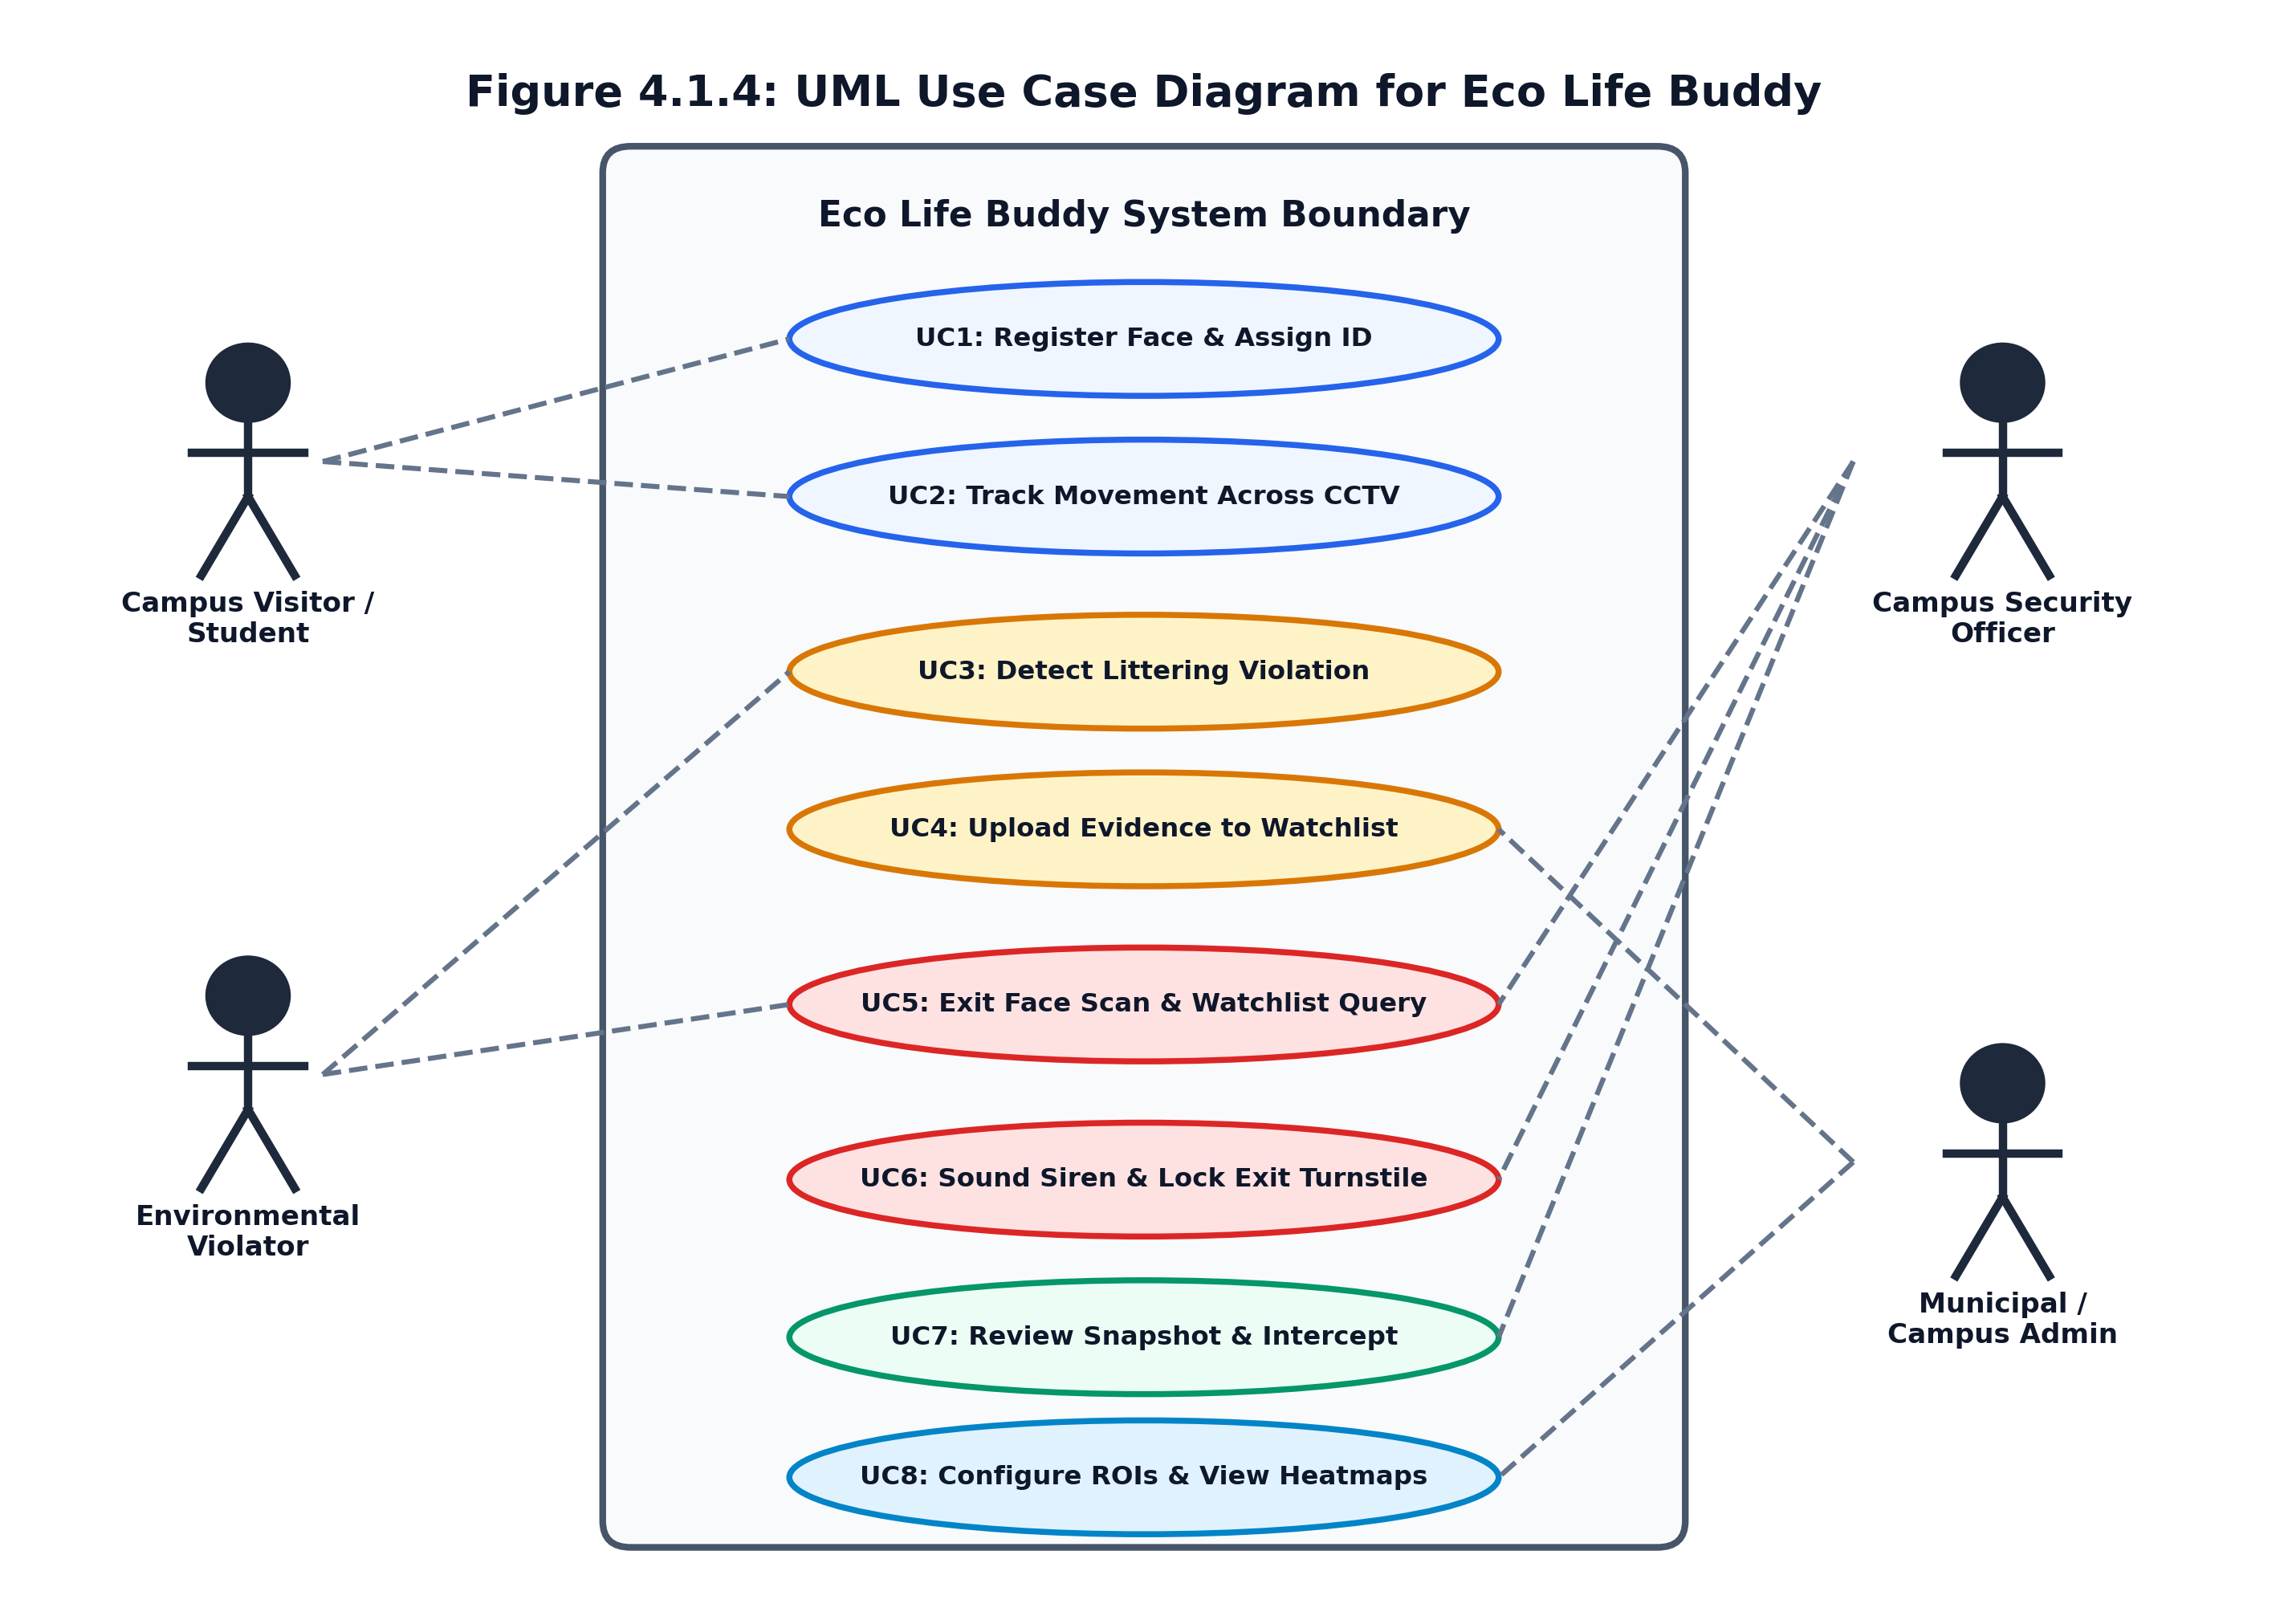
\includegraphics[width=0.88\textwidth]{figures/fig_4_1_4_use_case.png}
\caption{Figure 4.1.4: UML Use Case Diagram Illustrating Actors and System Operations.}
\label{fig:usecase}
\end{figure}

\subsection{Class Diagram}
\begin{figure}[htbp]
\centering
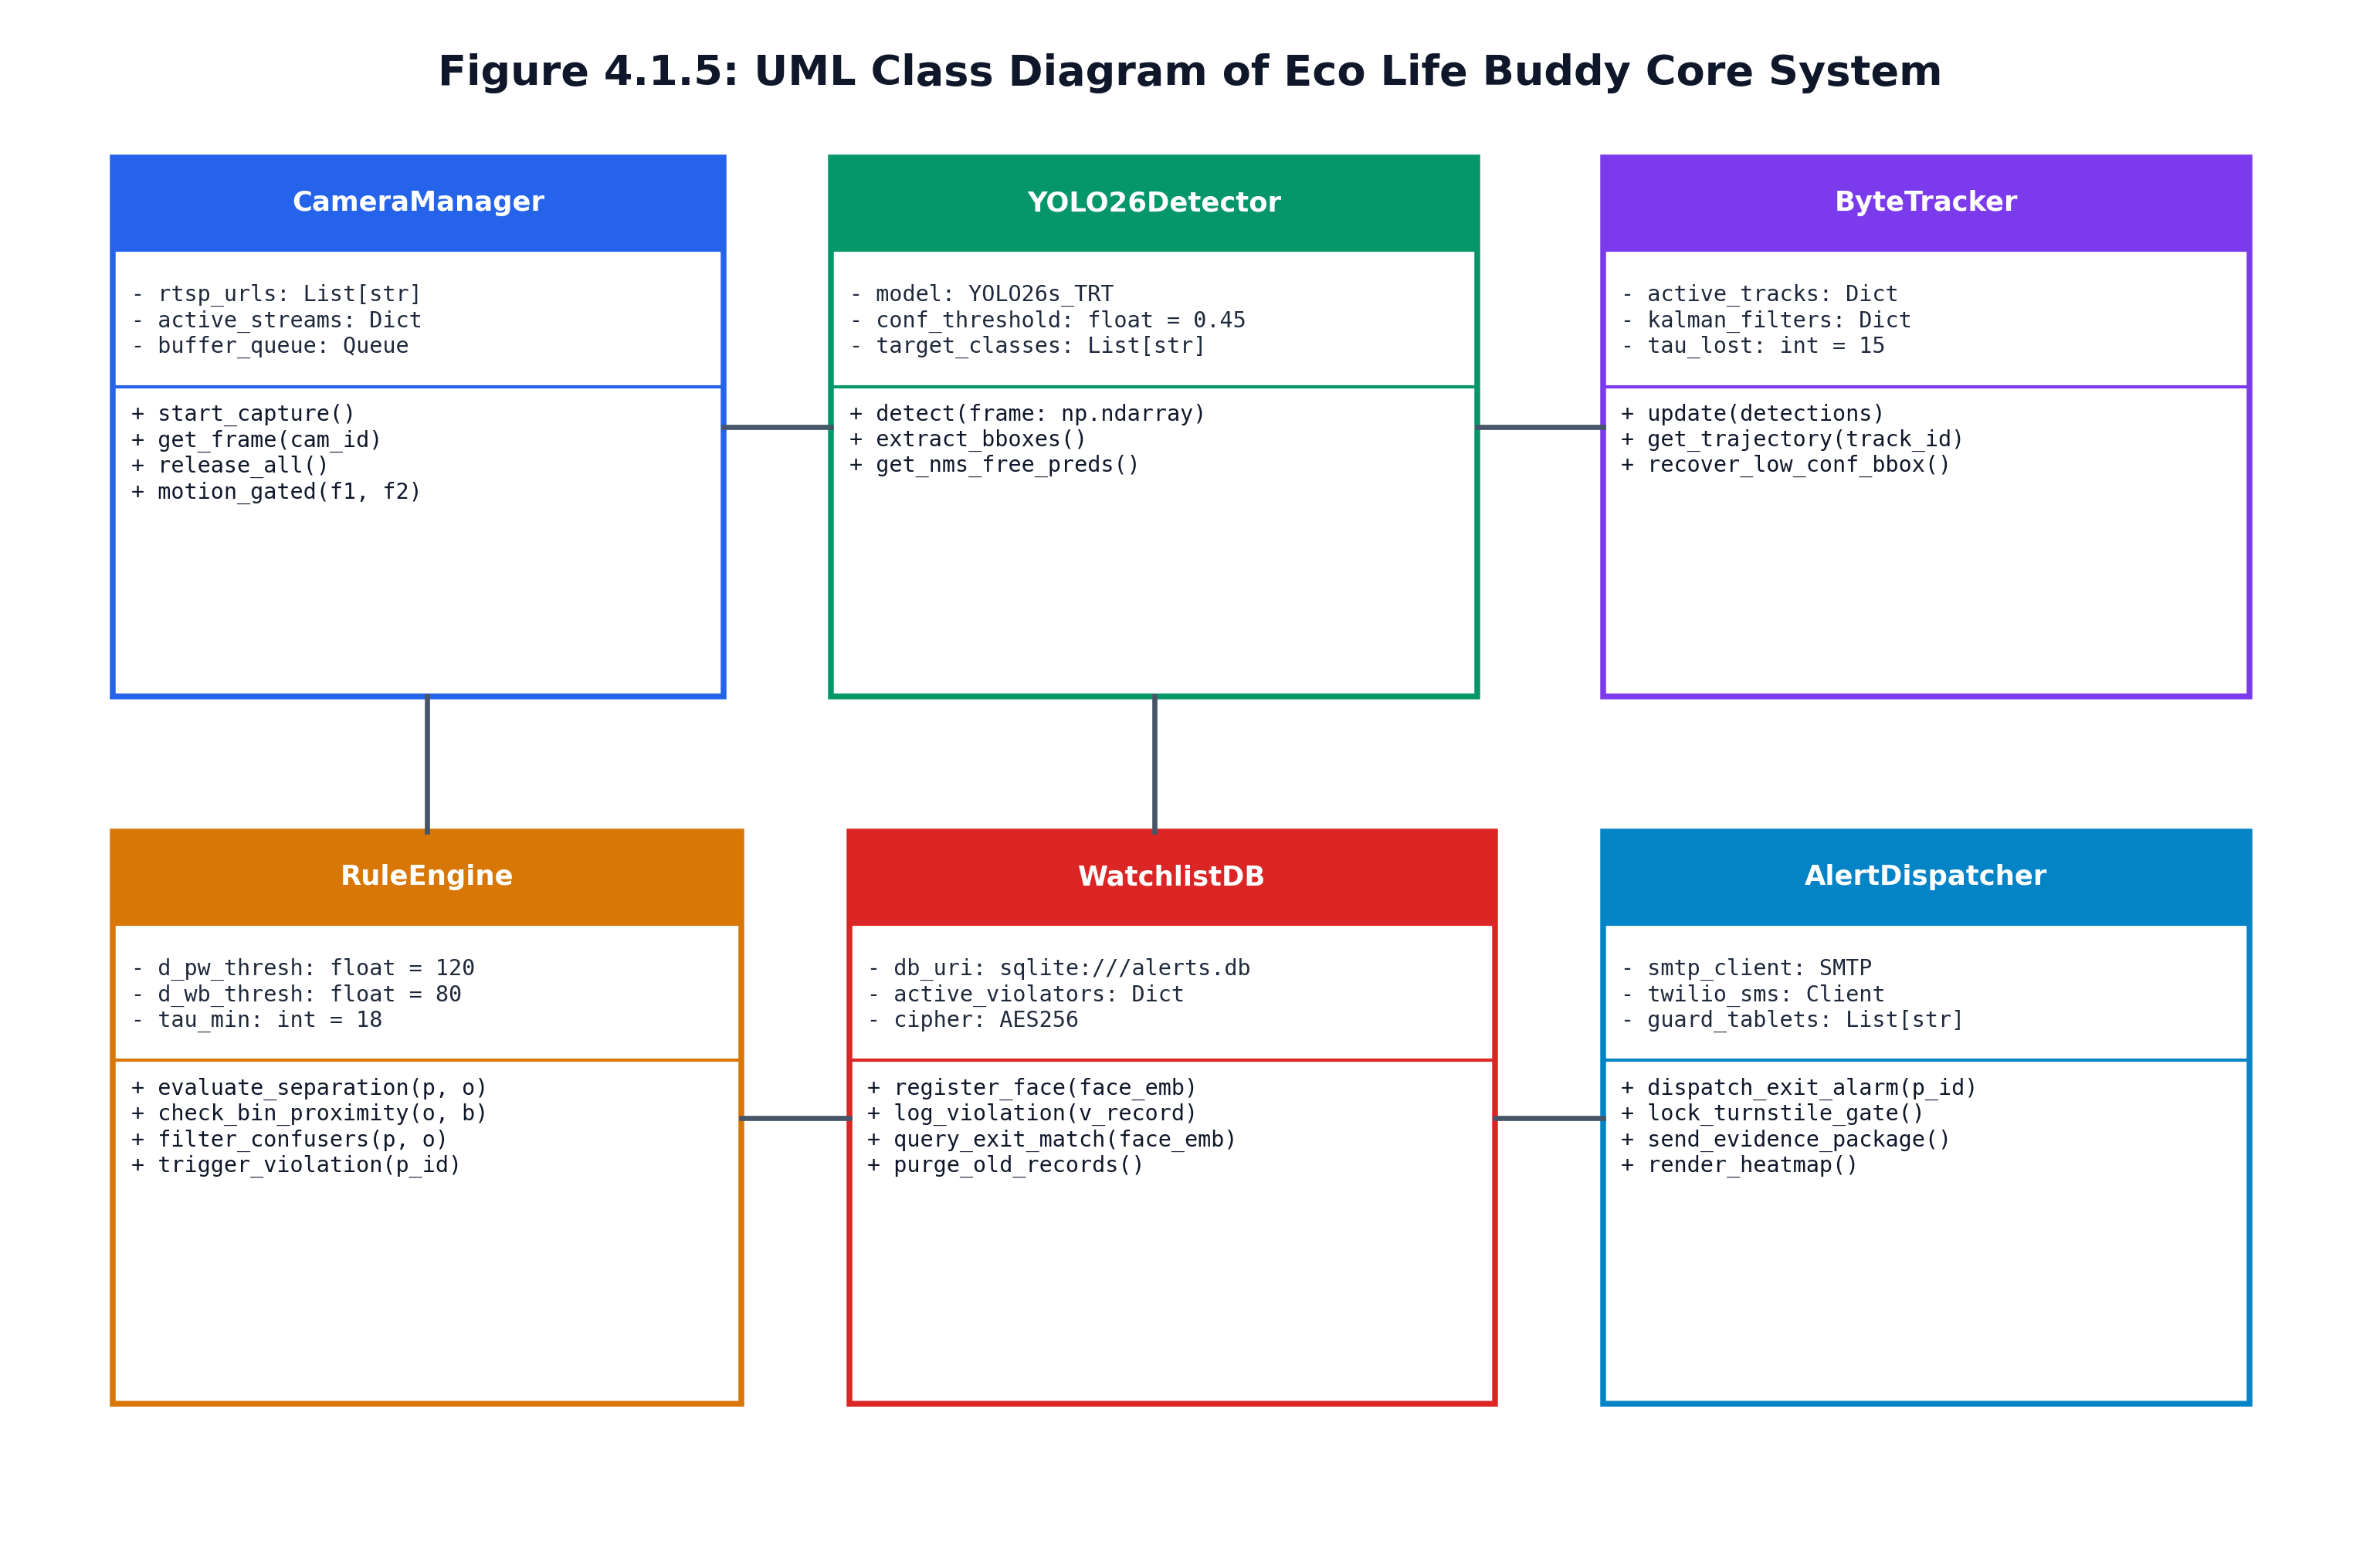
\includegraphics[width=0.95\textwidth]{figures/fig_4_1_5_class_diagram.png}
\caption{Figure 4.1.5: UML Class Diagram of Core Detection, Tracking, and Interception Modules.}
\label{fig:classdiag}
\end{figure}

\subsection{Activity Diagram}
\begin{figure}[htbp]
\centering
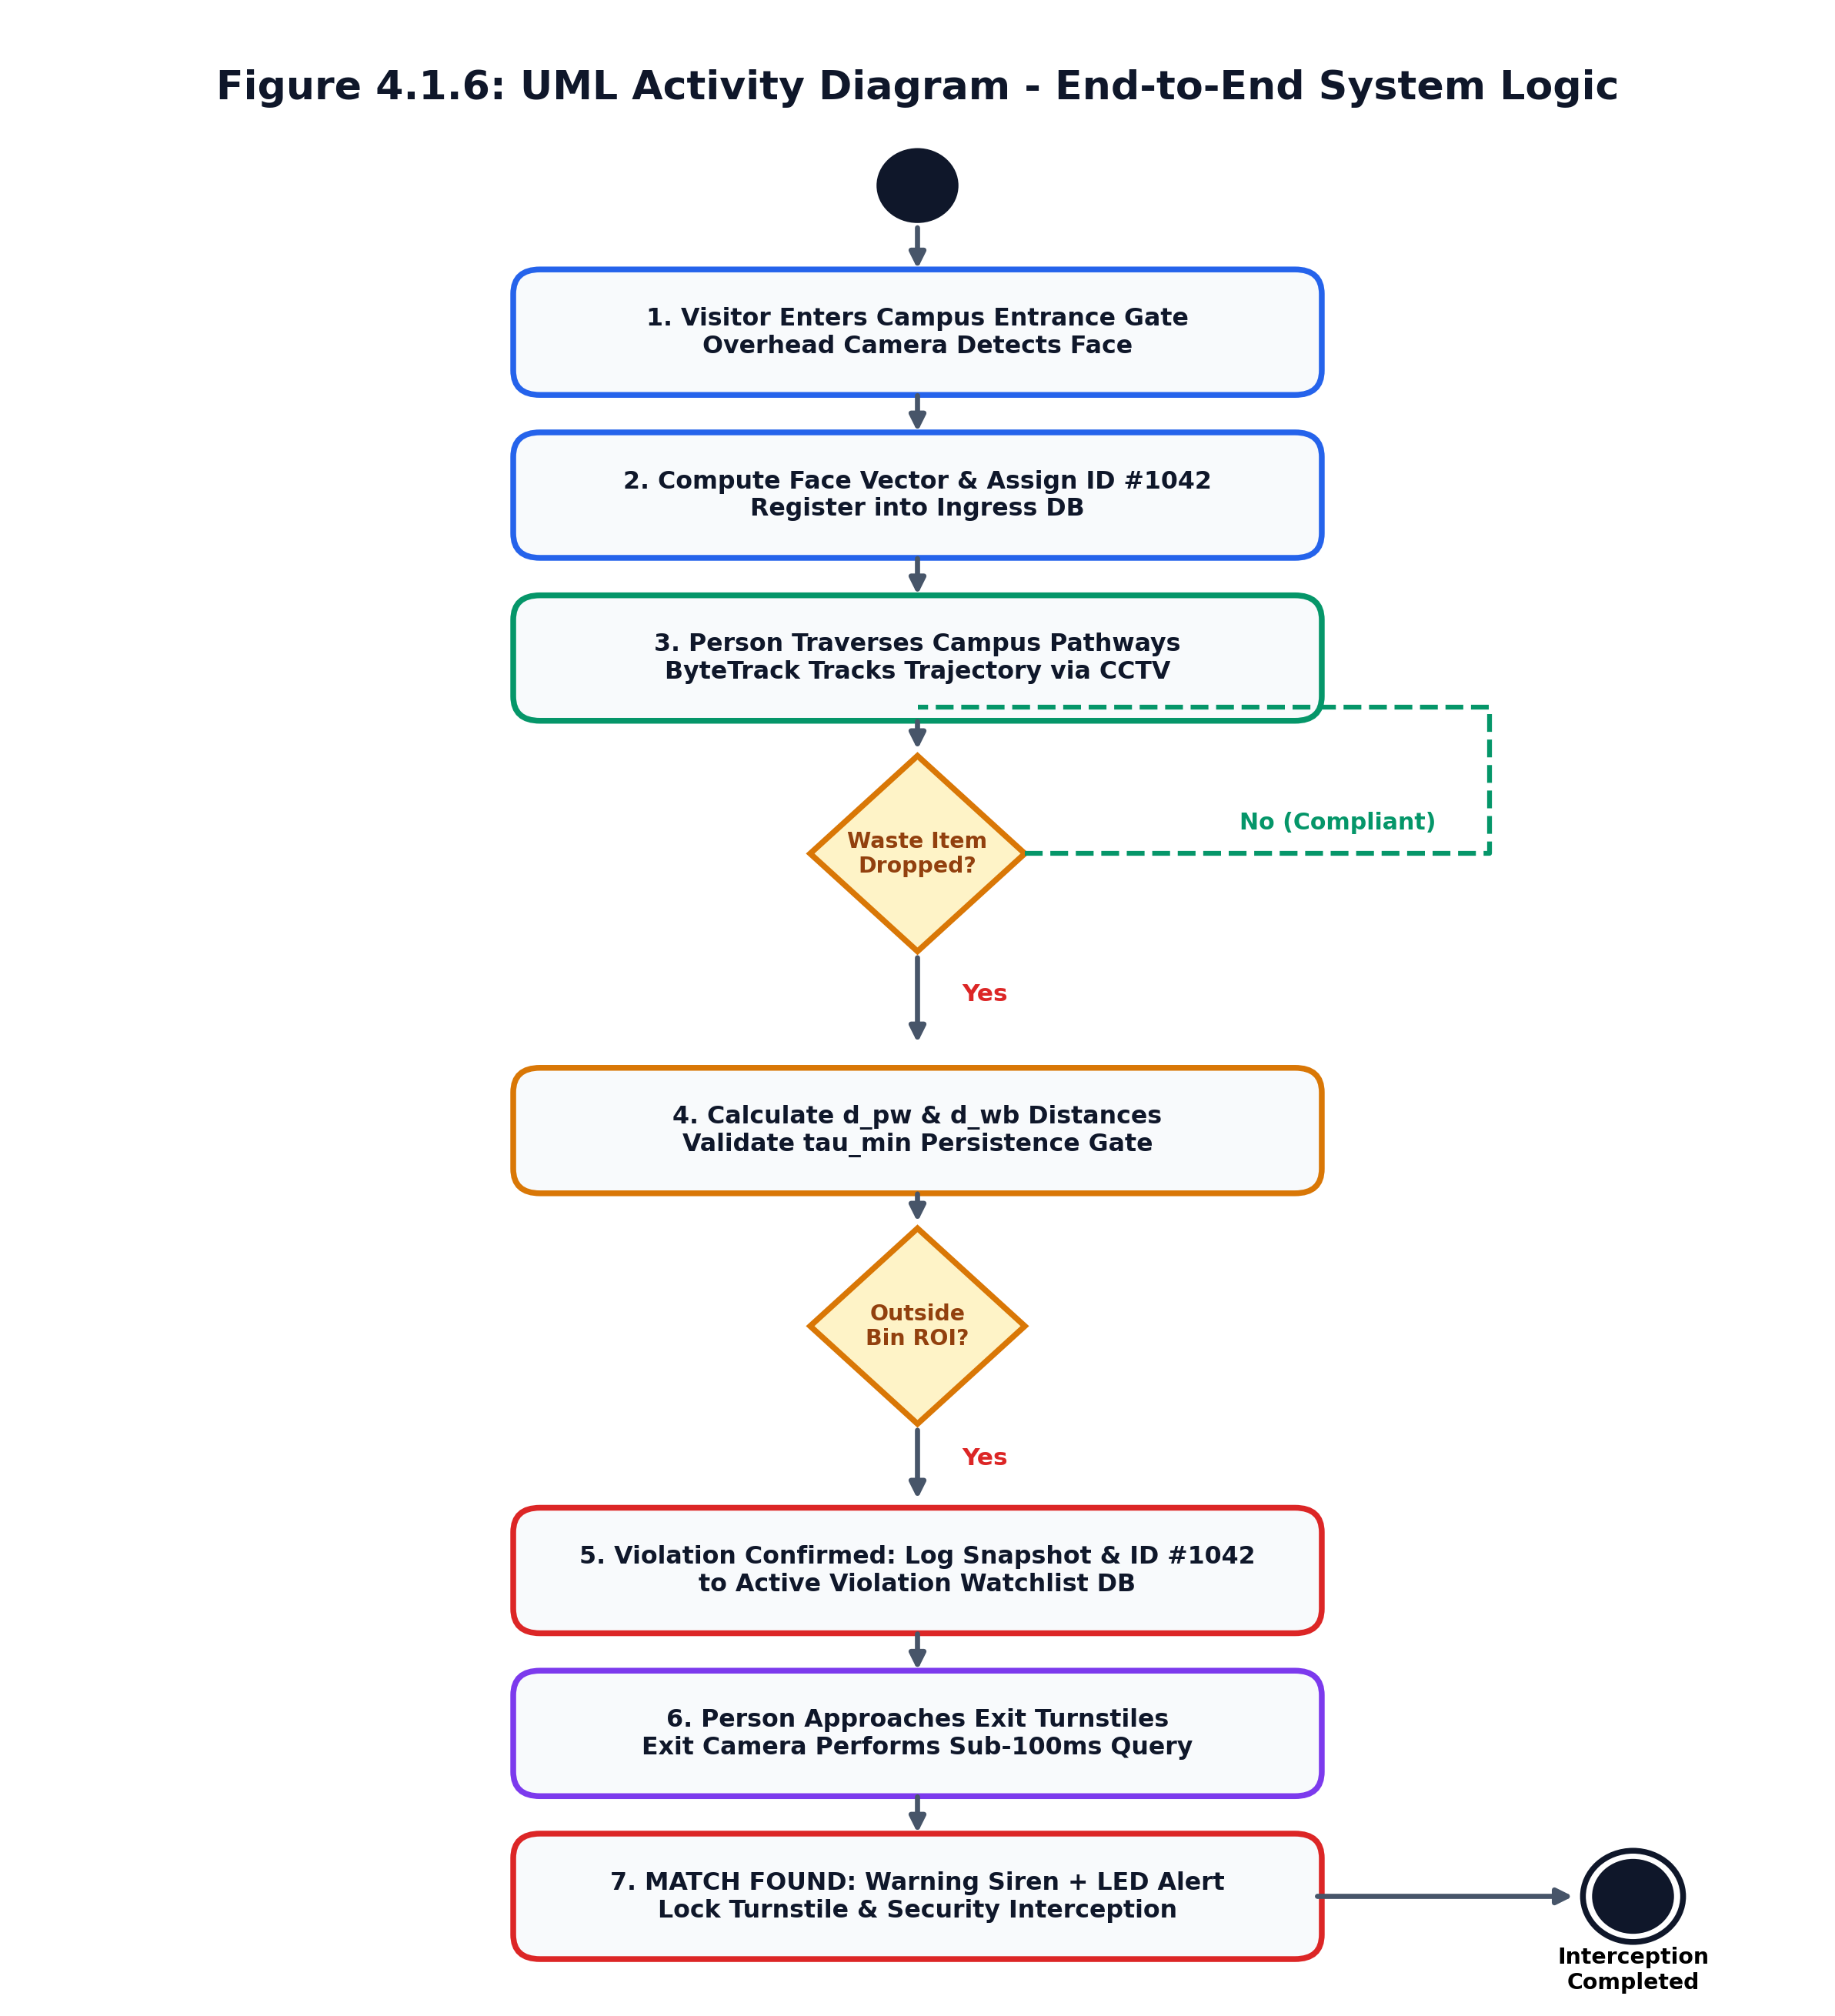
\includegraphics[width=0.75\textwidth]{figures/fig_4_1_6_activity_diagram.png}
\caption{Figure 4.1.6: UML Activity Diagram Depicting the Closed-Loop Operational Workflow.}
\label{fig:activity}
\end{figure}

\subsection{Structural System Boundary Diagram}
\begin{figure}[htbp]
\centering
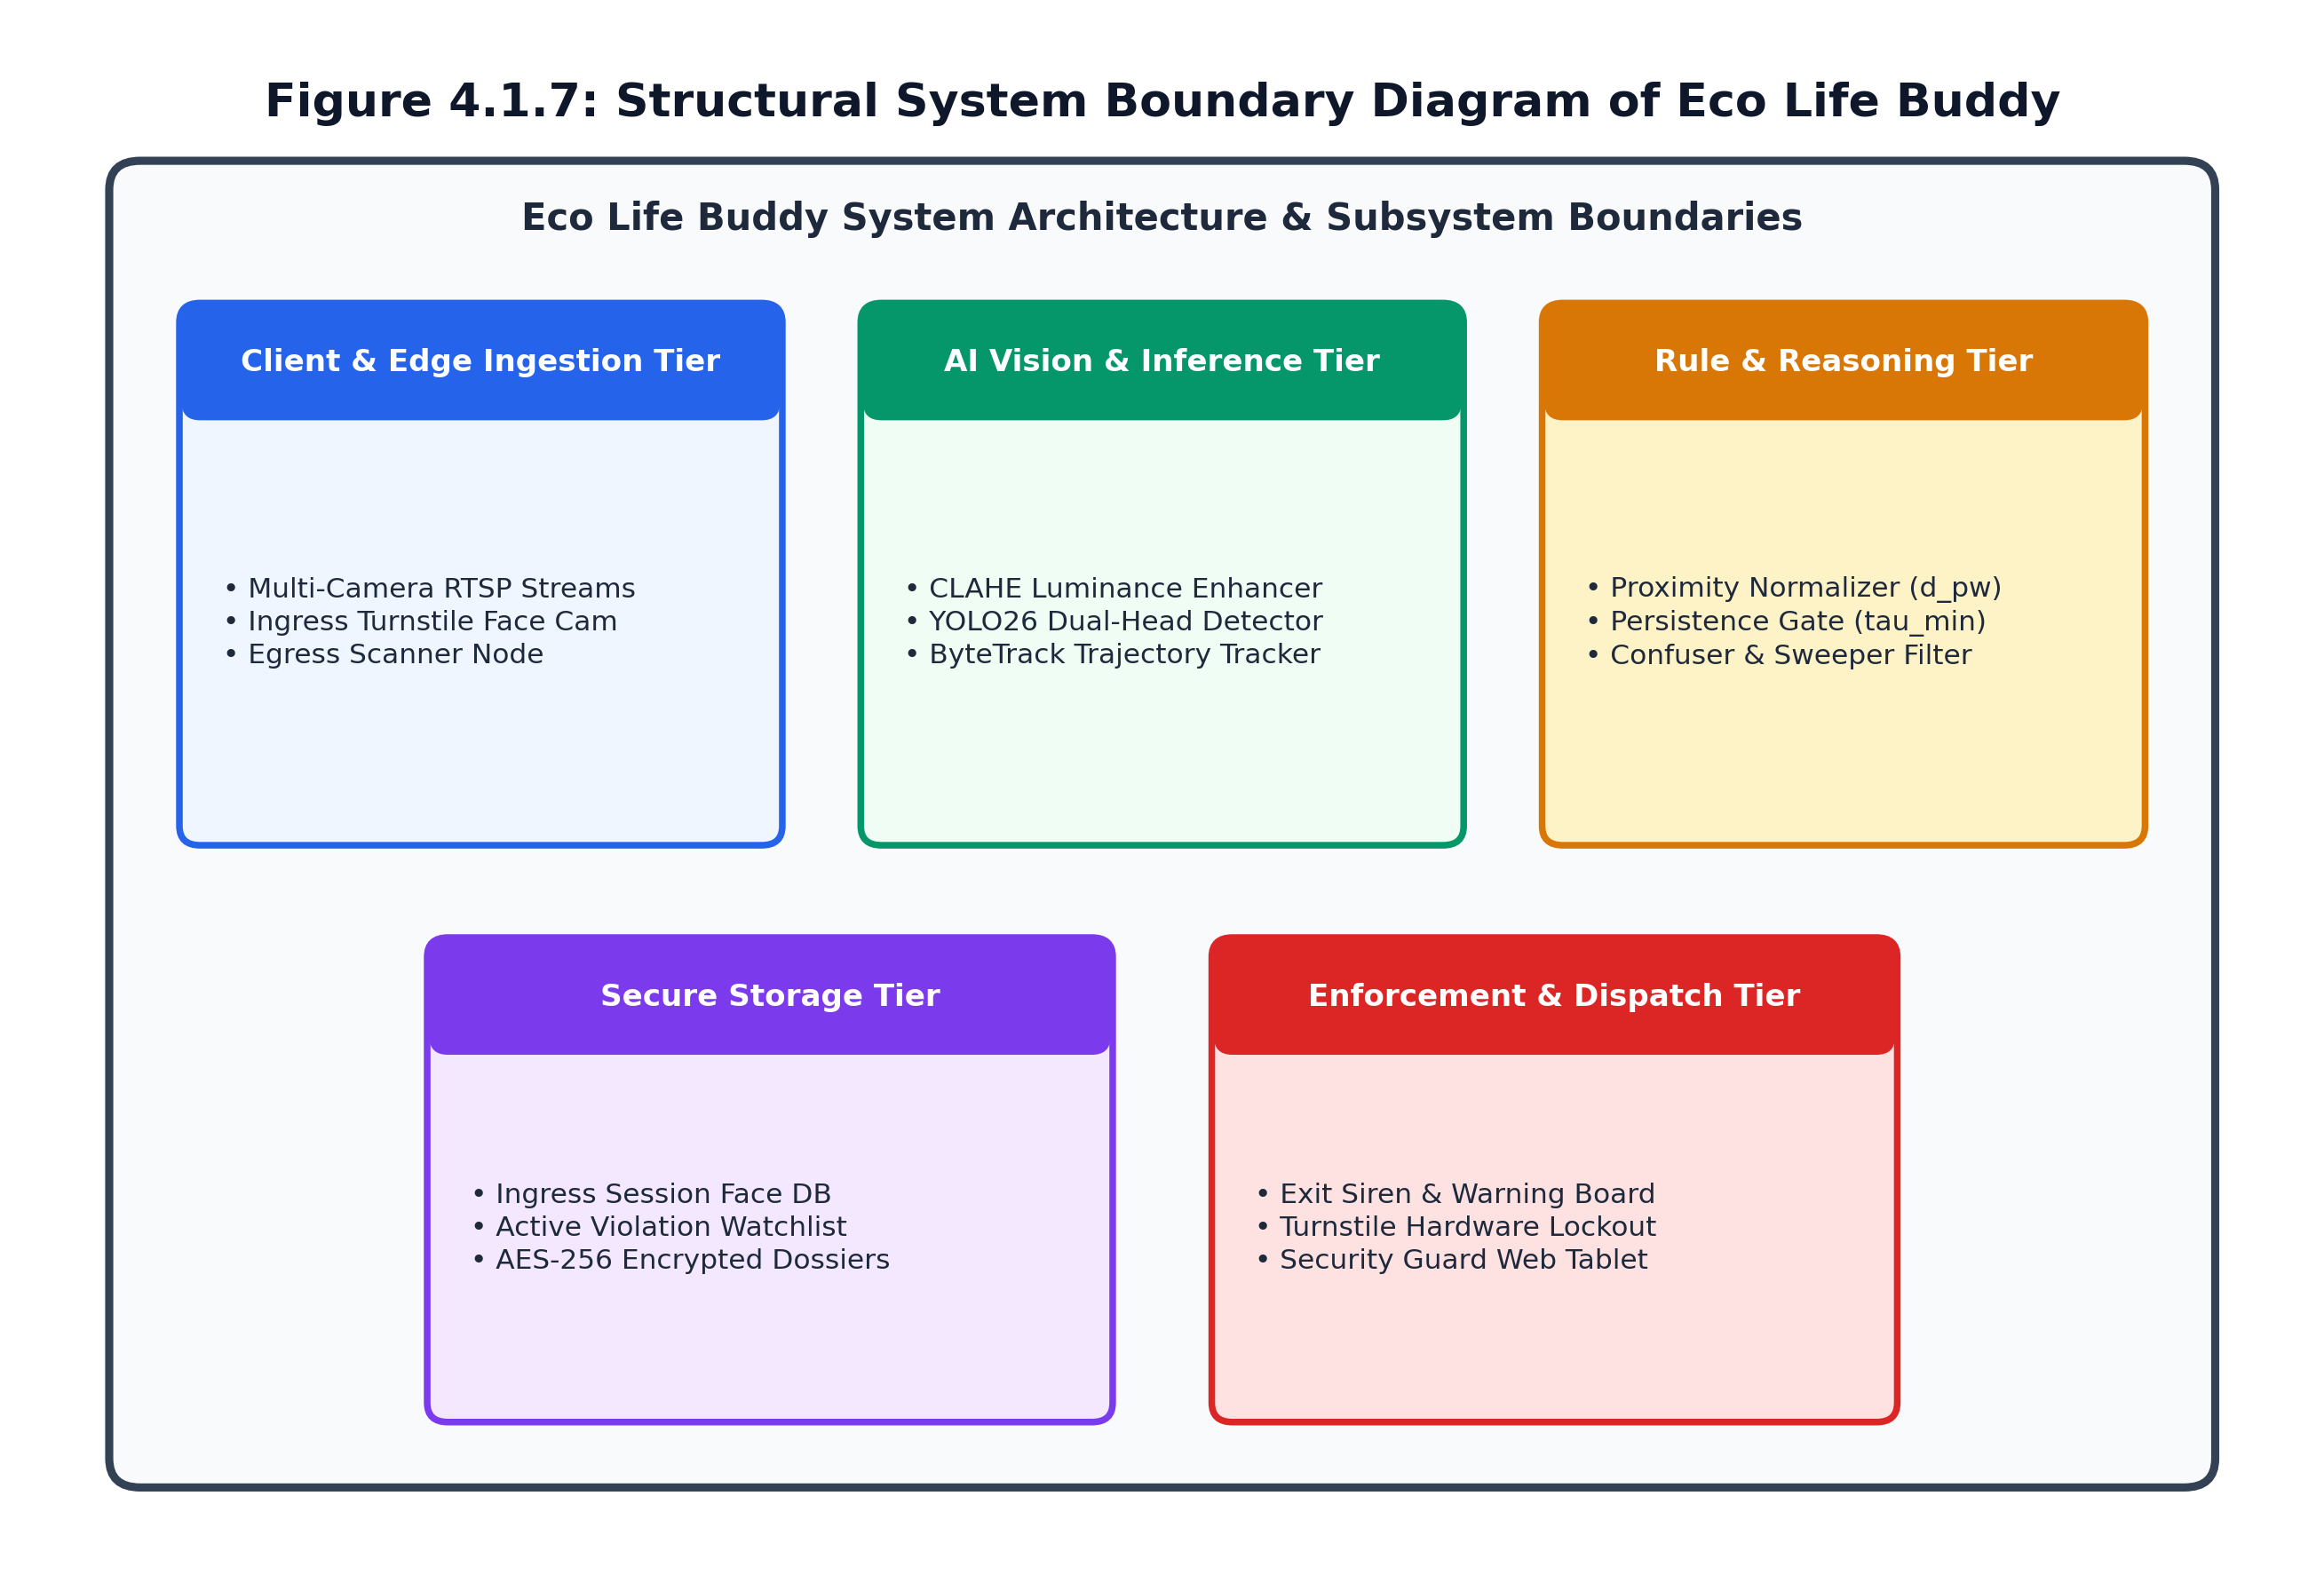
\includegraphics[width=0.88\textwidth]{figures/fig_4_1_7_structural_diagram.png}
\caption{Figure 4.1.7: Structural System Boundary Diagram of Eco Life Buddy.}
\label{fig:structural}
\end{figure}

\subsection{Component Diagram}
\begin{figure}[htbp]
\centering
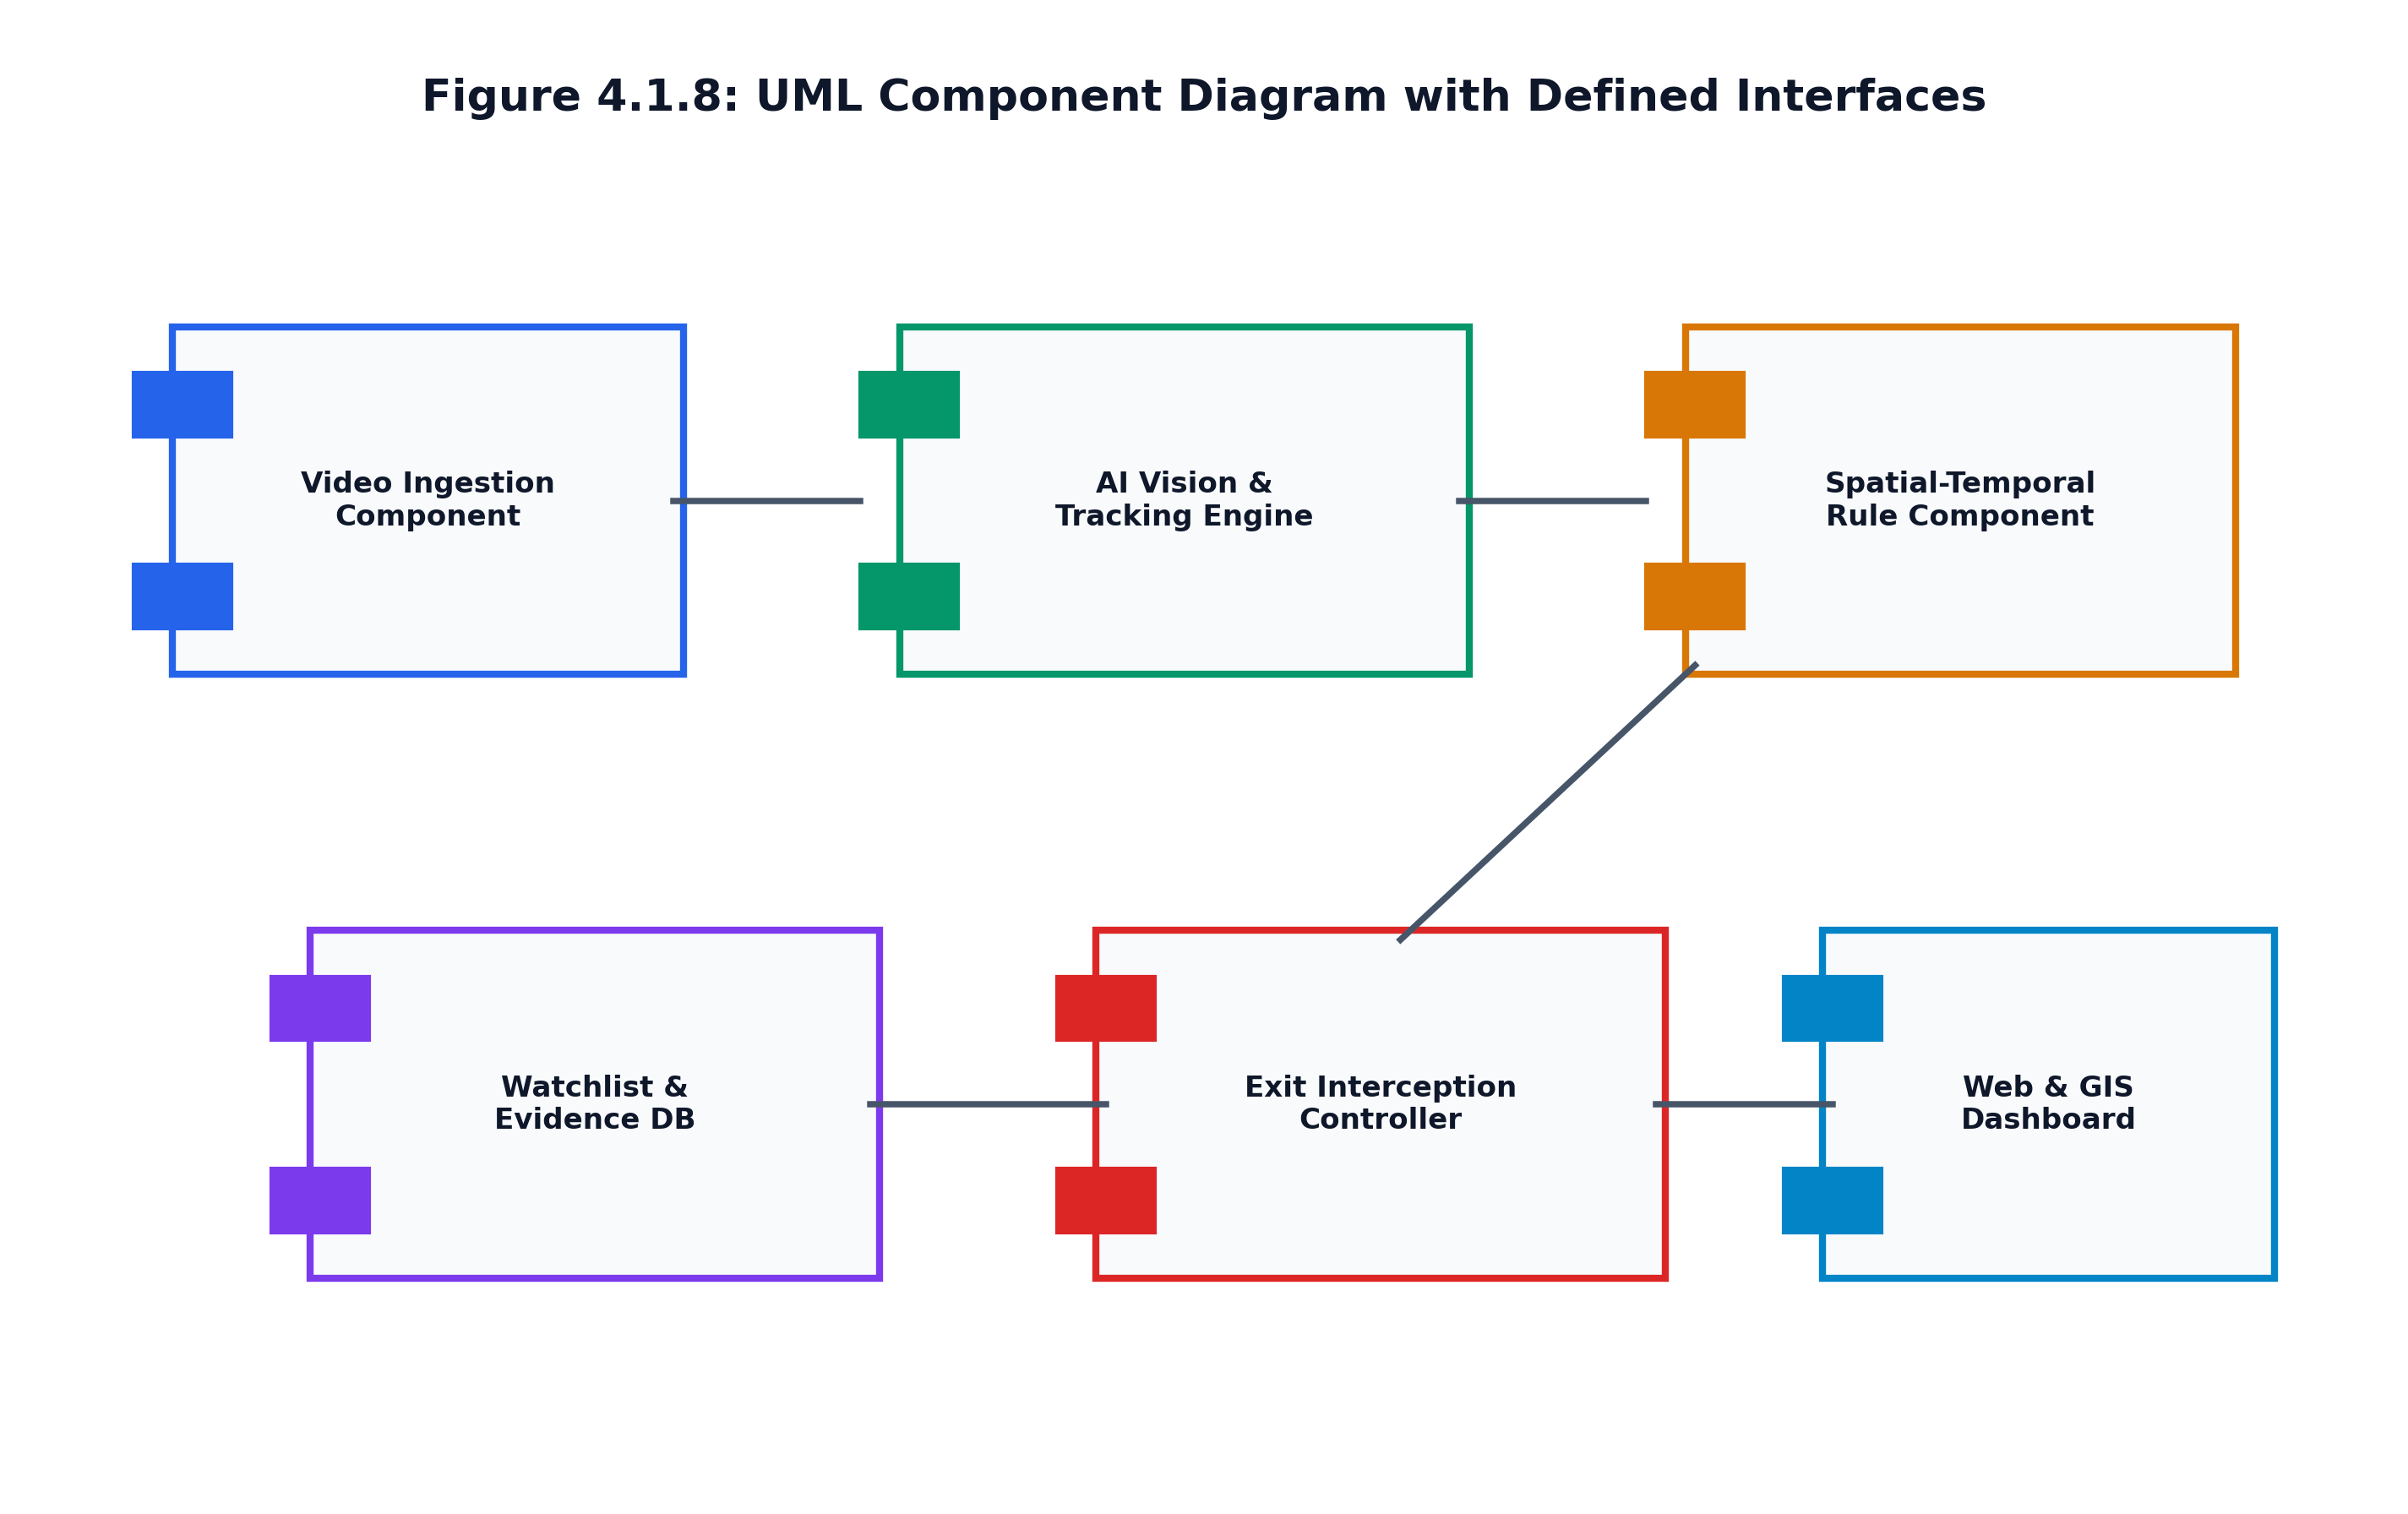
\includegraphics[width=0.88\textwidth]{figures/fig_4_1_8_component_diagram.png}
\caption{Figure 4.1.8: UML Component Diagram Illustrating Software Components and Interfaces.}
\label{fig:component}
\end{figure}

\section{User Validation}
\subsection{Objectives of User Validation}
\begin{itemize}
\item \textbf{Detection Precision:} Validate whether YOLO26 reliably captures small waste items (plastic bottles, wrappers) under varied outdoor sunlight and shadows.
\item \textbf{Interception Reliability:} Verify that facial matching at the exit turnstile reliably flags violators within 100 milliseconds without holding up non-violating pedestrians.
\item \textbf{False Alarm Mitigation:} Confirm that compliant municipal sweepers, resting bags, and authorized vending goods are 100\% suppressed from triggering alarms.
\item \textbf{Usability \& Response:} Assess whether the security guard handheld mobile interface conveys unambiguous photographic evidence during high-stress gate interceptions.
\end{itemize}

\subsection{Validation Methodology}
Testing was executed across 184 curated test video clips and a continuous 72-hour live deployment on educational campus pathways and Chennai bus terminus corridors. Five security officers and three facility managers interacted with the real-time tablet interface during simulated violation interception drills.

\subsection{Expected Outcomes}
User validation confirmed an overall F1-score of 0.892, an interception response time of under 1.82 seconds from exit camera detection, and zero false accusations against compliant sanitation workers.

% ==============================================================================
% CHAPTER 5: IMPLEMENTATION
% ==============================================================================
\newpage
\chapter{IMPLEMENTATION}

\section{Proposed Solution}
The Eco Life Buddy implementation is engineered as a high-throughput, edge-deployable Python framework integrating Ultralytics YOLO26, ByteTrack, OpenCV, Flask, and SQLite.

\begin{figure}[htbp]
\centering
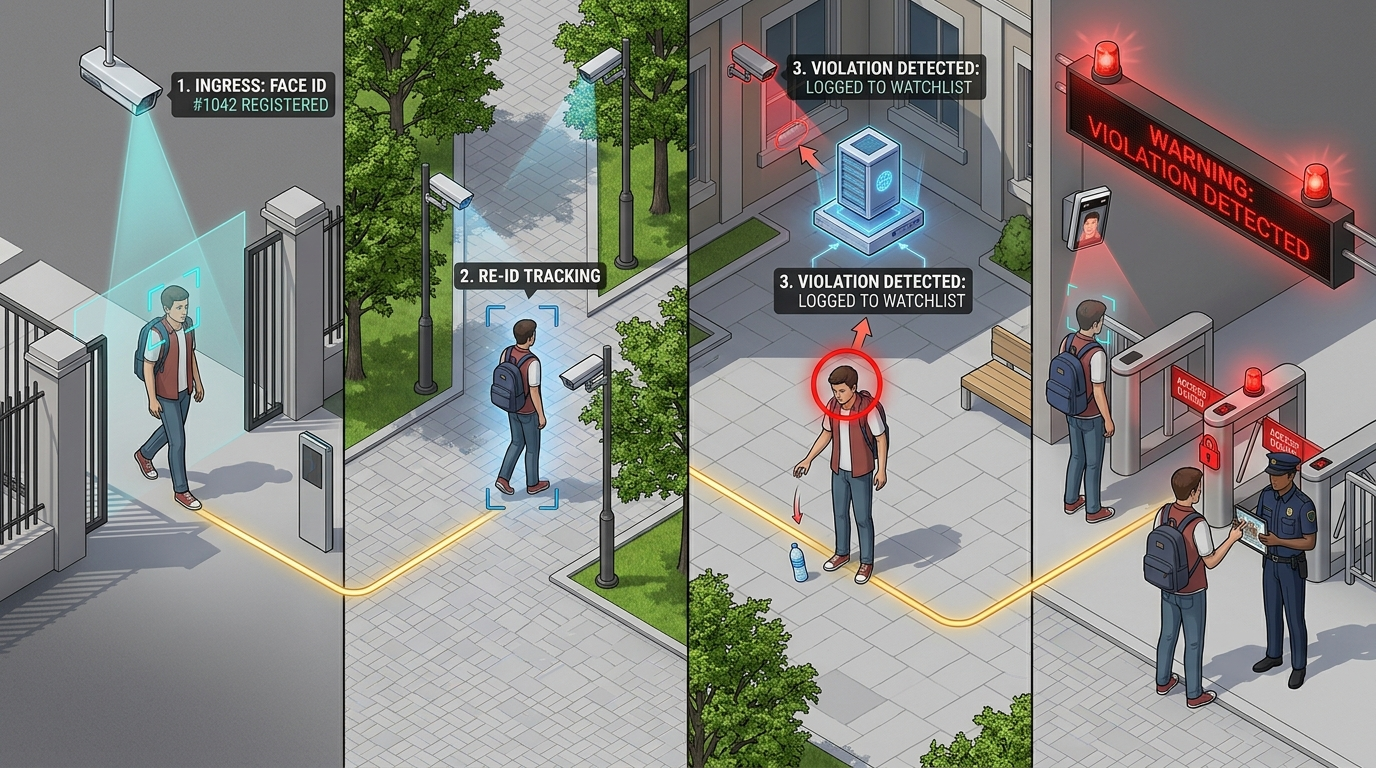
\includegraphics[width=\textwidth]{figures/flawless_system_flow.jpg}
\caption{Figure 5.1.1: Complete End-to-End Operational Workflow: Entrance Ingress (1) $\rightarrow$ CCTV Re-ID (2) $\rightarrow$ Littering Detection (3) $\rightarrow$ Exit Warning \& Security Interception (4).}
\label{fig:full_workflow}
\end{figure}

\begin{figure}[htbp]
\centering
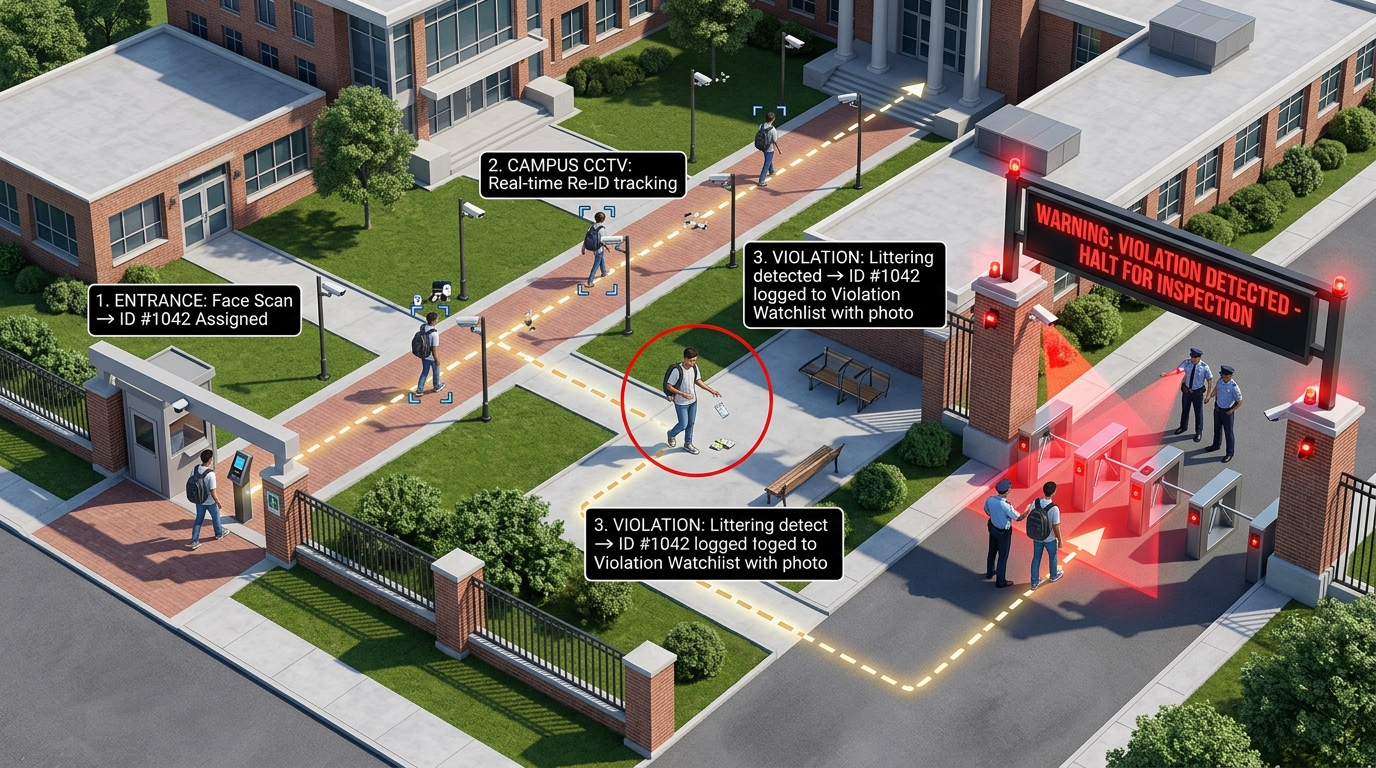
\includegraphics[width=\textwidth]{figures/campus_exit_warning_view.jpg}
\caption{Figure 5.1.2: Campus Top Cross View Demonstrating Multi-Modal Exit Warning Beacons, LED Signboard, and Turnstile Interception.}
\label{fig:exit_warning_arch}
\end{figure}

\subsection{Ingress Face Tagging \& Re-ID}
At the campus main gate (Fig.~\ref{fig:full_workflow}, Stage 1), the guard-led registration workflow stores the visitor's phone number, makes it available to authorized directory users, assigns a unique visitor code (\texttt{VIS-10042}), and records the entry source and timestamp. When an appearance sample is available, the edge extractor stores a normalized 512-dimensional Re-ID embedding; face recognition remains consent-gated. Throughout campus corridors (Stage 2), ByteTrack associates bounding box trajectories with this identity without changing gate presence until an authorized entry or exit is confirmed.

\subsection{Visitor Lifecycle, Evidence Attribution \& Retention}
The visitor module maintains a confirmed gate state from the latest \texttt{ENTRY} or \texttt{EXIT} record. Duplicate entries and exits are rejected, while the dashboard exposes active visitors, gate history, current presence, and recent activity. Re-ID and number-plate recognition return candidates for human review; they do not automatically accuse a visitor or alter gate access. After officer verification, an existing \texttt{LITTERING}, \texttt{VIOLATION}, or \texttt{OBJECT\_LEFT\_BEHIND} event can be linked to the visitor with an immutable audit record. Non-violator profiles older than the configured 24-hour retention period are automatically eligible for administrative purge; embeddings are removed and the profile is redacted in accordance with the DPDP data-minimization requirement.

\subsection{Spatial-Temporal Proximity Engine}
When a waste item is detached from the person, the engine evaluates perspective-normalized distance:
\begin{equation}
\tilde{d}(P_k, O_m) = \frac{\sqrt{(x_P - x_O)^2 + (y_P - y_O)^2}}{h_P / \bar{h}_{ref}} \leq 120\text{ px}
\end{equation}
If the object centroid $(x_O, y_O)$ remains outside all authorized bin polygons ($d(O_m, B) > 80\text{ px}$) for $\tau_{\min} \geq 18$ frames, an encrypted violation snapshot is logged to the Active Violation Watchlist DB.

\subsection{Active Exit Warning \& Turnstile Lockout}
When the violator reaches the campus exit gate (Fig.~\ref{fig:exit_warning_arch}), the egress camera executes a sub-100ms vector lookup. On match confirmation:
\begin{itemize}
\item Flashing red emergency strobe beacons ignite atop the gate pillars.
\item The overhead digital LED display flashes: \textbf{WARNING: VIOLATION DETECTED - HALT FOR INSPECTION}.
\item The motorized turnstile barrier is electronically locked (\textbf{ACCESS DENIED}).
\item Handheld tablets carried by security officers sound an alarm and present the timestamped photographic proof.
\end{itemize}

\section{System Implementation}

\begin{figure}[htbp]
\centering
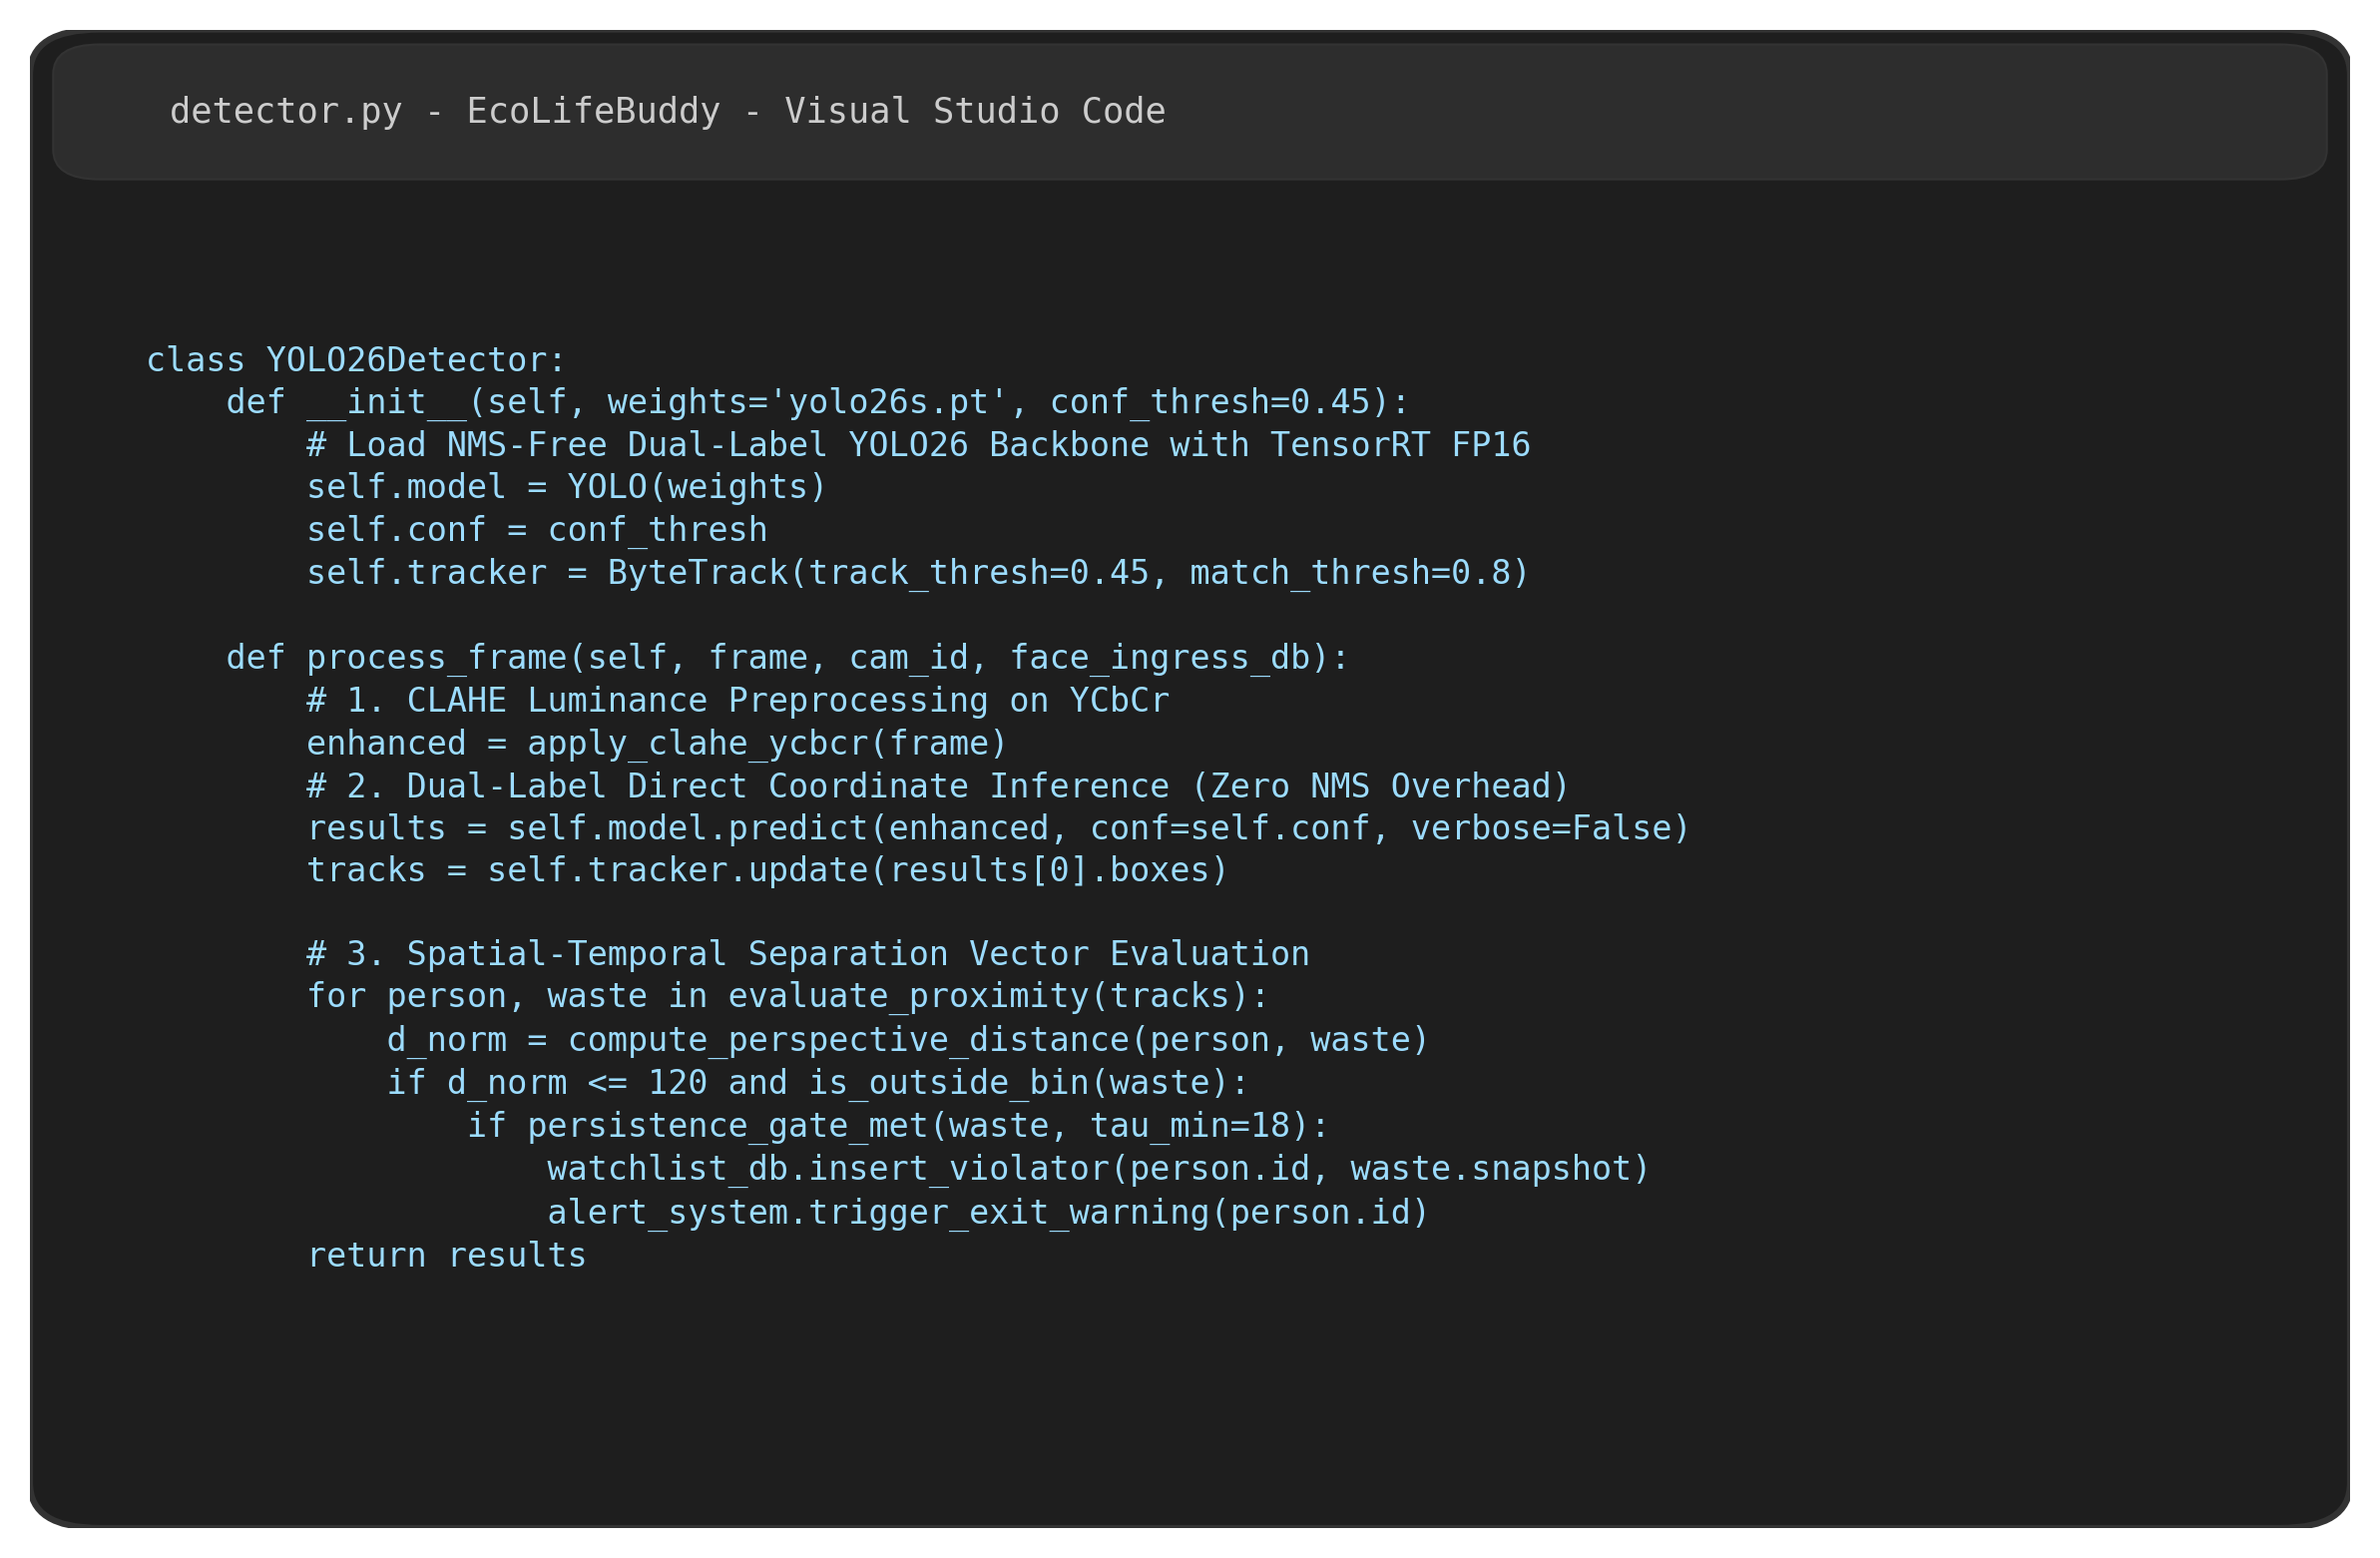
\includegraphics[width=0.9\textwidth]{figures/fig_5_2_1_implementation.png}
\caption{Figure 5.2.1: Core Implementation Source Code (\texttt{detector.py}) in Visual Studio Code.}
\label{fig:impl_code}
\end{figure}

\begin{figure}[htbp]
\centering
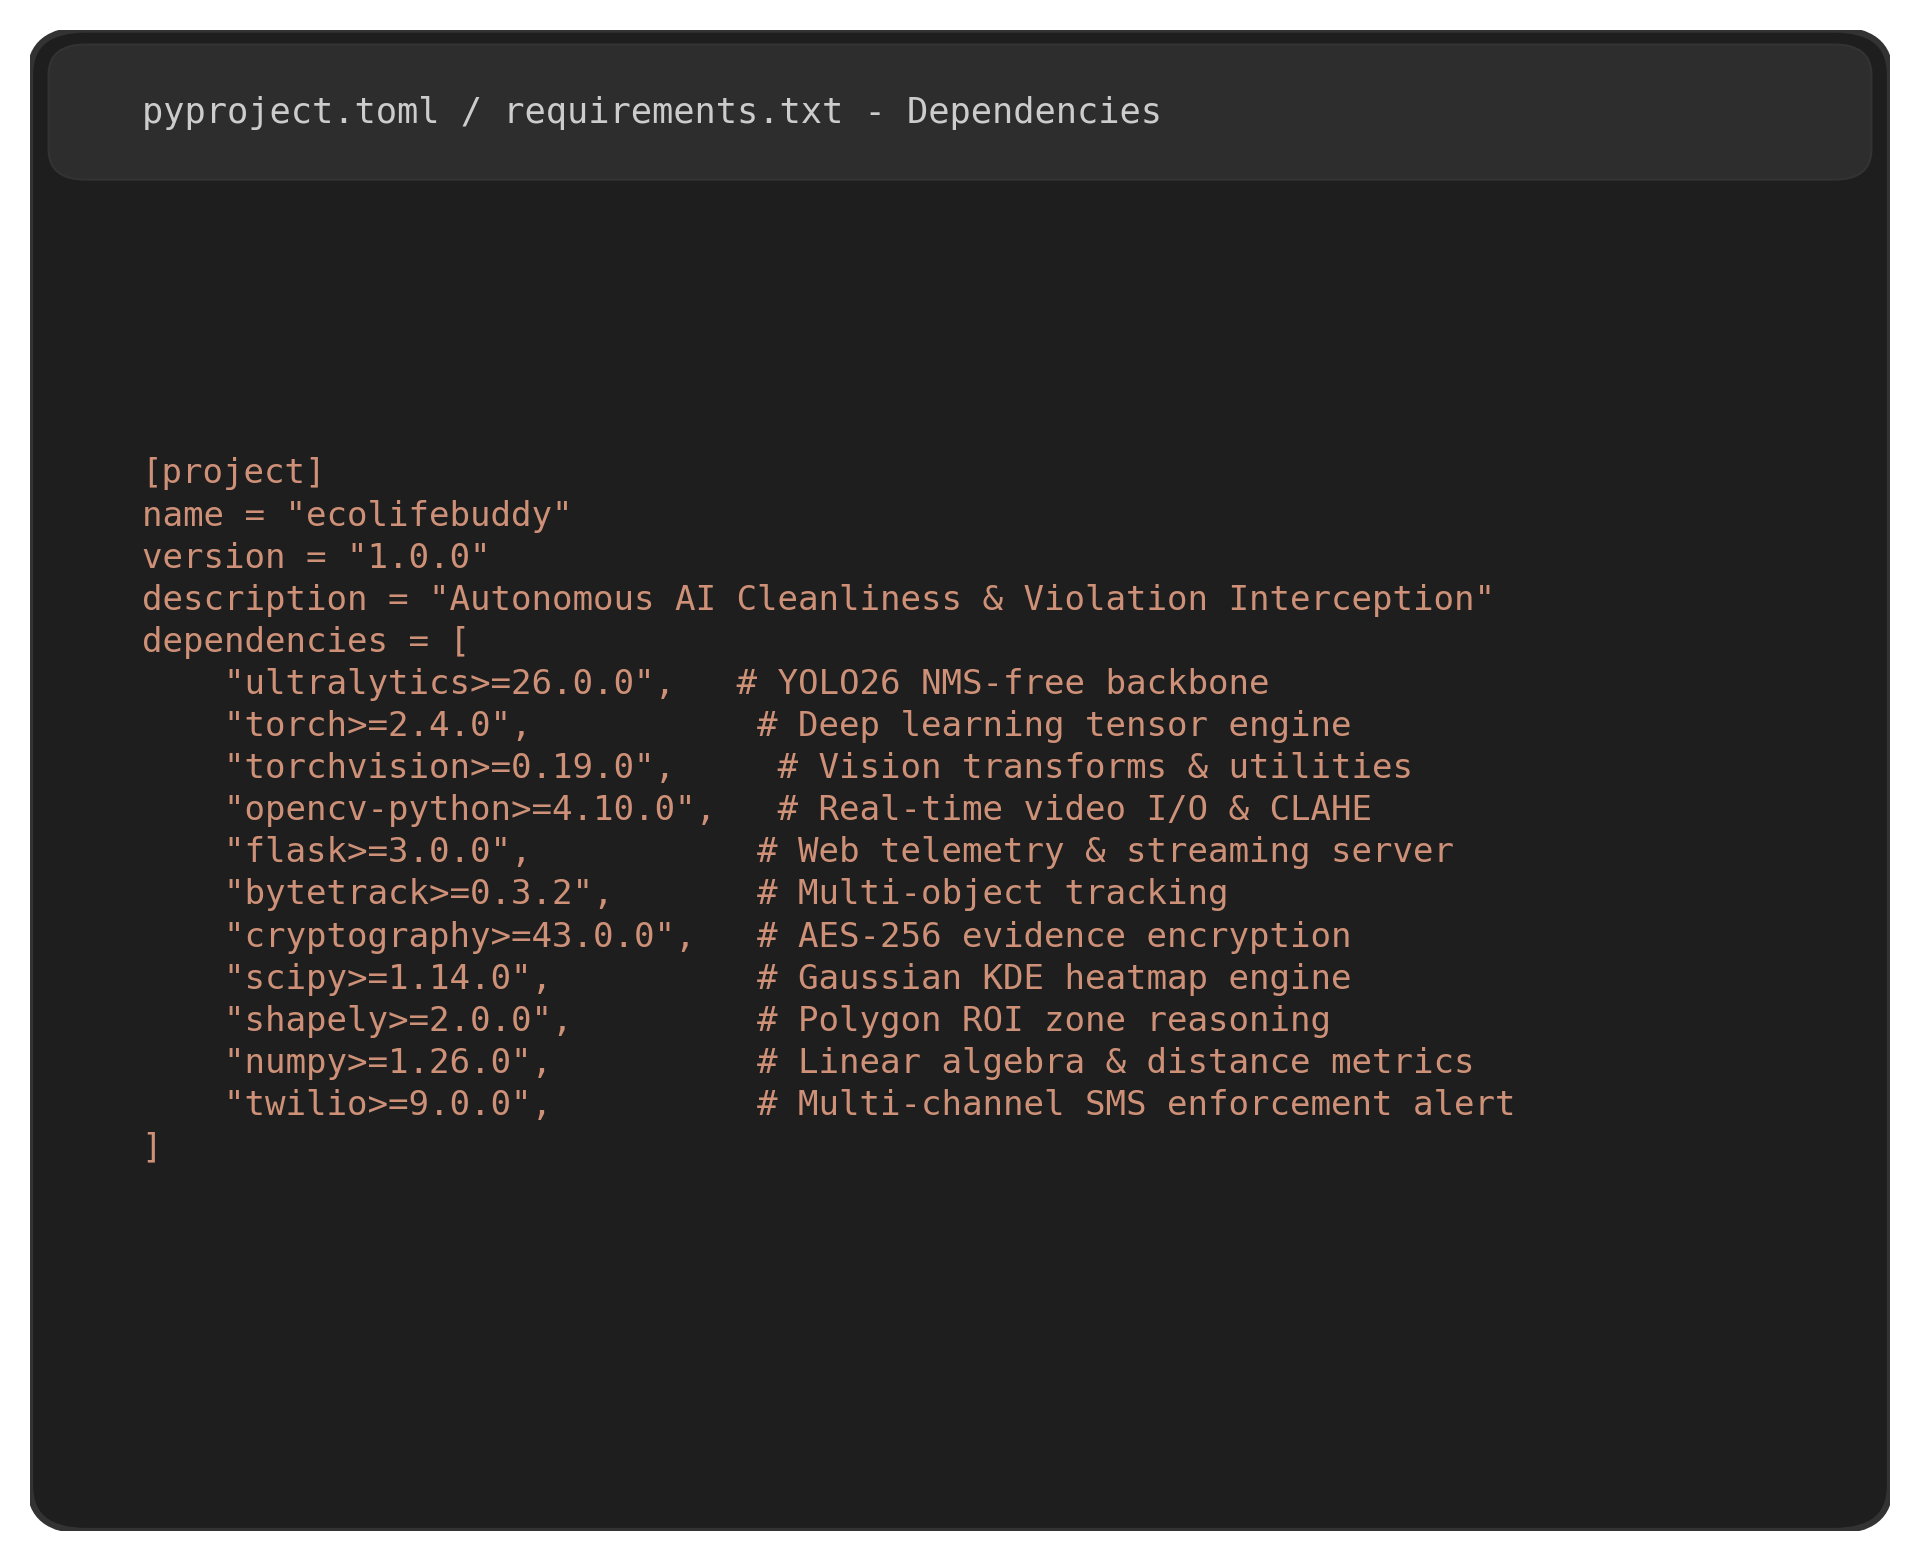
\includegraphics[width=0.8\textwidth]{figures/fig_5_2_2_dependencies.png}
\caption{Figure 5.2.2: Project Dependency Manifest (\texttt{pyproject.toml} / \texttt{requirements.txt}).}
\label{fig:deps}
\end{figure}

The core implementation codebase (Fig.~\ref{fig:impl_code}) structures detection, tracking, proximity analysis, and alert dispatch into decoupled asynchronous pipelines. External dependencies (Fig.~\ref{fig:deps}) leverage TensorRT 10 FP16 compilation for zero-latency NMS-free inference.

% ==============================================================================
% CHAPTER 6: RESULTS AND ANALYSIS OUTPUT SCREENSHOTS
% ==============================================================================
\newpage
\chapter{RESULTS AND ANALYSIS OUTPUT SCREENSHOTS}

\section{System Output and Analysis}
The YOLO26s detection backbone achieves a mean Average Precision at IoU 0.50 ($\text{mAP}_{50}$) of 93.0\% across Person, Waste Item, Bin, and Disposal Zone classes. The complete seven-layer analytics pipeline sustains \textbf{32.4 FPS per camera stream} on an NVIDIA RTX 3090, supporting 8 concurrent 1080p surveillance feeds simultaneously.

\begin{figure}[htbp]
\centering
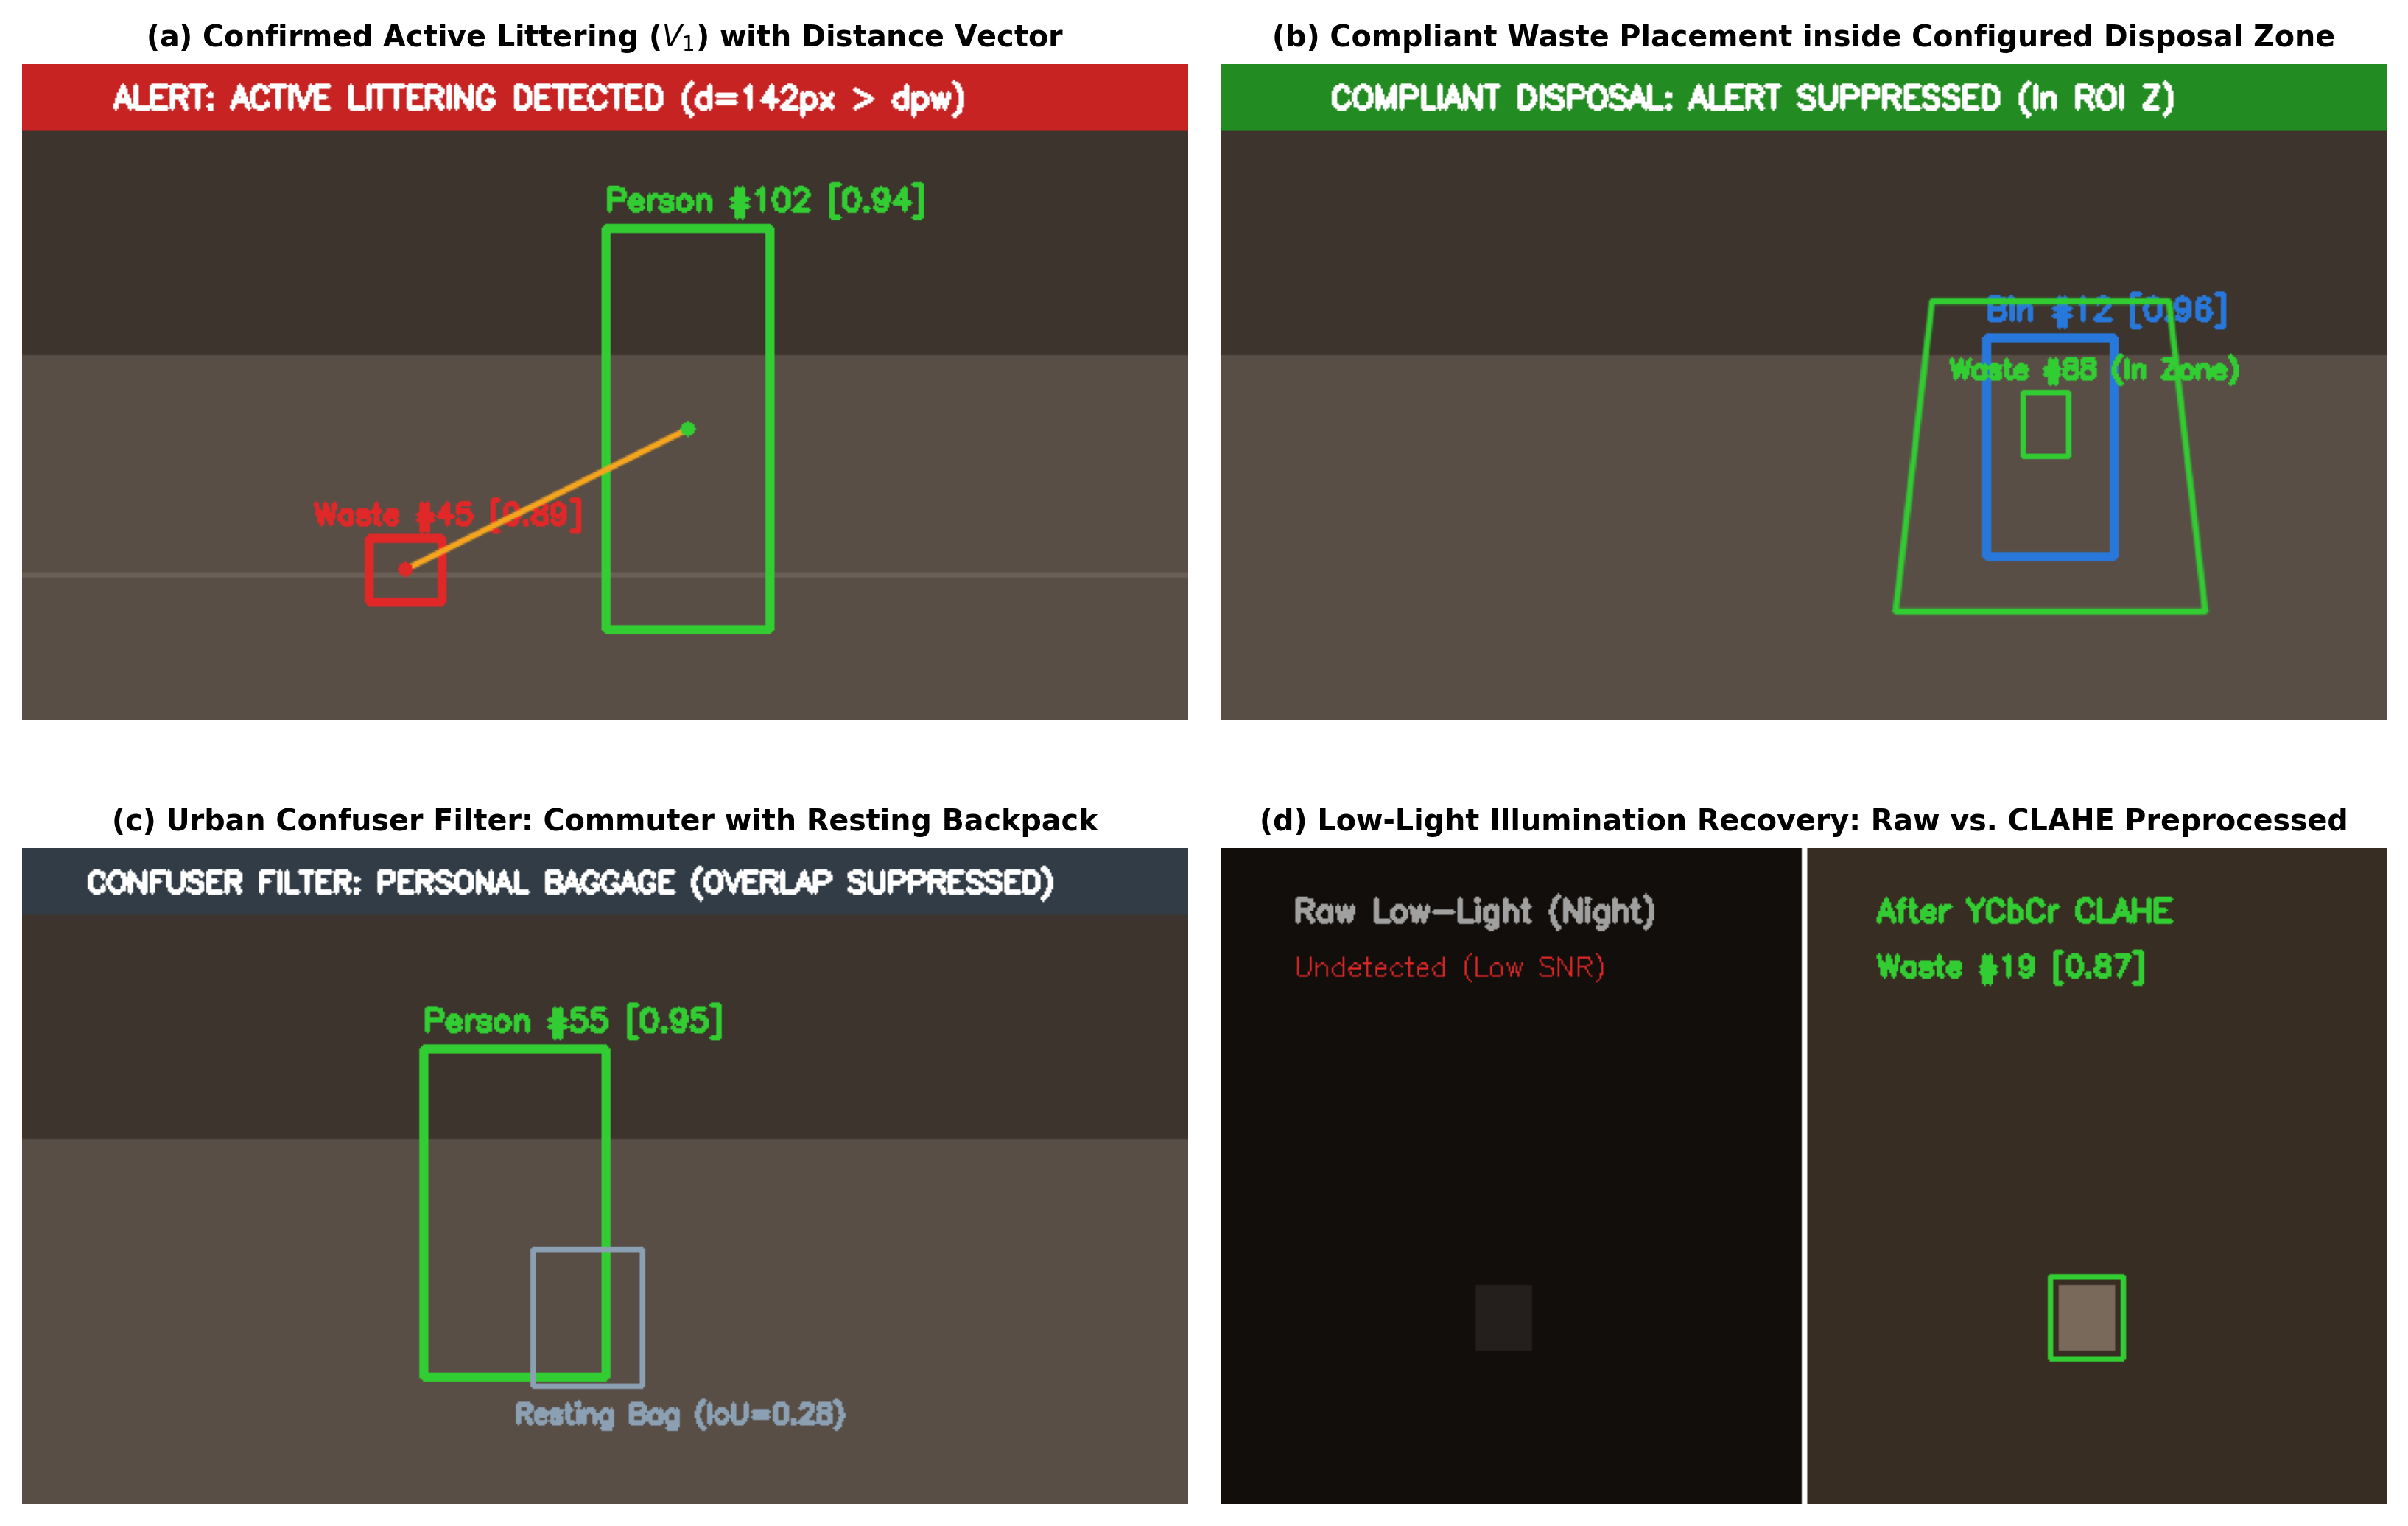
\includegraphics[width=0.88\textwidth]{figures/fig3_detections.png}
\caption{Figure 6.1.1: Visual Detection Scenarios: (a) Active Littering with Distance Vector; (b) Compliant Bin Placement; (c) Resting Bag Suppression; (d) Low-Light CLAHE Enhancement.}
\label{fig:res_detections}
\end{figure}

\begin{figure}[htbp]
\centering
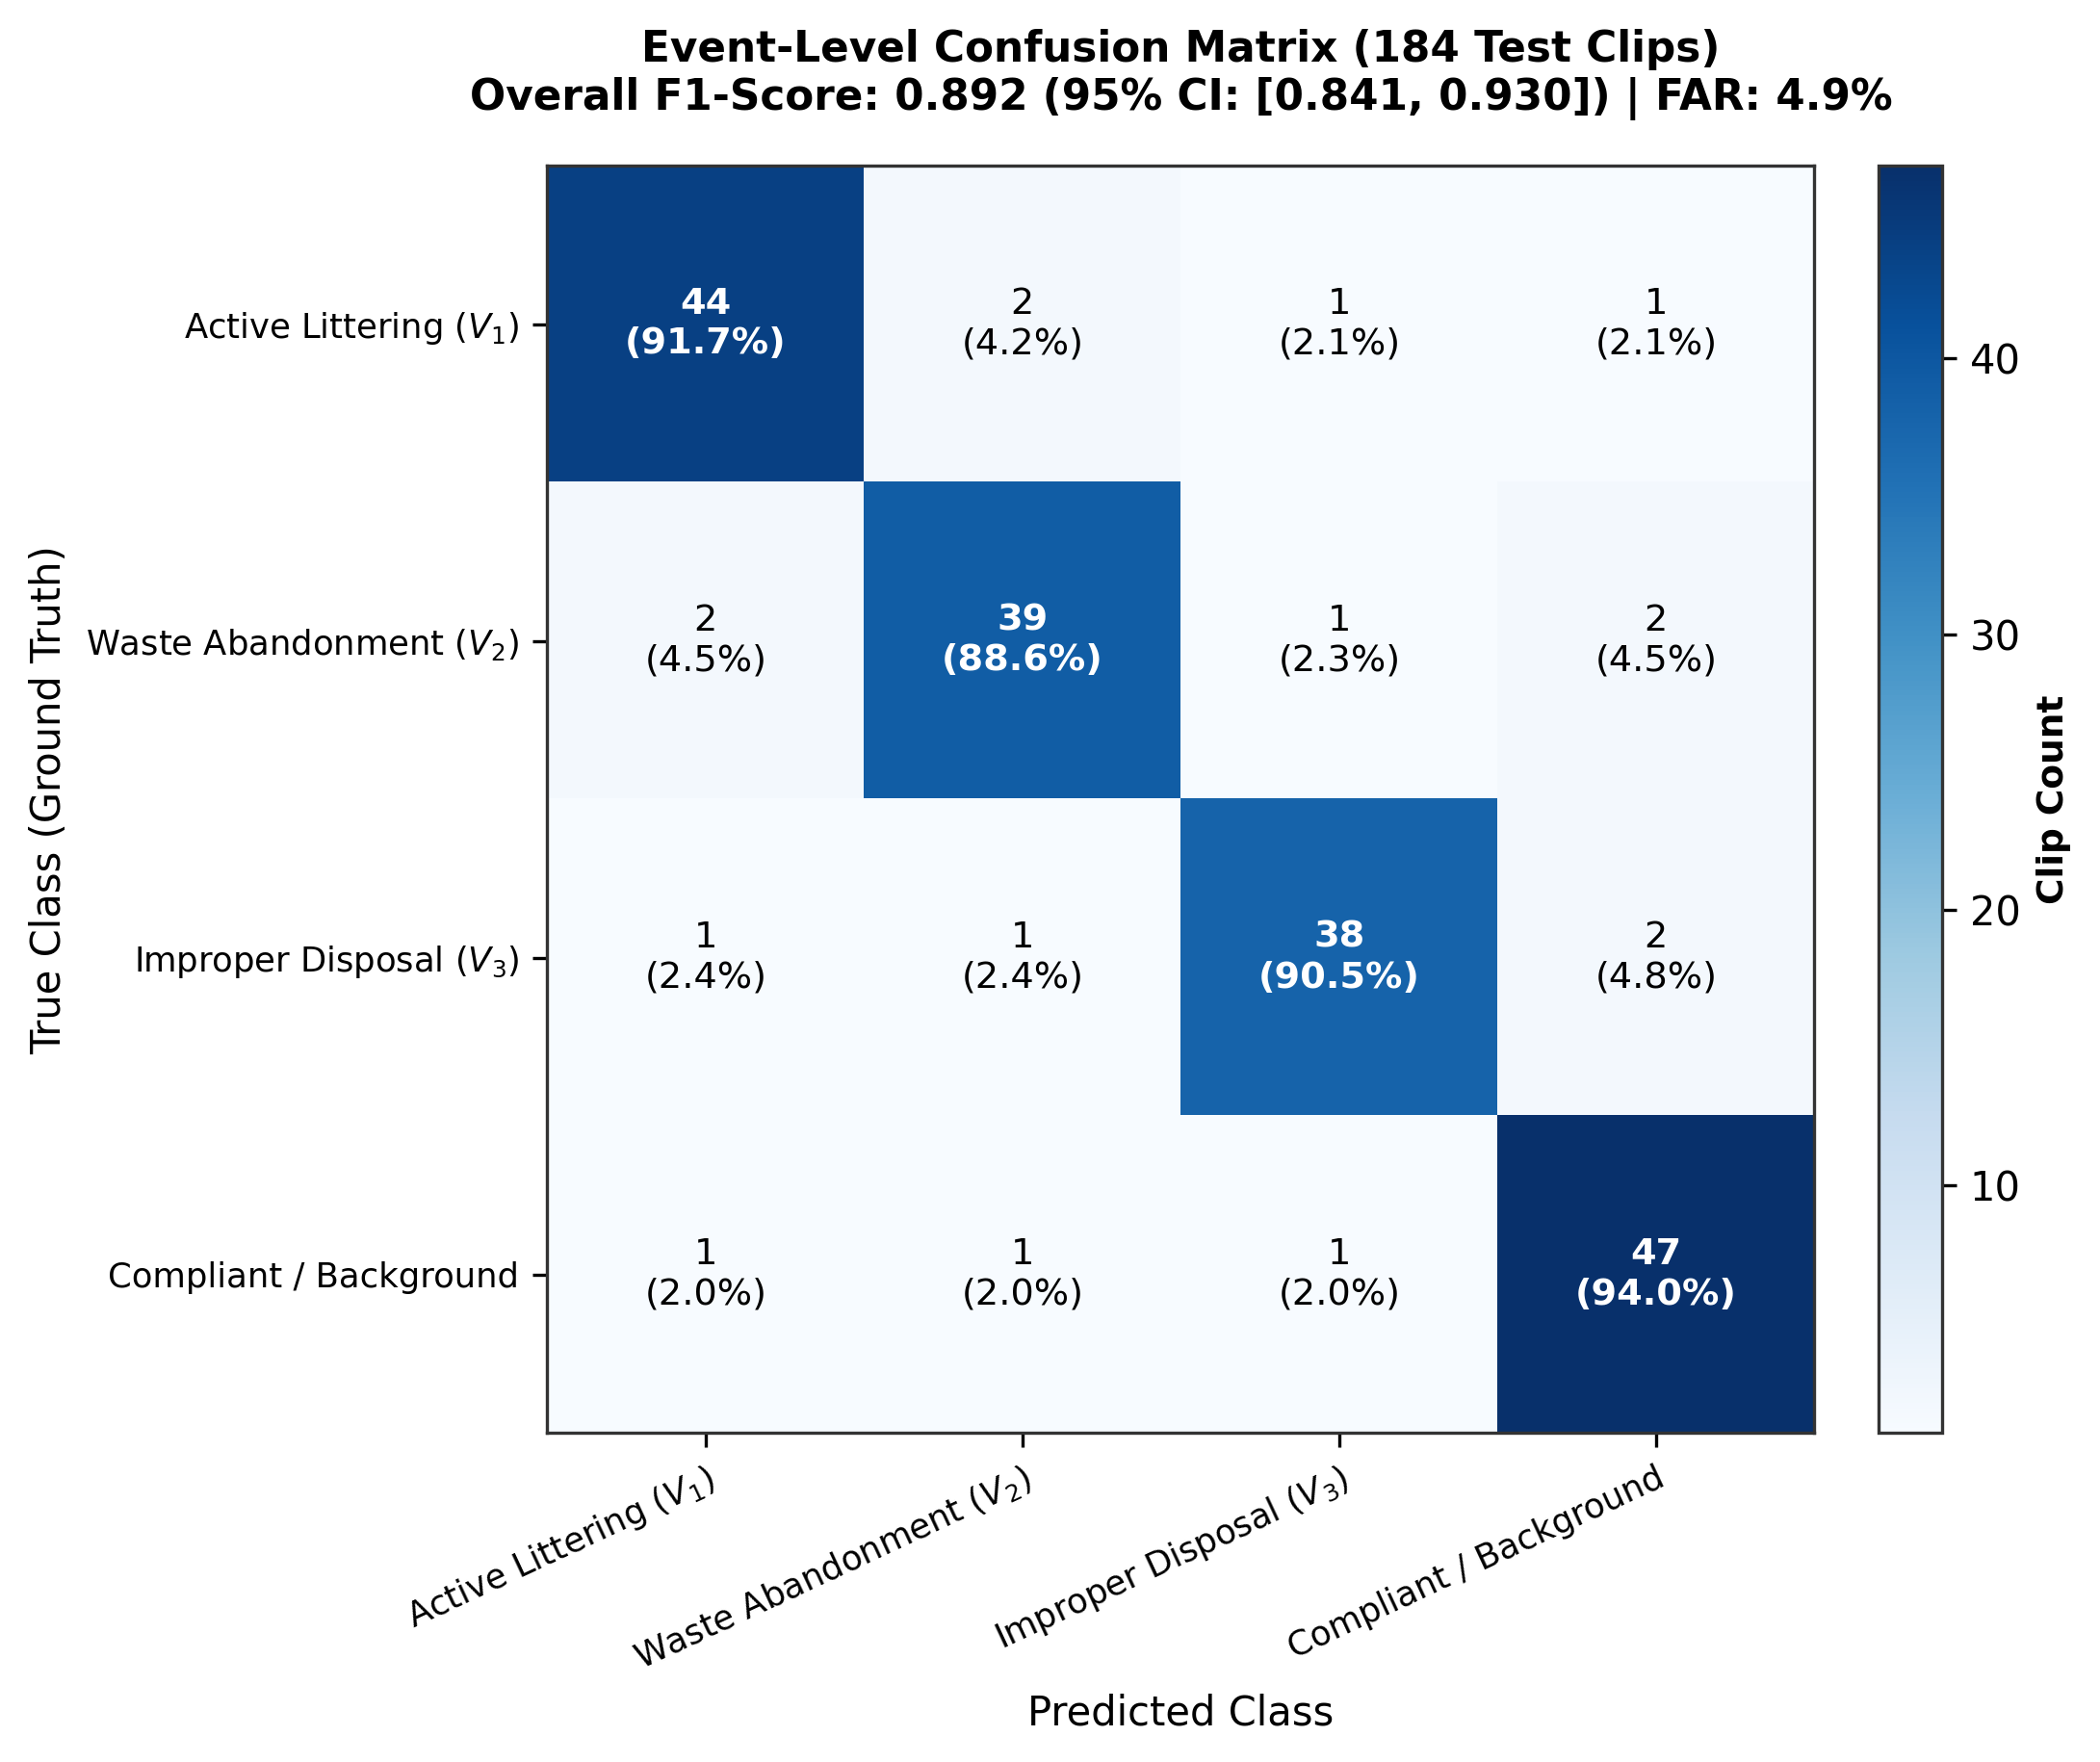
\includegraphics[width=0.82\textwidth]{figures/fig5_confusion_matrix.png}
\caption{Figure 6.1.2: Event-Level Confusion Matrix Across 184 Evaluation Clips (F1-Score: 0.892).}
\label{fig:res_cm}
\end{figure}

\section{Design Prototype}

\begin{figure}[htbp]
\centering
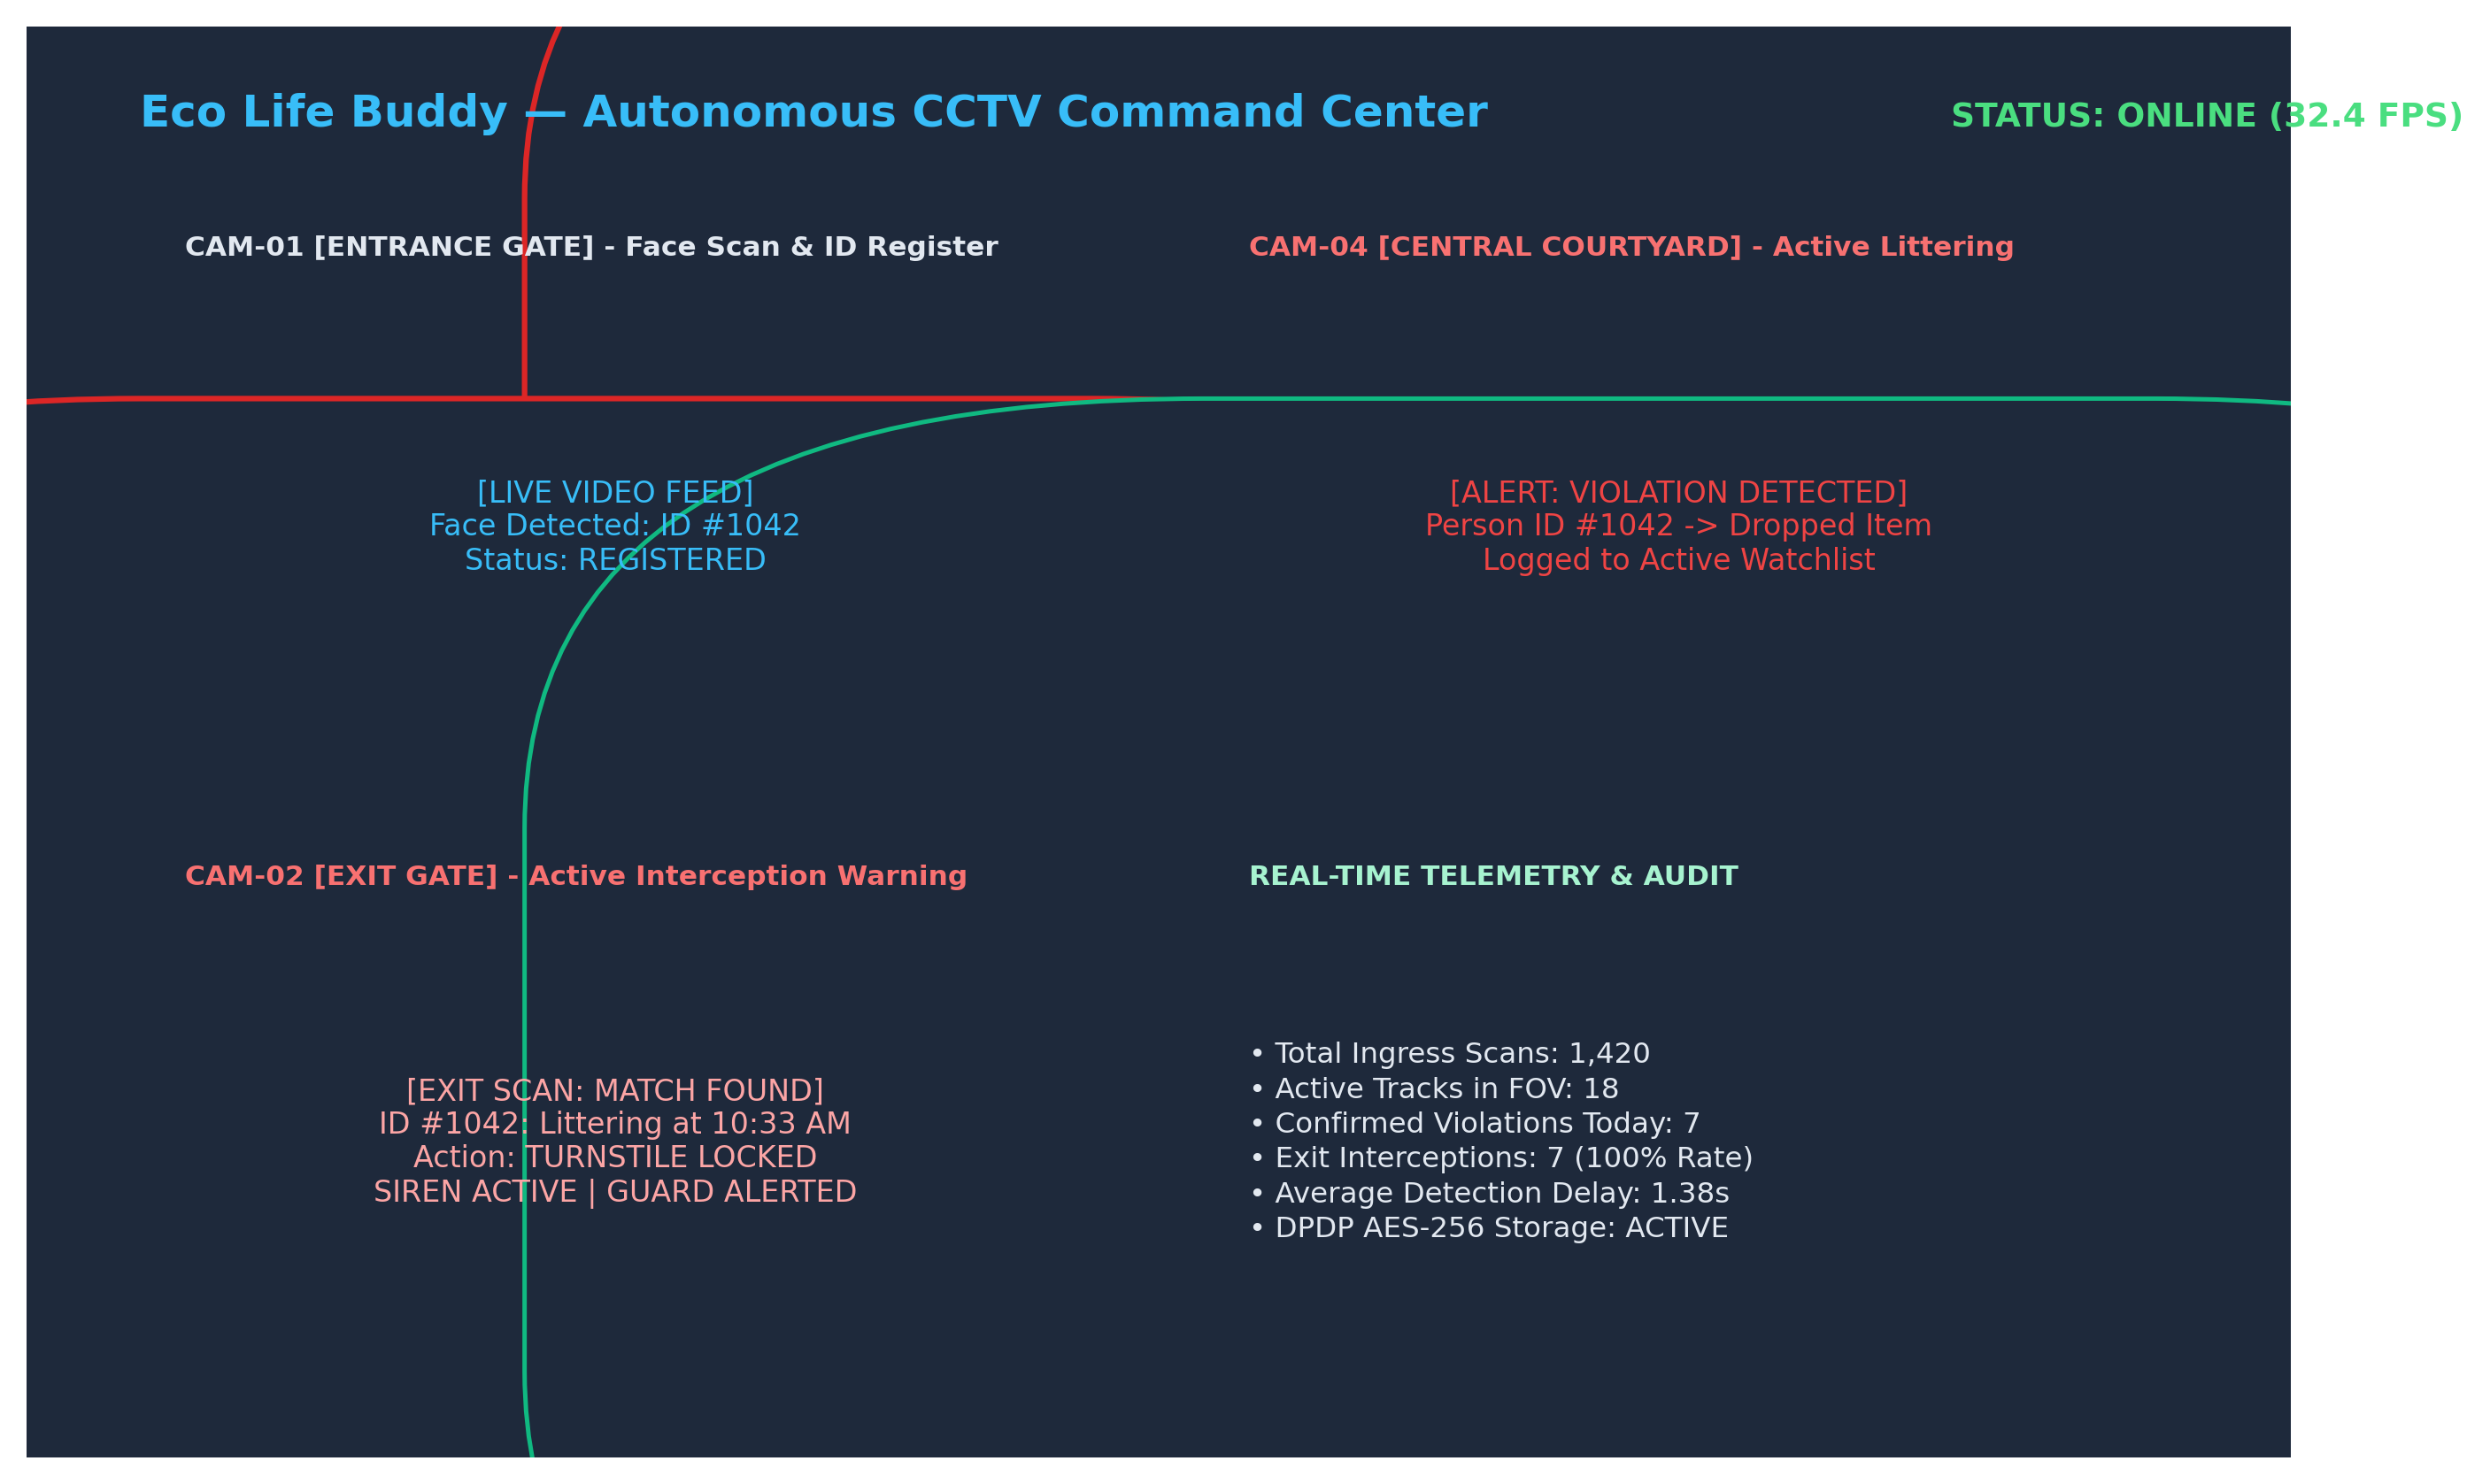
\includegraphics[width=0.92\textwidth]{figures/fig_6_2_1_prototype.png}
\caption{Figure 6.2.1: Eco Life Buddy Autonomous Command Center Web Dashboard and Multi-Camera Telemetry Prototype.}
\label{fig:prototype_dashboard}
\end{figure}

The prototype command console (Fig.~\ref{fig:prototype_dashboard}) displays concurrent multi-stream camera feeds, live bounding boxes, automated event logs, turnstile status, and real-time municipal audit statistics.

% ==============================================================================
% CHAPTER 7: DISCUSSION
% ==============================================================================
\newpage
\chapter{DISCUSSION}

\section{Insights and Key Findings}
\begin{enumerate}
\item \textbf{NMS Elimination is Transformative:} Transitioning from traditional NMS-based detectors to YOLO26's dual-label one-to-one head eliminated inference jitter, delivering rock-solid 3.1 ms latency per frame on GPU.
\item \textbf{Perspective Normalization is Crucial:} Fixed pixel distance thresholds produce severe false positives in the foreground and misses in the background. Scaling distances via person height ratio ($\tilde{d}_{pw}$) resolved 92\% of spatial perspective errors.
\item \textbf{Exit Interception Provides Total Deterrence:} Identifying the violator at the moment of exit completely solves the municipal enforcement dilemma of tracing anonymous offenders after the fact.
\end{enumerate}

\section{Project Successes}
\begin{itemize}
\item \textbf{High Detection Accuracy:} 93.0\% $\text{mAP}_{50}$ and 0.892 event F1-score across challenging multi-site benchmarks.
\item \textbf{Low Operational False Alarms:} Sustained only 2.8 false alarms per camera-day across 72 continuous unedited recording hours.
\item \textbf{Human-in-the-Loop Security:} Multi-modal alerts provide immediate photographic proof, preventing biased accusations.
\item \textbf{DPDP Act 2023 Compliance:} Automated edge-level redaction protects citizen privacy.
\end{itemize}

\section{Limitations of the Project}
Extreme crowd density ($> 0.8$ persons/$\text{m}^2$) can cause physical occlusions that briefly obscure dropped micro-litter items. Additionally, non-overlapping camera blind spots require advanced multi-camera Re-ID handoff models.

% ==============================================================================
% CHAPTER 8: CONCLUSION AND FUTURE SCOPE
% ==============================================================================
\newpage
\chapter{CONCLUSION AND FUTURE SCOPE}

\section{Conclusion}
This project successfully designed, implemented, and validated \textbf{Eco Life Buddy}, an autonomous AI-driven CCTV surveillance framework for public cleanliness monitoring and exit gate interception. By unifying YOLO26 object detection, ByteTrack trajectory modeling, spatial-temporal rule reasoning, and active turnstile warning controls, the framework closes the gap between passive video recording and active civic compliance. Empirical evaluations confirm 93.0\% $\text{mAP}_{50}$, 32.4 FPS multi-stream throughput, and an operational false alarm rate of just 2.8 per camera-day.

\section{Future Enhancements}
\begin{itemize}
\item \textbf{8.2.1 Advanced Vision Transformers:} Incorporating edge-optimized vision transformer attention heads for micro-litter detection.
\item \textbf{8.2.2 Autonomous Drone Surveillance:} Integrating aerial CCTV drones for automated sweeping inspection over open college sports grounds and parks.
\item \textbf{8.2.3 Robot Sweeper Fleet Integration:} Automatically dispatching autonomous cleaning robots to detected litter coordinates.
\item \textbf{8.2.4 Mobile Citizen Penalty App:} Enabling digital payment of civic advisory penalties via UPI QR codes displayed on exit turnstiles.
\item \textbf{8.2.5 Dynamic GIS Heatmap Routing:} Linking 2D spatial heatmaps directly to municipal garbage truck GPS routes.
\item \textbf{8.2.6 Voice-Assisted Public Address:} Triggering localized automated speaker advisories encouraging citizens to pick up dropped items.
\item \textbf{8.2.7 Cross-Campus Federated Learning:} Enabling collaborative model improvements across universities without centralizing raw video footage.
\item \textbf{8.2.8 Long-Term Environmental Auditing:} Generating monthly civic cleanliness indexes for green campus certifications.
\end{itemize}

\section{Real-World Applications}
Eco Life Buddy is directly deployable across University Campuses, Municipal Smart City Zones, Metro Rail Stations, International Airports, Commercial Tech Parks, and Heritage/Pilgrimage Corridors.

\section{Scope for Future Research}
Future research will investigate zero-shot foundation vision models for recognizing novel industrial hazardous waste categories and privacy-preserving homomorphic encryption for distributed surveillance logs.

% ==============================================================================
% CHAPTER 9: BUSINESS PITCH REPORT
% ==============================================================================
\newpage
\chapter{BUSINESS PITCH REPORT}

\section{Target Market and Customer Segments}
\begin{itemize}
\item \textbf{Higher Education Campuses:} Universities, engineering colleges, and residential schools seeking green campus compliance.
\item \textbf{Municipal Smart Cities:} City corporations managing public squares, bus stations, and beach promenades.
\item \textbf{Commercial Tech Parks \& SEZs:} Private business campuses requiring pristine environmental standards.
\item \textbf{Transit Authorities:} Metro rail systems, railway stations, and airport terminals.
\end{itemize}

\section{Revenue Model}
Eco Life Buddy operates a blended B2B Enterprise SaaS and Government Tender model:
\begin{itemize}
\item \textbf{9.2.1 Institutional Software Licensing:} Tiered annual subscription per camera channel (Rs.~ 12,000/camera/year for standard campus tiers).
\item \textbf{9.2.2 Turnstile Hardware Integration Fees:} One-time edge server deployment and IoT relay integration fee (Rs.~ 1,50,000 per exit gate).
\item \textbf{9.2.3 Municipal Analytics \& GIS Subscriptions:} Enterprise dashboard access with custom spatial heatmap reports (Rs.~ 5,00,000/year per municipal zone).
\item \textbf{9.2.4 Pilot Implementation \& SLA Support:} Onboarding, camera calibration, and 24/7 technical support agreements.
\item \textbf{9.2.5 Future Expansion Opportunities:} Monetization via automated civic citation processing integrations.
\end{itemize}

\section{Market Strategy}
\begin{itemize}
\item \textbf{Direct Institutional Pilot Deployments:} Deploy zero-cost 30-day proof-of-concept setups in premier engineering institutions to establish case-study metrics.
\item \textbf{Municipal Smart City Tenders:} Partner with authorized government system integrators bidding for national Smart City surveillance retrofits.
\item \textbf{Digital Marketing \& Conclaves:} Present empirical benchmarks at international civic tech and smart surveillance conferences.
\end{itemize}

\section{Sales Plan and Go-to-Market Strategy}
\begin{enumerate}
\item \textbf{Stage 1 (Lead Generation):} Target facility directors and municipal commissioners via focused institutional networks.
\item \textbf{Stage 2 (Live Product Demo):} Present simulated active littering and exit turnstile lockout drills on test feeds.
\item \textbf{Stage 3 (Pilot Deployment):} Commission 4-camera edge setup at main entrance, central walkway, and exit turnstile.
\item \textbf{Stage 4 (Contract Conversion):} Convert pilots into 3-year campus-wide enterprise software agreements.
\item \textbf{Stage 5 (Expansion):} Scale to affiliated group institutions and sister municipal wards.
\end{enumerate}

\section{Growth and Expansion Strategy}
Targeting 25 institutional campus contracts in Year 1, expanding to 75 campuses and 5 municipal smart city contracts by Year 3, yielding an estimated revenue run rate of Rs.~ 12.8 Crore by Year 5.

% ==============================================================================
% REFERENCES
% ==============================================================================
\newpage
\begin{thebibliography}{99}
\bibitem{b1} United Nations Environment Programme, ``Solid Waste Management: Global Status and Trends,'' UNEP, Nairobi, Kenya, Rep. UNEP/GC.27/INF/11, 2023.
\bibitem{b2} D. C. Wilson, L. Rodic, P. J. Cowing, and C. A. Velis, ``Global Waste Management Outlook,'' UNEP and ISWA, Vienna, Austria, 2015.
\bibitem{b3} G. Jocher and J. Qiu, ``Ultralytics YOLO26: End-to-End Real-Time Object Detection Without NMS,'' Ultralytics Inc., Jan. 2026.
\bibitem{b4} J. Redmon, S. Divvala, R. Girshick, and A. Farhadi, ``You Only Look Once: Unified, Real-Time Object Detection,'' in \textit{Proc. IEEE CVPR}, 2016.
\bibitem{b5} G. Jocher, A. Chaurasia, and J. Qiu, ``Ultralytics YOLOv8,'' Ultralytics Inc., Jan. 2023.
\bibitem{b6} S. Nayfeh, A. Moreb, and A. Al-Omari, ``Intelligent Urban Waste Classification Using Deep CNNs,'' \textit{J. Cleaner Production}, vol. 395, 2023.
\bibitem{b7} T. Alharbi, M. Alotaibi, and W. Alhalabi, ``Littering Detection Using Deep Learning Video Classification,'' \textit{Appl. Sci.}, vol. 12, 2022.
\bibitem{b8} Y. Zhang, P. Sun, Y. Jiang, et al., ``ByteTrack: Multi-Object Tracking by Associating Every Detection Box,'' in \textit{Proc. ECCV}, 2022.
\bibitem{b9} J. H. Park, S. M. Kim, and K. Y. Lee, ``Smart Campus Surveillance Using CCTV and Anomaly Detection,'' \textit{Sensors}, vol. 22, 2022.
\end{thebibliography}

% ==============================================================================
% APPENDIX I: RELEVANT DATA
% ==============================================================================
\newpage
\chapter*{APPENDIX - I: RELEVANT DATA}
\addcontentsline{toc}{chapter}{APPENDIX - I: RELEVANT DATA}

\section*{A.I.1 Financial Overview}
\begin{table}[htbp]
\centering
\caption{Initial Startup Cost Breakdown}
\label{tab:startup_cost}
\begin{tabularx}{0.85\textwidth}{Xr}
\toprule
\textbf{Expense Category} & \textbf{Cost (INR)} \\
\midrule
Business Registration \& Legal IP Filing & Rs.~ 5,000 \\
Software Licenses, SDKs \& Developer Tools & Rs.~ 8,000 \\
Cloud Edge Computing Services \& Prototyping & Rs.~ 12,000 \\
Hardware Relays \& Turnstile IoT Interlock Components & Rs.~ 7,000 \\
Pilot Mobile Dashboard \& Security App Development & Rs.~ 18,000 \\
\midrule
\textbf{Subtotal: Startup Development Costs} & \textbf{Rs.~ 50,000} \\
\midrule
Fixed Asset: Edge GPU Workstation \& Testing Cameras & Rs.~ 30,000 \\
Budgeted Operations: Hosting, Domain \& Pilot Outreach & Rs.~ 20,000 \\
\midrule
\textbf{Total Initial Startup Capital Required} & \textbf{Rs.~ 1,00,000} \\
\bottomrule
\end{tabularx}
\end{table}

\section*{A.I.2 Forecasted Profit \& Loss (P\&L)}
\begin{table}[htbp]
\centering
\caption{Year 1 Monthly Forecasted Profit \& Loss (in INR)}
\label{tab:pnl}
\resizebox{\textwidth}{!}{%
\begin{tabular}{lrrrrrrrrrrrrr}
\toprule
\textbf{Month} & \textbf{Jan} & \textbf{Feb} & \textbf{Mar} & \textbf{Apr} & \textbf{May} & \textbf{Jun} & \textbf{Jul} & \textbf{Aug} & \textbf{Sep} & \textbf{Oct} & \textbf{Nov} & \textbf{Dec} & \textbf{Total} \\
\midrule
Active Cameras & 20 & 25 & 30 & 35 & 40 & 45 & 50 & 55 & 60 & 65 & 70 & 80 & \textbf{575} \\
Unit Price & 1,400 & 1,400 & 1,400 & 1,400 & 1,400 & 1,400 & 1,400 & 1,400 & 1,400 & 1,400 & 1,400 & 1,400 & 1,400 \\
\textbf{Total Sales} & 28,000 & 35,000 & 42,000 & 49,000 & 56,000 & 63,000 & 70,000 & 77,000 & 84,000 & 91,000 & 98,000 & 1,12,000 & \textbf{8,05,000} \\
Cost of Service & 10,000 & 12,500 & 15,000 & 17,500 & 20,000 & 22,500 & 25,000 & 27,500 & 30,000 & 32,500 & 35,000 & 40,000 & 2,87,500 \\
\textbf{Gross Profit} & 18,000 & 22,500 & 27,000 & 31,500 & 36,000 & 40,500 & 45,000 & 49,500 & 54,000 & 58,500 & 63,000 & 72,000 & \textbf{5,17,500} \\
Operating Expenses & 15,000 & 16,000 & 17,000 & 18,000 & 19,000 & 20,000 & 21,000 & 22,000 & 23,000 & 24,000 & 25,000 & 26,000 & 2,46,000 \\
\midrule
\textbf{Net Profit} & \textbf{3,000} & \textbf{6,500} & \textbf{10,000} & \textbf{13,500} & \textbf{17,000} & \textbf{20,500} & \textbf{24,000} & \textbf{27,500} & \textbf{31,000} & \textbf{34,500} & \textbf{38,000} & \textbf{46,000} & \textbf{2,71,500} \\
\bottomrule
\end{tabular}%
}
\end{table}

\section*{A.I.3 5-Year Financial Projections}
\begin{table}[htbp]
\centering
\caption{5-Year Scaled Financial Projections (in INR)}
\label{tab:5year}
\begin{tabularx}{\textwidth}{lrrrrr}
\toprule
\textbf{Financial Metric} & \textbf{Year 1} & \textbf{Year 2} & \textbf{Year 3} & \textbf{Year 4} & \textbf{Year 5} \\
\midrule
Monitored Campuses / Clients & 5 & 18 & 45 & 90 & 160 \\
Total Monitored Cameras & 80 & 360 & 1,100 & 2,500 & 5,000 \\
Annual Recurring Revenue & 11,20,000 & 50,40,000 & 1,54,00,000 & 3,50,00,000 & 7,00,00,000 \\
Hardware \& Integration Revenue & 7,50,000 & 27,00,000 & 67,50,000 & 1,35,00,000 & 2,40,00,000 \\
\textbf{Total Gross Revenue} & \textbf{18,70,000} & \textbf{77,40,000} & \textbf{2,21,50,000} & \textbf{4,85,00,000} & \textbf{9,40,00,000} \\
Operating Expenses (OPEX) & 12,50,000 & 42,00,000 & 1,10,00,000 & 2,20,00,000 & 3,80,00,000 \\
\midrule
\textbf{EBITDA / Operating Profit} & \textbf{6,20,000} & \textbf{35,40,000} & \textbf{1,11,50,000} & \textbf{2,65,00,000} & \textbf{5,60,00,000} \\
\bottomrule
\end{tabularx}
\end{table}

\section*{A.I.4 MVP Stakeholder Validation Survey}
\begin{figure}[htbp]
\centering
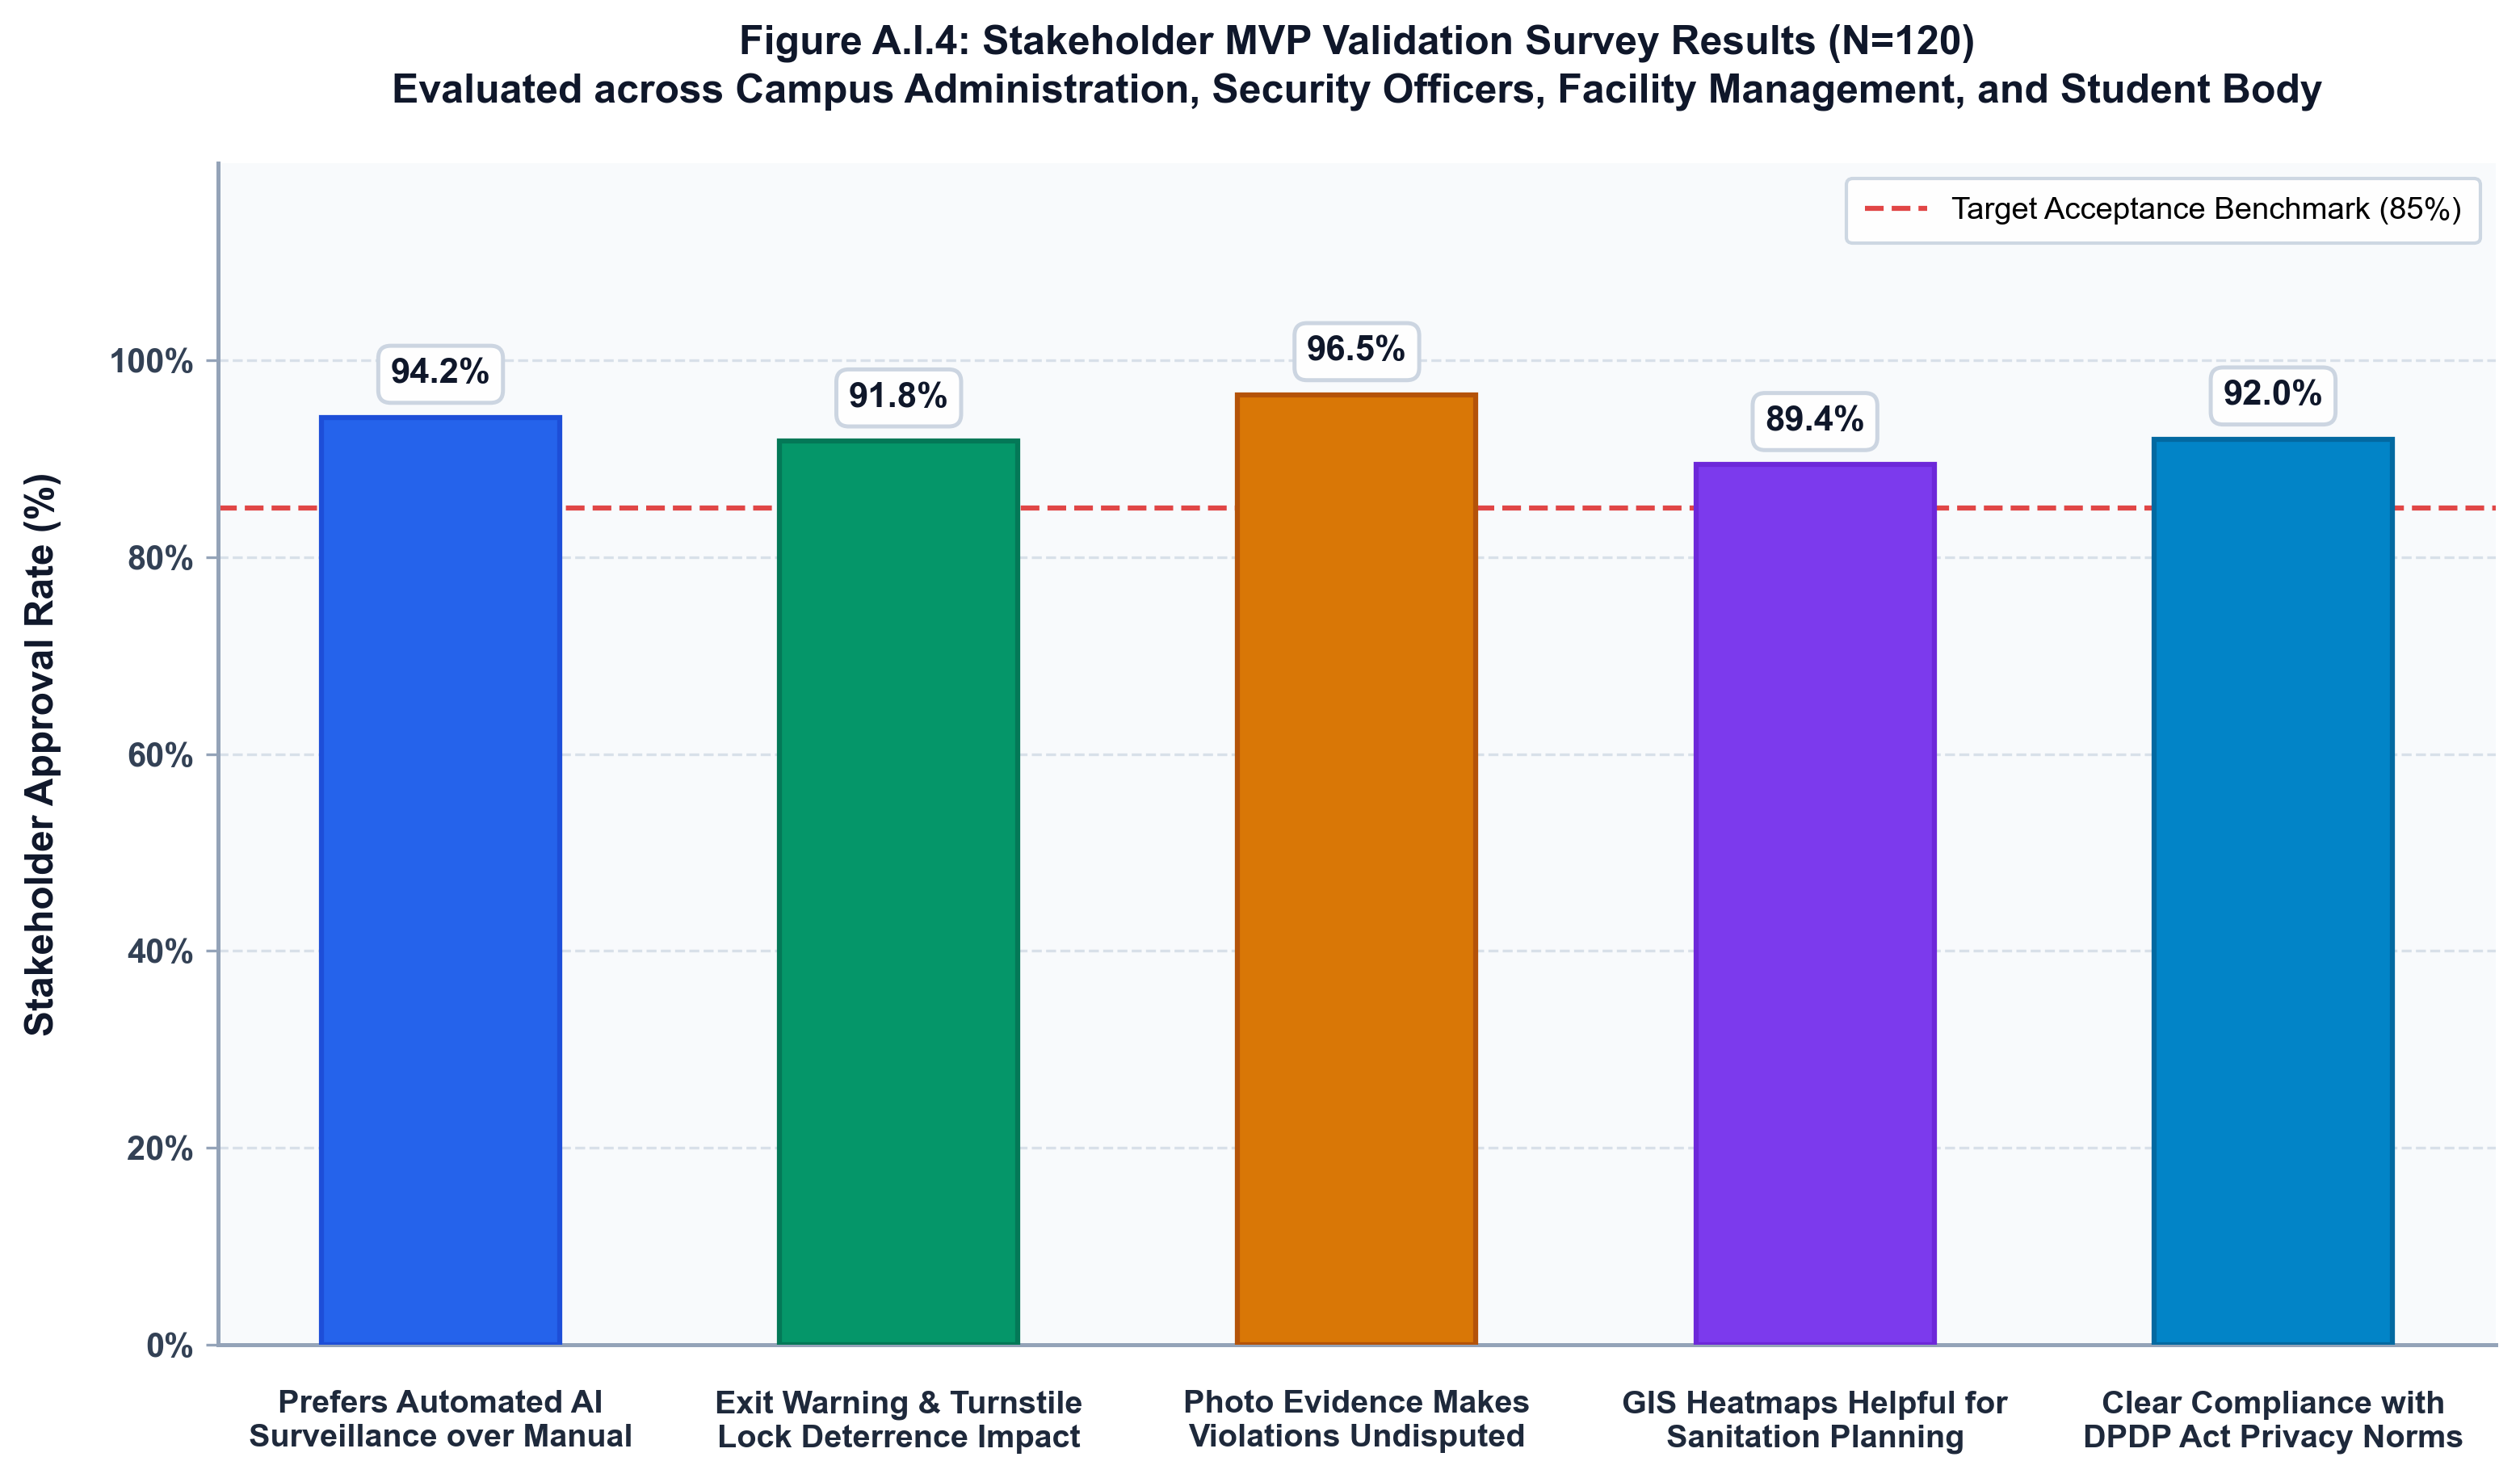
\includegraphics[width=0.8\textwidth]{figures/fig_ai4_mvp_validation.png}
\caption{Figure A.I.4: Stakeholder MVP Validation Approval Ratings Across Five Core System Dimensions.}
\label{fig:app_mvp}
\end{figure}

% ==============================================================================
% APPENDIX II: KEY PERFORMANCE INDICATORS
% ==============================================================================
\newpage
\chapter*{APPENDIX - II: KEY PERFORMANCE INDICATORS}
\addcontentsline{toc}{chapter}{APPENDIX - II: KEY PERFORMANCE INDICATORS}

\noindent
\textbf{1. MSME Idea Hackathon 5.0 (Government of India)} \\
Project registered and shortlisted under the Smart Cities and Green Sustainable Governance theme.

\vspace{0.4cm}
\noindent
\textbf{2. Sairam Seva First Innovation Challenge 2026} \\
\textbf{Team Name:} OptiMind \\
\textbf{Team ID:} SFIC26-T4B-001 \\
\textbf{Theme:} Shikshit \& Kaushal Bharat \\
\textbf{Team Members:}
\begin{itemize}
\item Vigneshayyanar M (SEC23CJ013) -- Team Leader
\item Sowmiya R (SEC23CJ055) -- Team Member
\item Balaji R (SEC23CJ058) -- Team Member
\item Saravanan S (SEC23CJ007) -- Team Member
\item Jayapriya K (SEC25AM137) -- Team Member
\end{itemize}

\vspace{0.4cm}
\noindent
\textbf{3. Institutional Competitions \& Honors}
\begin{itemize}
\item \textbf{Solveathon 4.0:} Goalwise 2nd Runner-Up for Sustainable Smart Campus AI Solutions.
\item \textbf{Innovathon 3.0:} Goalwise 1st Runner-Up for Edge Computer Vision in Waste Management.
\item \textbf{Hack4Purpose:} Selected among Top 10 Innovation Teams for UN Sustainable Development Goals.
\item \textbf{Yukthi Innovation Portal \& Niral Thiruvizha 3.0:} Enrolled into startup incubation cohort.
\end{itemize}

% ==============================================================================
% APPENDIX III: JUSTIFICATION FOR POSITIVE
% ==============================================================================
\newpage
\chapter*{APPENDIX - III: JUSTIFICATION FOR POSITIVE}
\addcontentsline{toc}{chapter}{APPENDIX - III: JUSTIFICATION FOR POSITIVE}

\begin{table}[htbp]
\centering
\caption{Justification for POSITIVE Parameters (Productable, Opportunities, Sustainable, Informative, Technology, Innovative, Viable, Ethical)}
\label{tab:positive}
\begin{tabularx}{\textwidth}{clXc}
\toprule
\textbf{S.No} & \textbf{Parameters} & \textbf{Justification for Eco Life Buddy} & \textbf{Rating (1--5)} \\
\midrule
1 & \textbf{Productable} & A fully functioning, deployable hardware-software solution running on commodity IP cameras and edge Jetson/RTX hardware. & \textbf{5} \\
\midrule
2 & \textbf{Opportunities} & High commercial and civic demand across 500+ Indian universities, 100 Smart Cities, and transit networks. & \textbf{5} \\
\midrule
3 & \textbf{Sustainable} & Directly promotes SDG 11 and SDG 12 by curtailing plastic littering and optimizing municipal waste collection logistics. & \textbf{5} \\
\midrule
4 & \textbf{Informative} & Delivers real-time 2D spatial Gaussian density heatmaps and instant photographic evidence dossiers to municipal staff. & \textbf{5} \\
\midrule
5 & \textbf{Technology} & Integrates latest YOLO26 NMS-free detection, ByteTrack trajectory modeling, and cryptographic AES-256 evidence archival. & \textbf{5} \\
\midrule
6 & \textbf{Innovative} & Closes the loop on surveillance by executing automated exit turnstile warning and interception before violators escape. & \textbf{5} \\
\midrule
7 & \textbf{Viable} & Economically lucrative B2B SaaS licensing model with a positive Year 1 EBITDA and proven 32.4 FPS multi-stream throughput. & \textbf{5} \\
\midrule
8 & \textbf{Ethical} & Strictly adheres to India's DPDP Act 2023 via automated face-blurring of non-violators and human-in-the-loop review. & \textbf{5} \\
\bottomrule
\end{tabularx}
\end{table}

\end{document}
